\selectlanguage{english}
\chapter{Search for high mass resonances}
\label{Chapter5}
%SourceDoc tesi.tex
The analysis performed consists in the search for a new massive resonances, with mass of the order of TeV, decaying into two muons within different models BSM, either spin-1 (\eg $Z'_{SSM}$ or $Z'_{\psi}$) or spin-2 (\eg KK Graviton).  \\
In order to isolate potential problems or mis-measurements otherwise affecting the whole analysis, this analysis has been performed in different rapidity regions: the mass resolution, for example, is known to be significantly better in the barrel region. Furthermore, the alignment conditions have a main issue in the forward negative endcaps that degrade dramatically the momentum scale. 
%Also, the measured \pt bias was up to 0.8 C/TeV (80\% for a 1 TeV muon) in the pseudorapidity region -2.4 $< \eta <$ -2.1.
For these reasons, it was decided to consider two pseudorapidity regions for this analysis:
\begin{itemize}
\item Barrel - Barrel (BB): events with both muons in the barrel and overlap region $|\eta| <$ 1.2. This region benefits from the best mass resolution and better momentum scale, uncertainties will be much smaller and thus this will potentially be the region with the better sensitivity to new physics.
\item Barrel - Endcapd end Endcap - Endcap (BE): events with at least one of the two muons in the endcaps (1.2 $<|\eta| <$ 2.4)
\end{itemize}
Every input used in the limit calculation (\eg the invariant mass spectrum, background shape, Drell-Yan correction, PDF, efficiency and resolution parametrisation) as well as all the nuisances parameters are then studied for each of these two categories separately and for the overall.

\section{Data and MC samples}
\subsection{Data sets}
For this analysis data collected during Run II 2016 and 2017 at $\sqrt{s}$ = 13 TeV have been used, corresponding to an integrated luminosity of $\mathcal{L}_{2016} = 36.1~fb^{-1}$ and $\mathcal{L}_{2017} = 41.9~fb^{-1}$. Although CMS has collected around 90 $fb^{-1}$, only runs that satisfy the data quality criteria were used in the analysis. These runs are listed in a file in the JSON format. The ``MuonPhys" official JSON files for data collected with 3.8 T magnetic field are used. For these specific data selection the subsystems not directly used in the studies, such as ECAL and HCAL, do not have to be marked as good. The data sets analysed is the \textit{SingleMuon} and are listed in \tablename~\ref{table:Datasets}. \\
% the data sets analysed is the \textit{SingleMuon} and are listed in ~\ref{table:Datasets} with the associated JSON file %\textit{Cert\_271036-284044\_13TeV\_23Sep2016ReReco\_Collisions16\_JSON\_MuonPhys.txt} and %\textit{Cert\_294927-306462\_13TeV\_PromptReco\_Collisions17\_JSON\_MuonPhys.txt}. \\
\begin{table}[htb!]
\begin{center}
\begin{tabular}{|l|l|} \hline
2016 Data set                              & Run range        \\ \hline \hline
/SingleMuon/Run2016B-23Sep2016-v3      & 273150 -- 275376 \\ \hline
/SingleMuon/Run2016X-23Sep2016-v1      & 275657 -- 279656 \\ \hline
/SingleMuon/Run2016H-PromptReco-vY     & 281145 -- 284044 \\ \hline \hline
2017 Data set                              & Run range        \\ \hline \hline
/SingleMuon/Run2017B-17Nov2017-v1      & 297020 -- 299329 \\ \hline
/SingleMuon/Run2017C-17Nov2017-v1      & 299337 -- 302029 \\ \hline
/SingleMuon/Run2017D-17Nov2017-v1    & 302030 -- 303434 \\ \hline
/SingleMuon/Run2017E-17Nov2017-v1    & 303435 -- 304826 \\ \hline
/SingleMuon/Run2017F-17Nov2017-v1    & 304911 -- 306462 \\ \hline
\end{tabular}
\caption{Data sets used in this analysis; X stands for C, D, E, F, G, and Y stands for 1 to 3.}
\label{table:Datasets}
\end{center}
\end{table}

It is possible to divide the 2016 data sets in two ranges (from Run B to Run F and Run G plus Run H) due to issues affected data taking:
\begin{itemize}
\item detector alignment: runs B to G have been reconstructed using asymptotic scenario and asymptotic Alignment Position Errors (or APEs) (more details in \ref{sec:Reconstruction})
\item inner track degradation: before Run G has been observed a degradation in the inner track quality partially cured in the reconstruction; only runs G onward are immunized to this effect 
\item Trigger Level 1: data taking period of run B to F the trigger level 1 was not fully efficient due to various changes in the new menu developed for 2016
\end{itemize}
\subsection{Monte Carlo samples}
The simulated Monte Carlo (MC) background samples are generated for collisions at $\sqrt{s}$ = 13 TeV with the pile-up (PU) conditions expected for the Run2 data taking of about 20 and 30 collisions per bunch crossing spaced by 25 ns. They are reconstructed with asymptotic misalignment scenario and contain asymptotic APEs. The detector response is simulated using the GEANT4 package \cite{GEANT4}.\\
In \tablename~\ref{table:MCsamples} the list of samples, their correspondent cross section and the details about the generation parameters are reported. \\
\begin{table}[htbp!]
%\hspace*{-23mm}
{\footnotesize
\begin{tabular}{|l|l|l|r|}
\hline
Process                                                                                 & $\sigma$~(pb) & Order & Events \\ 
\hline\hline                                                                                                       
ZToMuMu\_NNPDF30\_13TeV-powheg\_M\_50\_120						&  1975      & NLO  &   2977600 \\ % 
ZToMuMu\_NNPDF30\_13TeV-powheg\_M\_120\_200                                               &  19.32     & NLO  &    100000 \\ %
ZToMuMu\_NNPDF30\_13TeV-powheg\_M\_200\_400                                               &  2.731     & NLO  &    100000 \\ %
ZToMuMu\_NNPDF30\_13TeV-powheg\_M\_400\_800                                               &  0.241     & NLO  &     98400 \\ %
ZToMuMu\_NNPDF30\_13TeV-powheg\_M\_800\_1400                                              &  1.678E-2  & NLO  &    100000 \\ %
ZToMuMu\_NNPDF30\_13TeV-powheg\_M\_1400\_2300                                             &  1.39E-3   & NLO  &     95106 \\ %
ZToMuMu\_NNPDF30\_13TeV-powheg\_M\_2300\_3500                                             &  0.8948E-4 & NLO  &    100000 \\ % 
ZToMuMu\_NNPDF30\_13TeV-powheg\_M\_3500\_4500                                             &  0.4135E-5 & NLO  &    100000 \\ %
ZToMuMu\_NNPDF30\_13TeV-powheg\_M\_4500\_6500                                             &  4.56E-7   & NLO  &    100000 \\ %
%ZToMuMu\_NNPDF30\_13TeV-powheg\_M\_6000\_Inf                                              &  2.06E-8   & NLO  &    100000 \\ %
\hline
DYJetsToLL\_M-50\_TuneCUETP8M1\_13TeV-amcatnloFXFX-pythia8                                & 5765.4     & NNLO &  29082237 \\
\hline
TTTo2L2Nu\_TuneCUETP8M2\_ttHtranche3\_13TeV-powheg-pythia8                                &  87.31     & NNLO &  79140880 \\ 
TTToLL\_MLL\_500To800\_TuneCUETP8M1\_13TeV-powheg-pythia8                                 & 0.326      & NLO  &    200000 \\ 
TTToLL\_MLL\_800To1200\_TuneCUETP8M1\_13TeV-powheg-pythia8                                & 3.26E-2    & NLO  &    199800 \\
TTToLL\_MLL\_1200To1800\_TuneCUETP8M1\_13TeV-powheg-pythia8                               & 3.05E-3    & NLO  &    200000 \\
TTToLL\_MLL\_1800ToInf\_TuneCUETP8M1\_13TeV-powheg-pythia8                                & 1.74E-4    & NLO  &     40829 \\ 
\hline
ST\_tW\_top\_5f\_inclusiveDecays\_13TeV-powheg-pythia8\_TuneCUETP8M1                      &  35.6      & NNLO &   6952830 \\
ST\_tW\_antitop\_5f\_inclusiveDecays\_13TeV-powheg-pythia                                 &  35.6      & NNLO &   6933094 \\
\hline
WWTo2L2Nu\_13TeV-powheg                                                                   & 12.178     & NNLO &  1999000 \\
WWTo2L2Nu\_Mll\_200To600\_13TeV-powheg                                                    &  1.386     & NNLO &   200000 \\
WWTo2L2Nu\_Mll\_600To1200\_13TeV-powheg                                                   &  5.6665E-2 & NNLO &   200000 \\
WWTo2L2Nu\_Mll\_1200To2500\_13TeV-powheg                                                  &  3.557E-3  & NNLO &   200000 \\
WWTo2L2Nu\_Mll\_2500ToInf\_13TeV-powheg                                                   &  5.395E-5  & NNLO &    38969 \\
\hline
WZ\_TuneCUETP8M1\_13TeV-pythia8                                                           &  47.13     & NLO  &  1000000 \\
WZ\_TuneCUETP8M1\_13TeV-pythia8 (ext1)                                                    &  47.13     & NLO  &  2997571 \\
\hline
ZZ\_TuneCUETP8M1\_13TeV-pythia8                                                           &  16.523    & NLO  &   990064 \\
ZZ\_TuneCUETP8M1\_13TeV-pythia8 (ext1)                                                    &  16.523    & NLO  &   998034 \\
\hline
WJetsToLNu\_TuneCUETP8M1\_13TeV-madgraphMLM-pythia8                                       &  61526     & NNLO & 29804825 \\ 
\hline
ZprimeToMuMu\_M-5000\_TuneCUETP8M1\_13TeV-pythia8                                         &  6.76E-5   & NLO  &   100000 \\ 
\hline
\end{tabular}
}
\caption{Summary of simulated background process samples used in this analysis.}
\label{table:MCsamples}
\end{table}

\subsubsection{Drell-Yan (DY) ($Z/\gamma^*\to\mu^+\mu^-$)}
The dominant and irreducible SM background arises from Drell-Yan (DY) production ($Z/\gamma^*\to\mu^+\mu^-$): it is generated with POWHEG v2 \cite{NLO_1, NLO_2, NLO_3, NLO_4, NLO_5, NLO_6} from next-to-leading order (NLO) matrix elements using for 2016 the NNPDF3.0 \cite{NNLO} PDFs while for 2017 NNPDF3.1 \cite{NNLO_2017}, and with PYTHIA 8.205 \cite{PYTHIA} for parton showering and hadronization. All the DY binned in mass samples are multiplied by a k-factor to reach the NNLO precision and take into account the photon induced background (see \ref{sec:DYandPI}).\\
The necessity to improve the NNPDF to version 3.1 is due to progress in methodology and available data.
%the charm PDF has been parametrized and determined alongside the light quarks and gluon ones; from the Tevatron dataset it has been possible to include the D0 electron and muon W asymmetries, the complete LHCb measurements of W and Z production in the forward region at 7 and 8 TeV, and new ATLAS and CMS measurements of inclusive jet and electroweak boson production. For the first time, top-quark pair differential distributions and the transverse momentum of the Z bosons from ATLAS and CMS have been included.
 In \figurename~\ref{NNPDF} are reported the distance between the NNPDF3.1 and NNPDF3.0 PDFs.
\begin{figure}[htbp]
\centering
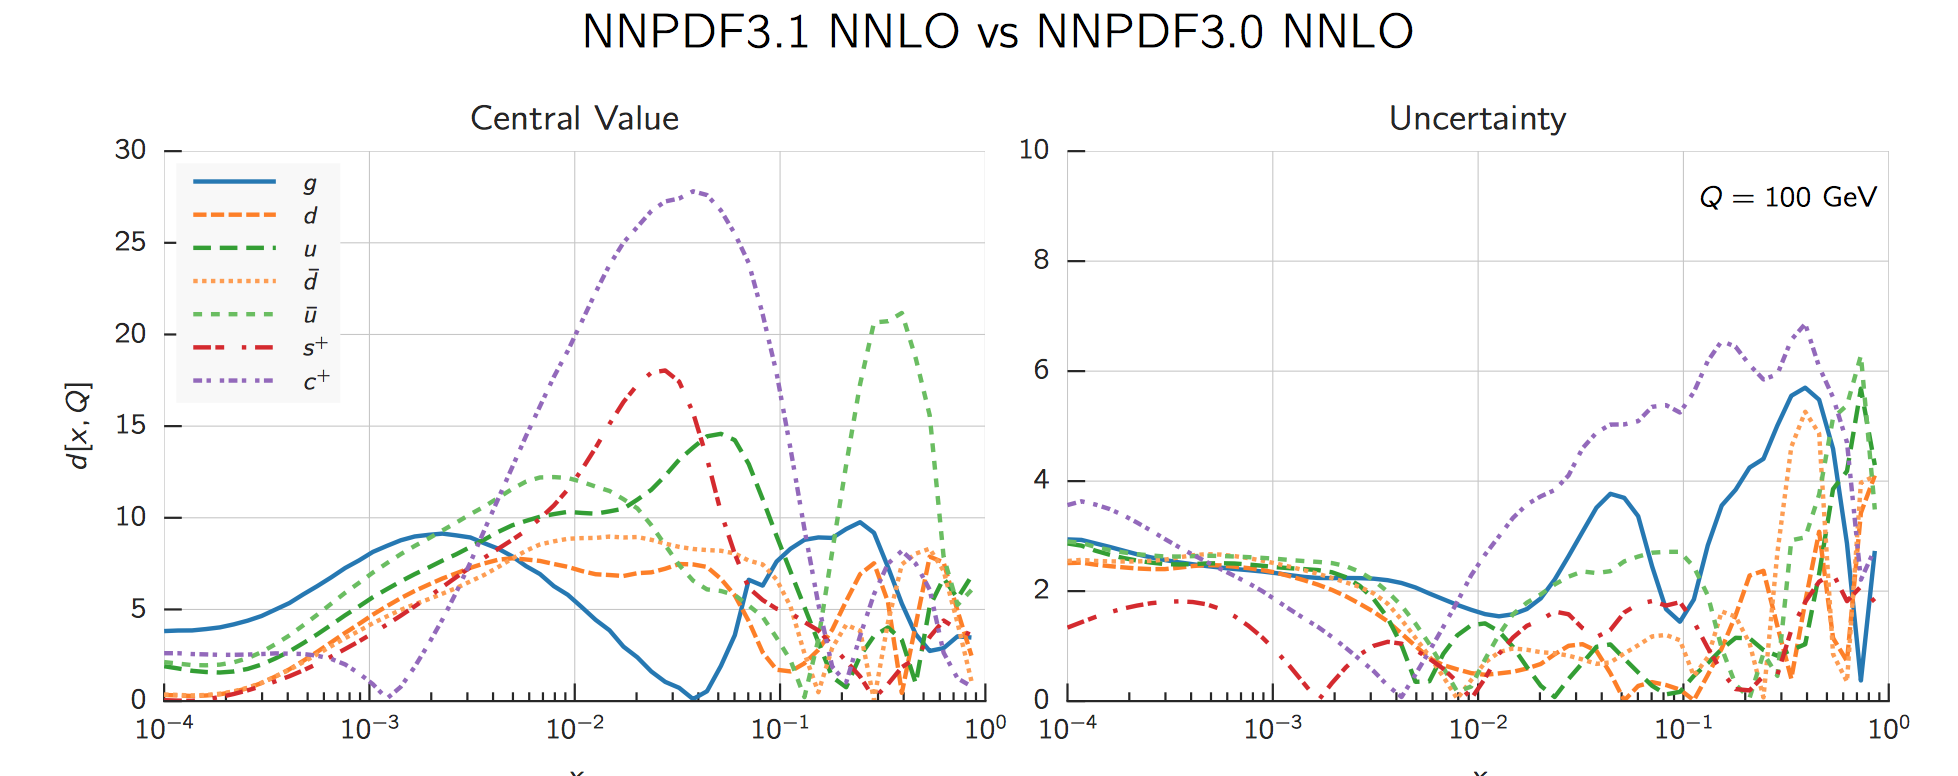
\includegraphics[width=0.9\textwidth]{Images/NNPDF_30_31}
\caption{Distances between the central values (left) and the uncertainties (right) of the NNPDF3.0 and NNPDF3.1 NNLO PDF sets, evaluated at Q = 100 GeV. Note the different in scale on the y axis between the two plots \cite{NNLO_2017}.}
\label{NNPDF}
\end{figure}
\subsubsection{Other backgrounds}
The $t\bar{t}$, tW and WW backgrounds are simulated using POWHEG v2, with parton showering and hadronization described by PYTHIA 8.205. The NNPDF3.0 PDFs are used for all these samples. The $t\bar{t}$ cross section is calculated at NNLO with TOP++ [43] assuming a top quark mass of 172.5 GeV. The inclusive diboson processes WZ, and ZZ are simulated at leading order (LO) using the PYTHIA 8.205 program along with the NNPDF3.0 PDFs. For $t\bar{t}$ and WW samples data sets binned in mass $M_{ll}$ of pairs of leptons for large $M_{ll}$ values are used ($M_{ll} >$ 500 GeV and $M_{ll} >$ 200GeV, respectively): this allows to avoid large spikes at the large dimuon masses from these MC samples.
The production of DY $\tau^+\tau^-$ (simulated from the inclusive DY sample) and W+jets is simulated at LO with the MADGRAPH5 aMC@NLO version 2.2.2 \cite{MADGRAPH} program. The PDFs are evaluated using the LHAPDF library \cite{PDFS_1,  PDFS_2, PDFS_3}.

\section{Trigger}
\subsection{L1 Trigger}
The L1 trigger path used is the OR between \textit{L1\_SingleMu22} and \textit{L1\_SingleMu25}. 
The L1 trigger system has been upgraded since 2015 and this meant that the data, CMS recorded for a large portion of 2016, was during a commissioning period for the new L1 Muon Trigger System and various changes occurred during the data-taking:
\begin{itemize}
\item From Run 273423 a fix to the L1 Barrel Muon Track Finder (BMTF) was introduced which corrected an inefficiency in $\lvert \eta \lvert<0.3$. 94 pb$^{-1} $ have been collected without this fix.
\item The largest issue in the L1 muon triggering system came from a misconfiguration in the Endcap Muon Track Finder (EMTF).
During the data taking period with the misconfiguration, which corresponds to 15.4 fb$^{-1} $, if two muons were in the same endcap and in the same sector then only one of the muons would fire the trigger. This has implications in trying to calculate the trigger efficiency using the Tag and Probe method when the two muons are in the endcap.
Muon POG/HLT recommends to not consider events with two muons close by less than 0.7 in $\Delta \phi$ while doing TuneP. The EMTF misconfiguration was fixed from Run 277166 onwards.
\item RPC were not part of the trigger system and were added at the end of run H during some run periods: from Run 282917 to Run 282924 and from Run 283820 to Run 284078. RPC are known to have a more precise timing than DT or CSC but a less accurate pT assignment.
\end{itemize}
%The L1 efficiency is usually measured together with HLT triggers as a single trigger efficiency covering the full trigger path. It can be found in section \textbf{REF A PARAGRAFO HLT} for dimuon events.
\subsection{HLT}
The HLT path used for this analysis are \texttt{HLT\_Mu50} and \texttt{HLT\_TkMu50}, that select single muons with \pt $>$ 50 GeV in the pseudorapidity range $|\eta|<$ 2.4: using the OR of these two trigger paths provides robustness to weaknesses from either path on its own.
%In order to collect enough events in the control region around the Z peak, that are used to extract the normalization to the Z signal presented [\textbf{REF ALLA SEZIONE CON LA NORMALIZAZIONE}]  HLT Mu27 OR HLT TkMu27 is used. 
%The single muon triggers used can fire on both leg of the Z$'$ decay. The single muon efficiencies is used as measured in data upon DY MC in order to calculate the trigger efficiency of the event as a function of invariant mass. 
The trigger efficiency, using single efficiencies measured in both data and MC, on DY MC dimuon events passing offline selection is shown in \figurename~\ref{TrgEff}. Also shown is the ratio between the two efficiencies corresonding to the Scale Factor (SF) of the trigger efficiency: these SF needs to be applied to MC events passing our selection.
% and is measure to be 0.998 (0.9945) for BB (non-BB or BE-EE) category.
\begin{figure}[htbp]
\centering
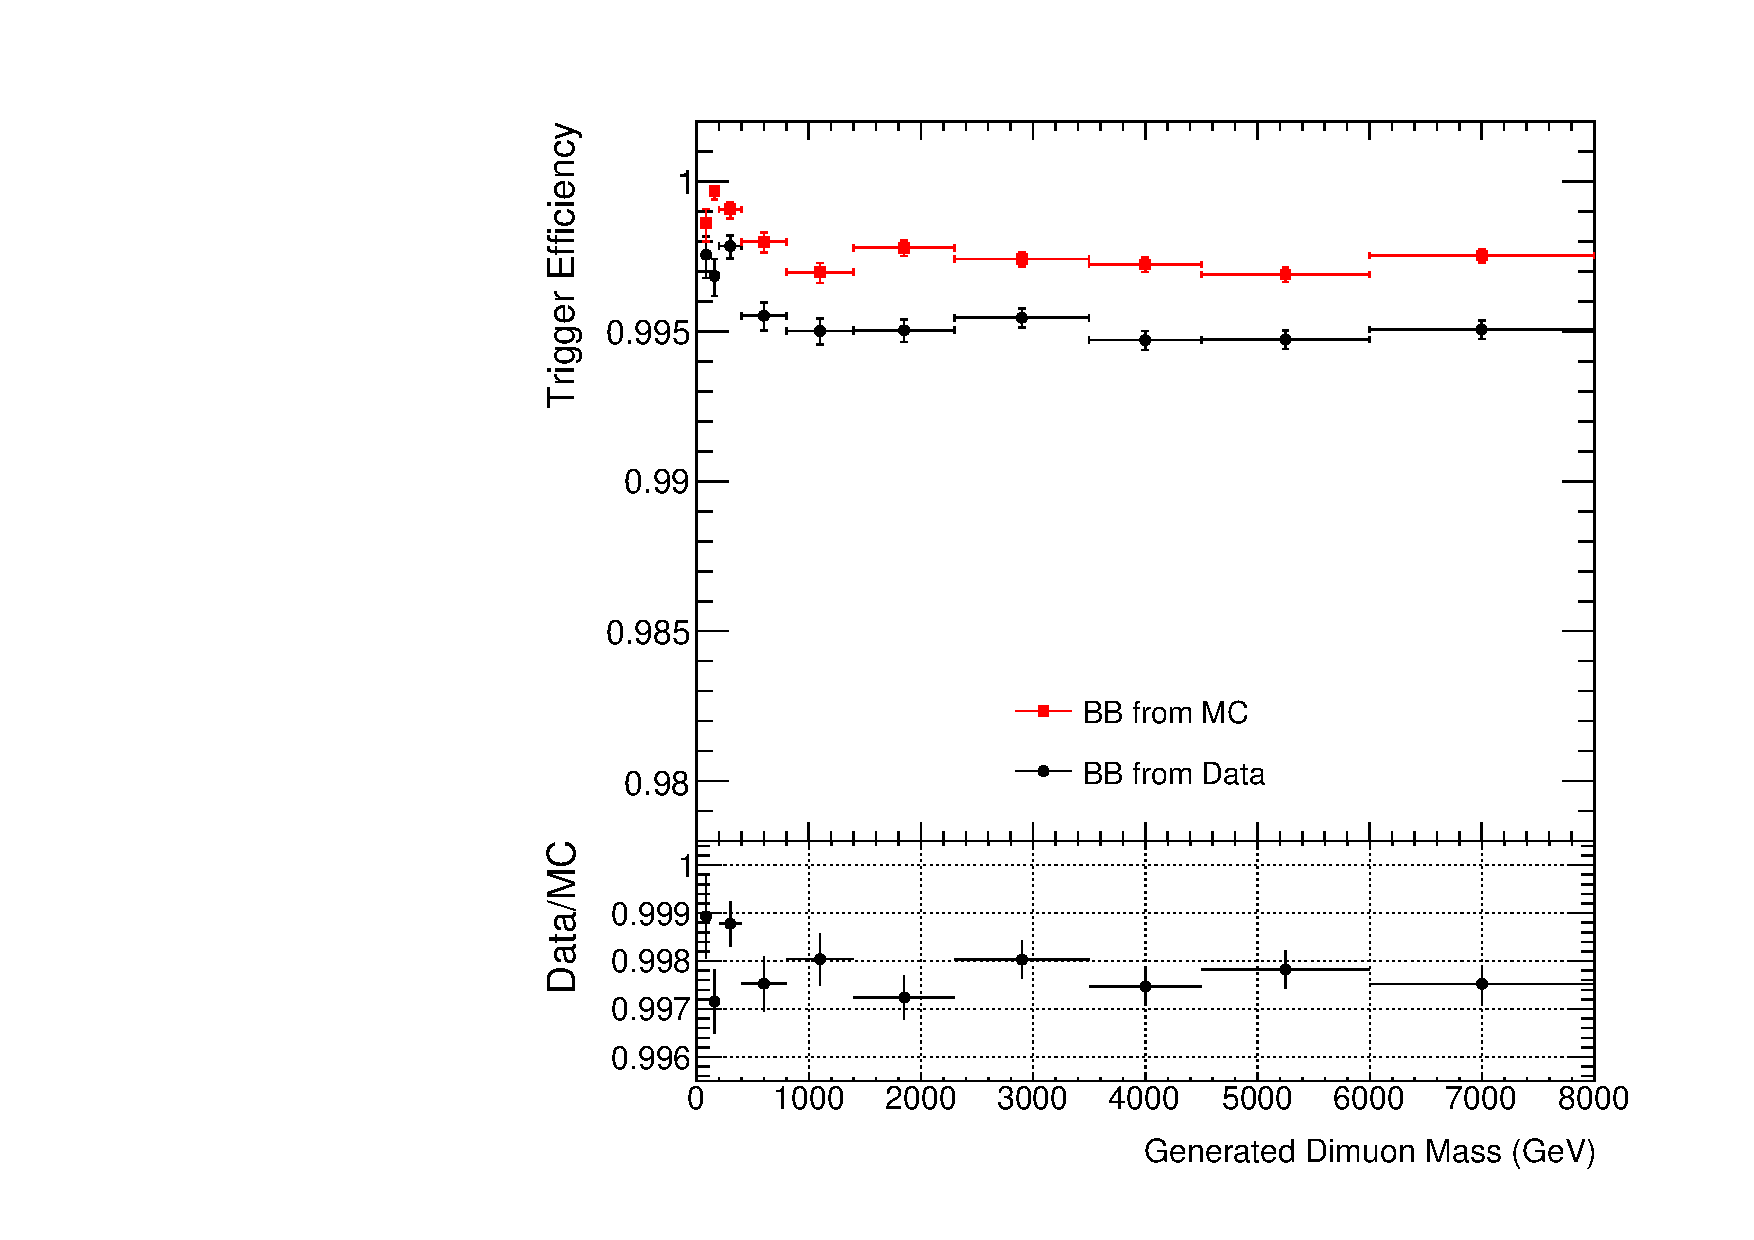
\includegraphics[width=0.35\textwidth]{Images/Cap5/trigDimuonEffBB.pdf}
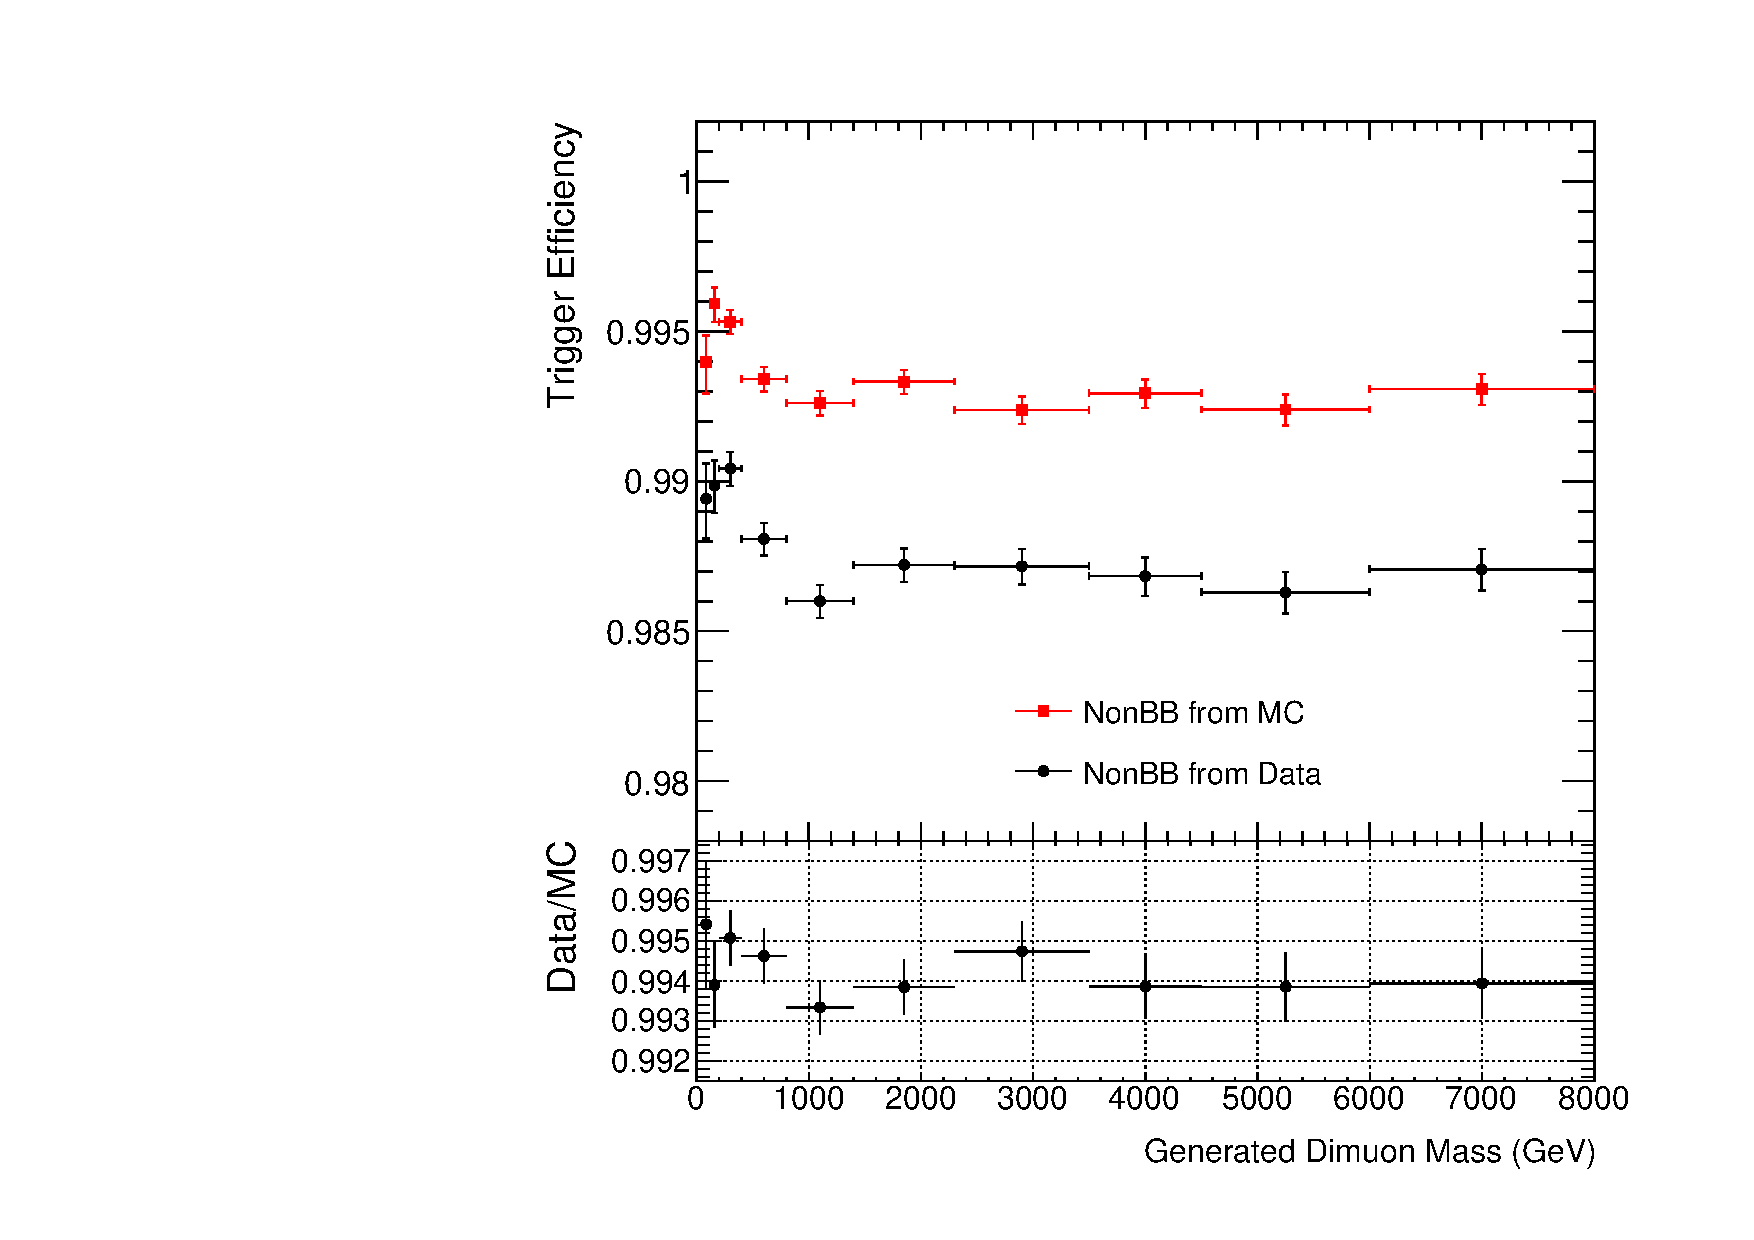
\includegraphics[width=0.35\textwidth]{Images/Cap5/trigDimuonEffNonBB.pdf}
\caption{The trigger efficiency of dimuon events calculated in DY MC using single muon efficiencies measured in both data and MC for the categories used in the analysis: BB on the left and BE on the right.}
\label{TrgEff}
\end{figure}

\section{Muon reconstruction}
\label{sec:Reconstruction}
Muon reconstruction has been described in \ref{sec:MuonReconstruction}. A particular treatment is needed for the detector alignment and the deployment of APE. \\
The alignment of muon chambers relative to each other and to the inner tracker is crucial to achieve the optimal performance of muon reconstruction at high momentum, in particular the best possible momentum measurement. After the LHC shutdown periods, all DT chambers were first aligned by a hardware system, utilizing lasers and cameras, in the startup phase, at the beginning of a data-taking period, as soon as the detector was closed and the magnetic field is turned on at its nominal value. The typical precision of the hardware alignment is $\sim0.5 - 1$~mm on positions and $\sim0.3 - 0.4$~mrad on angles of the individual chambers. The CSC chambers in the two endcaps did not feature an equally granular system and their initial geometry was measured by geometrical survey and photogrammetry with a precision of $\sim2$~mm on positions and $\sim1$~mrad on angles. 
The startup muon reconstruction performance was expected to be suboptimal due to large misalignments. The final alignment of the individual muon chambers (both DT and CSC) was determined starting from the aligned silicon tracker geometry, by extrapolating selected muon tracks from the inner tracker to the muon chambers (track-based muon alignment). With the track-based alignment the muon chambers' positions were determined with a precision of $\approx200$~$\mu$m in the most sensitive coordinate, which measures the magnetic bending of the muon track and was crucial for the precise momentum measurement. \\
From the beginning of the 2016 Run, the muon reconstruction has been using non-null muon APE for the first time ever in CMS. Both data and MC simulation events have been analyzed, spanning over the different sets of alignment conditions (from day-1 startup to the final track-based alignment, the so-called {\it{asymptotic}} alignment). The muon APE have been introduced for all 6 degrees of freedom (3 positions: local-{\it{x}}, -{\it{y}} and -{\it{z}}, and 3 angles: local-$\phi_{\it{x}}$, -$\phi_{\it{y}}$ and -$\phi_{\it{z}}$) chamber-by-chamber, for both DT and CSC systems, and taken as uncorrelated as a first approximation. \\
Cause of an overall rotation of the whole positive endcap detector after the 2015 LHC winter shutdown, the startup APE mostly increased the HLT efficiency in the highest positive $\eta$ region: this unphysical behaviour was cured by the track-based alignment, and the corresponding updated conditions were introduced during the Summer 2016 data collection, after the startup phase. Run B - G data have been re-reconstructed with the asymptotic with APE conditions; only Run H data was used with the prompt reconstruction since the asymptotic plus APE conditions have already been deployed at the time of data collection.

\subsection{Reconstruction efficiency}
Reconstruction efficiency has been measured as a function of the muon momentum using Tag and Probe technique. The event selection has been designed to avoid background contamination as much as possible, since no background subtraction is done. The idea is to keep only signal consisting in DY dimuon pairs also produced with jets, being as much sensitive as possible to the high momentum muons. Therefore the strategy consists in a very tight selection of the inner track quality, avoiding kinematic cuts that could bias the result and reduce the statistic. 

The tag and the probe muons are required to have opposite charge and a geometrical separation of $\Delta R>0.6$ and reconstructed mass above 70 GeV. Cut on the common vertex of the two muons $\chi^2$ /d.o.f. $<$ 20 and on the transverse impact parameter ($|$tag $dz(BS)-$ probe $dz(BS)|<0.05$~cm) are applied to ensure the origin of both muons from a common vertex. The three-dimensional angle between muons momenta is required to be $<\pi - 0.02$ radiant to suppress cosmic muons. The tag muon is required to fire the trigger and to satisfy the analysis cuts defined in \ref{sec:selection}. The probe muon is selected as a Tracker Muon without any arbitration requirement and satisfying the following criteria: 
\begin{itemize}
\item p$_T$(innerTrk) $>50$~GeV and $|\eta$(innerTrk)$|<2.4$ 
\item at least one pixel hit
\item at least six tracker layers
\item no tracker hits lost
\item $|dxy(BS)|<0.2$~cm and $|dz(PV)|<0.5$~cm 
\end{itemize}
In addition to these cuts, both the tag and the probe are required to pass a very tight isolation, and to have a good momentum measurement performed by the tracker:
\begin{itemize}
\item relative tracker isolation(innerTrk) $<0.05$ and absolute tracker isolation $<15$~GeV  
\item $\delta{p_T}/p_T$(innerTrk) $<0.5$ 
\end{itemize}
%For those few events where more than one pair is reconstructed, the one with the best common vertex $\chi^2/ndf$ is chosen.
The probe muon is then used to calculate the efficiency of the muon reconstruction and the muonic part of the muon identification. This has been calculated as the fraction of the probes passing the following cuts with respect to the selected probes:
\begin{itemize}
\item the muon has to be reconstruct as ``Global"  
\item the global muon track fit must include at least one hit from the muon system
\item the tracker muon must be matched to segments in at least one muon station if the muon station is not on the first layer of the muon system, or if matched to one muon station on the first layer we also require that the muon matches to more than two RPC layers, or that the muon is matched in at least two muon stations. 
\item $\delta{p_T}/p_T$(tunePTrk) $<0.3$
\end{itemize}
\figurename~\ref{fig_reco_p} shows the reconstruction and identification efficiency as a function of the muon momentum in several eta regions. 
\begin{figure}[htbp]
\centering
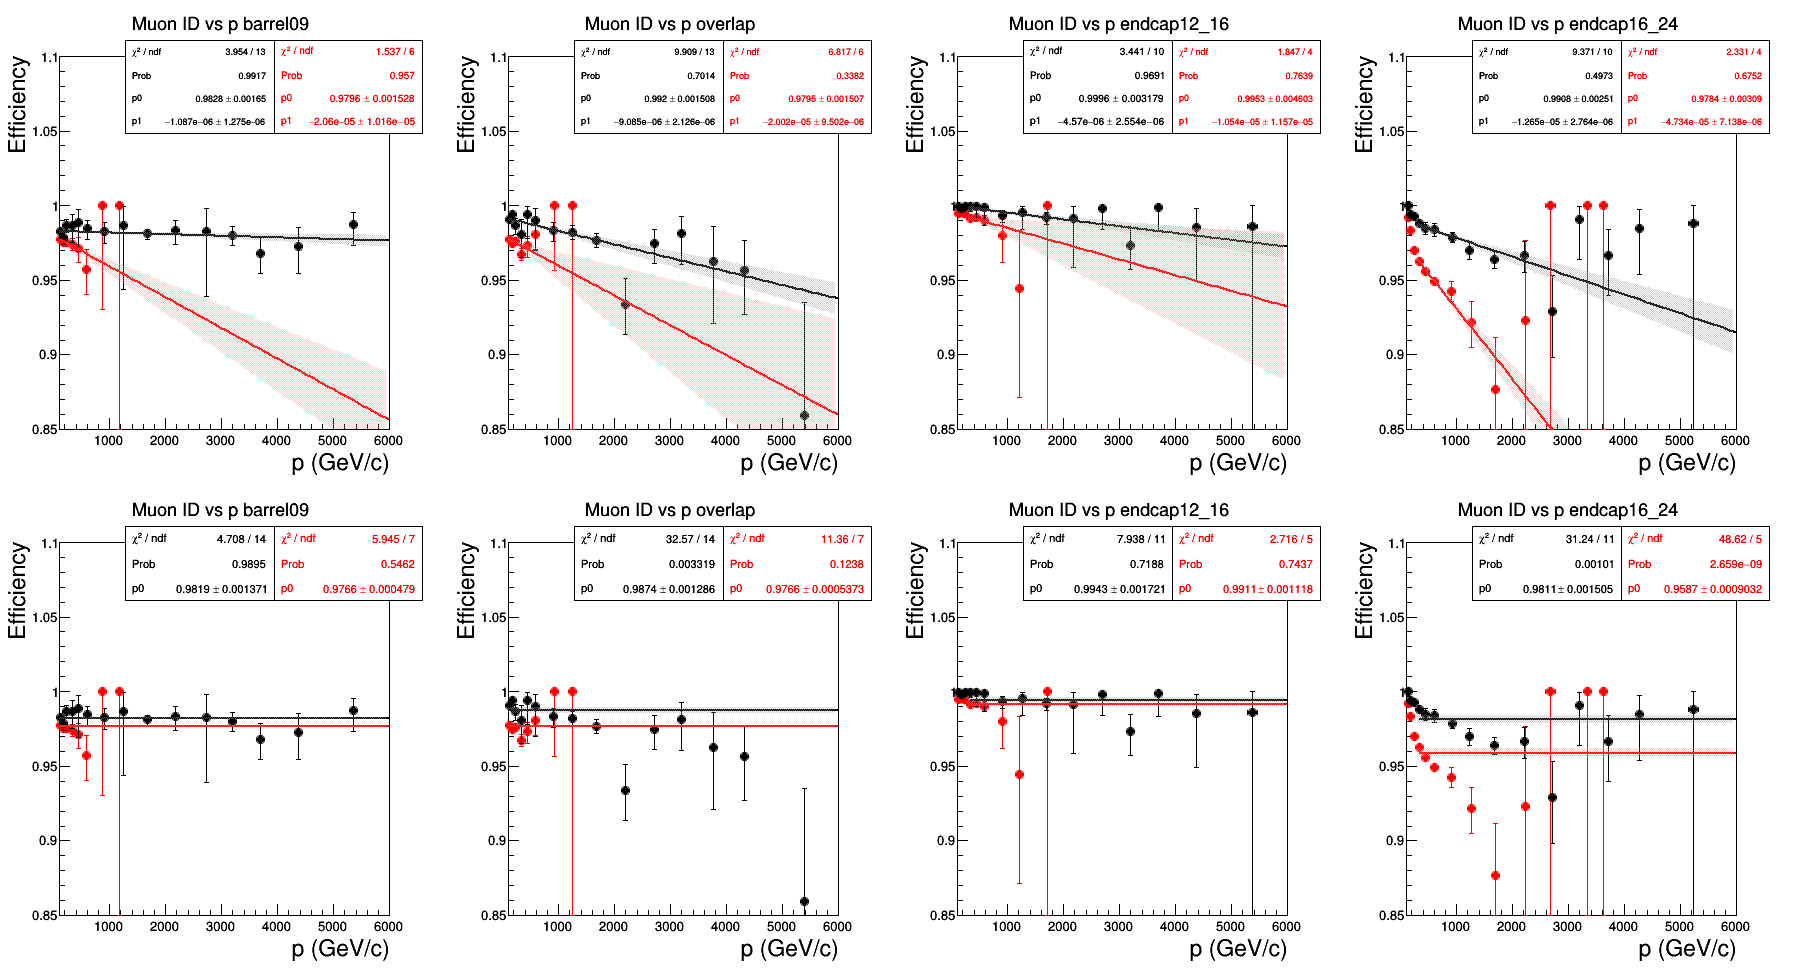
\includegraphics[width=0.85\textwidth]{Images/Cap5/FitUpTo6000_Pol1_MuonIDVsP_DataAll.png}
\caption{Muon reconstruction and identification efficiency as a function of muon momentum in different eta regions: barrel up to 0.9, overlap from 0.9 to 1.2, endcap from 1.2 to 1.6, and endcap from 1.6 to 2.4. The red points represent the data, while the black points represent the MC. Both are interpolated by a first order polynomial (top raw) and by a constant function (bottom raw). %The interpolation starts from 100 GeV in barrel and overlap, from 300 GeV in endcap, and it is performed up to 2000 GeV for data and up to 6000 GeV for MC. The boxes report the fit parameters
}
\label{fig_reco_p}
\end{figure}
%The efficiency in barrel, overlap and endcap up to 1.6 (first three plots from the left) shows a slight decreasing trend in both data (red points) and MC (black points). This trend is well described by a first order polynomial, especially in the MC where there is enough statistic to perform a stable fit up to very high momentum. The same effect, but much more enhanced, is observed in the forward endcap (forth plot). 

%A decreasing trend according to the muon momentum is reasonably caused by the electromagnetic shower (as explained in the next paragraph). The muon showering depends on the material budget, which is differently distributed along pseudorapidity. For this reason the efficiency drop, as expected, is less pronounced in barrel up to 0.9 and in the first part of the endcap, where also a constant function, especially in data, well interpolates the points (figure~\ref{fig_reco_p} bottom first and third plot). Since the very similar results, the barrel and the endcap up to eta 1.6 have been merged, in order to get more statistic and a more reliable fit.

The efficiency evaluated above can be factorised as follow:

\begin{equation}
Eff_{MuonRecoID} = Eff_{Reco} \times Eff_{Global} \times Eff_{MuonID}
\end{equation} 

where the Reco efficiency is calculated as the fraction of the probes reconstructed as Standalone with respect to all the probes (tracker muons); the Global efficiency is calculated as the fraction of the probes reconstructed as Global with respect to those probes passing also the Standalone; and the MuonID efficiency is calculated as the fraction of the probes passing the muonic cuts of the high pt identification with respect to those probes which are also Global. \figurename~\ref{fig_reco_s} shown the factorised efficiency: the slope visible in \figurename~\ref{fig_reco_p} is due to Reco component, while there is only a tiny contribution from the MuonID which comes from the cut on the valid hits in the muon system. \\

\begin{figure}[htbp]
\centering
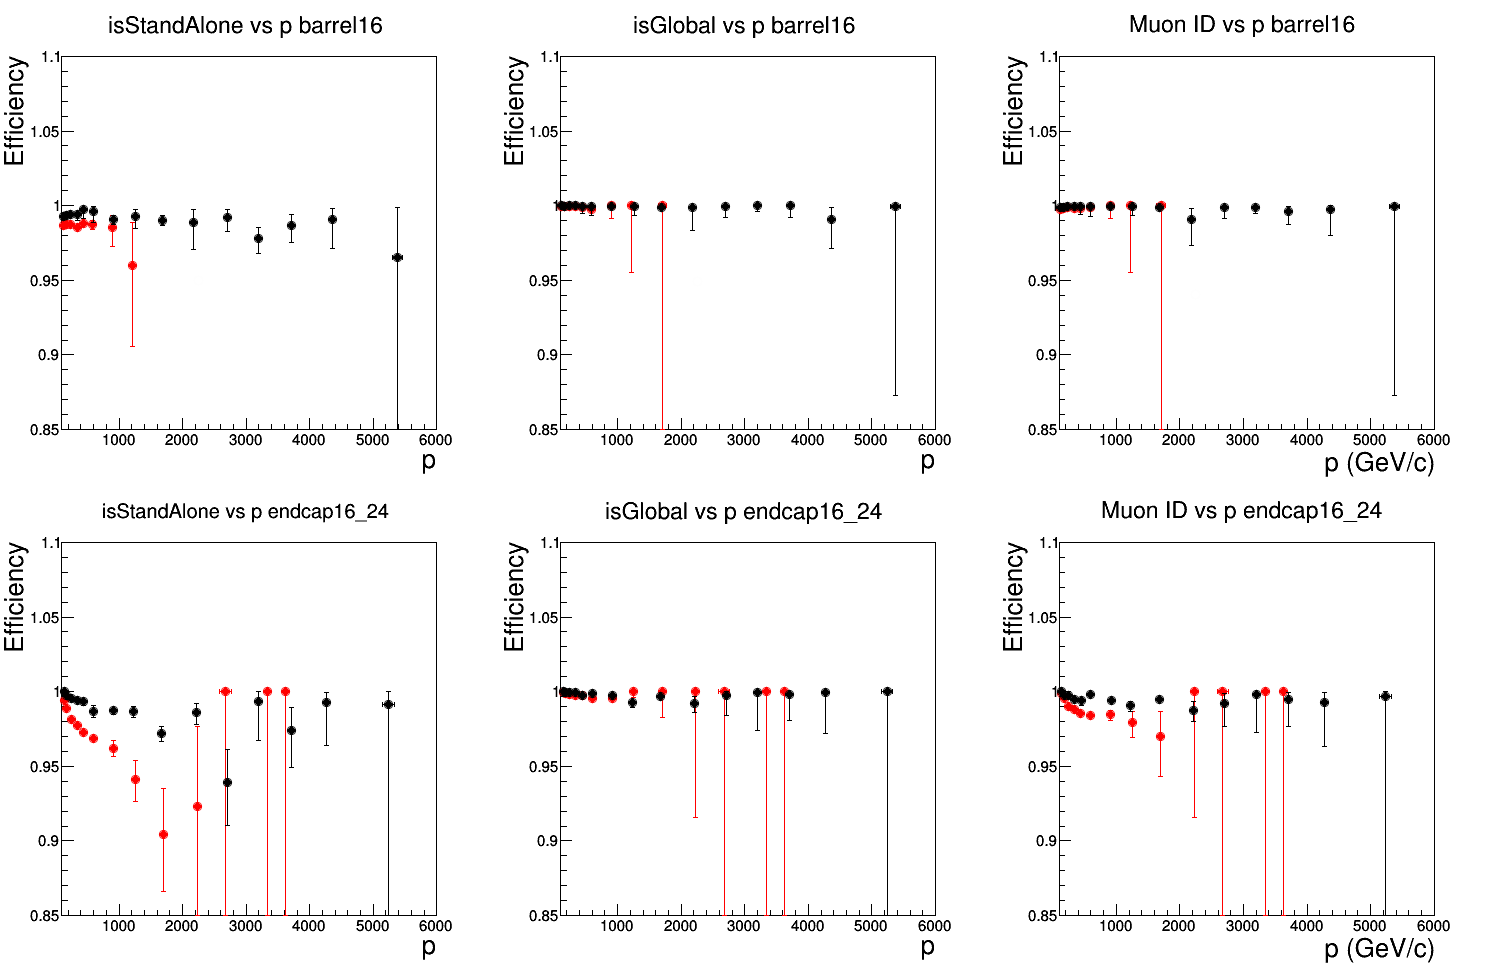
\includegraphics[width=0.85\textwidth]{Images/Cap5/Fit_Standalone.png}
\caption{Factorized muon reconstruction and identification efficiency as a function of muon momentum in barrel up to 1.6 (top raw) and endcap between 1.6 and 2.4 (bottom raw): the red points represent the data, while the black points represent the MC. The pure Standalone reconstruction efficiency is plotted on the left, the Global reconstruction efficiency calculated w.r.t. the probes passing also the Standalone is plotted in the middle, and the MuonID efficiency calculated w.r.t the probes passing the Global reconstruction is plotted on the right.}
\label{fig_reco_s}
\end{figure}

\begin{comment}
Therefore to asses the robustness of this study, and to conclude that the MC is not properly describing the data at high momentum, it has been checked if the tracker weak mode, causing a bad momentum measurement, can bias the result. The weak mode is due to the tracker alignment and affects only the data. It would give a different efficiency as a function of phi according to the charge. It is present only in the endcap, and it differently affects the negative and the positive endcap regions. The plots in figure~\ref{fig_weakmode1} show the efficiency as a function of phi for the positive and the negative endcap (top and bottom raw respectively) comparing positive (in green) and negative (in blue) muons. The efficiency has been calculated starting from different momentum values. Despite some differences are present, there is not any effect of the weak mode. As a double check the efficiency summing positive and negative muons has been calculated and compared to the same from MC (figure~\ref{fig_weakmode2}). The conclusion is that the discrepancy between data and MC doesn't have any extra dependence on phi related to the tracker weak mode. 

Another test has been done adding the kinematic cuts to Tag and Probe selection: 
\begin{itemize}
\item $p^{1}_{T}/p^{2}_{T} < 3$ 
\item $\Delta{\phi}(\mu^{1}\mu^{2}) > 2.5$
\end{itemize}

No relevant changes have been observed. 

Also the scanning of the events has been done, at least for those at high momentum. It is visible from the event displays that the presence of electromagnetic shower is a common feature for the probe muons failing the reconstruction.  
\end{comment}

Comparing data and simulation, there is a clear effect depend from the muon momentum so the introduction of a systematic error varying with the muon momentum and the eta region is needed. This scale factor is then used to get a weight for each muon according to its momentum. This weight is divided for a reference value which corresponds to the weight at $p = 100$ GeV in the barrel and a weight at $p = 200$ GeV in the endcap. This is done to take into account the scale factor calculated at Z peak, already applied in the analysis, which has not to be double counted. The difference on the mass distribution obtained by reweighting or not the events is than taken as systematic.  

%The systematic error is differently calculated for the barrel up to 1.6 and for the endcap between 1.6 and 2.4. In the first region, since the data prefer a constant function while the MC is better described by a linear function, the MC efficiency is directly taken as scale factor ((figure~\ref{fig_reco_f}) bottom left). In the endcap, where both data and MC efficiencies are described by a linear function, the ratio of the two is taken as scale factor (figure~\ref{fig_reco_f} bottom right).  
\begin{comment}
\begin{figure}[htbp]
\centering
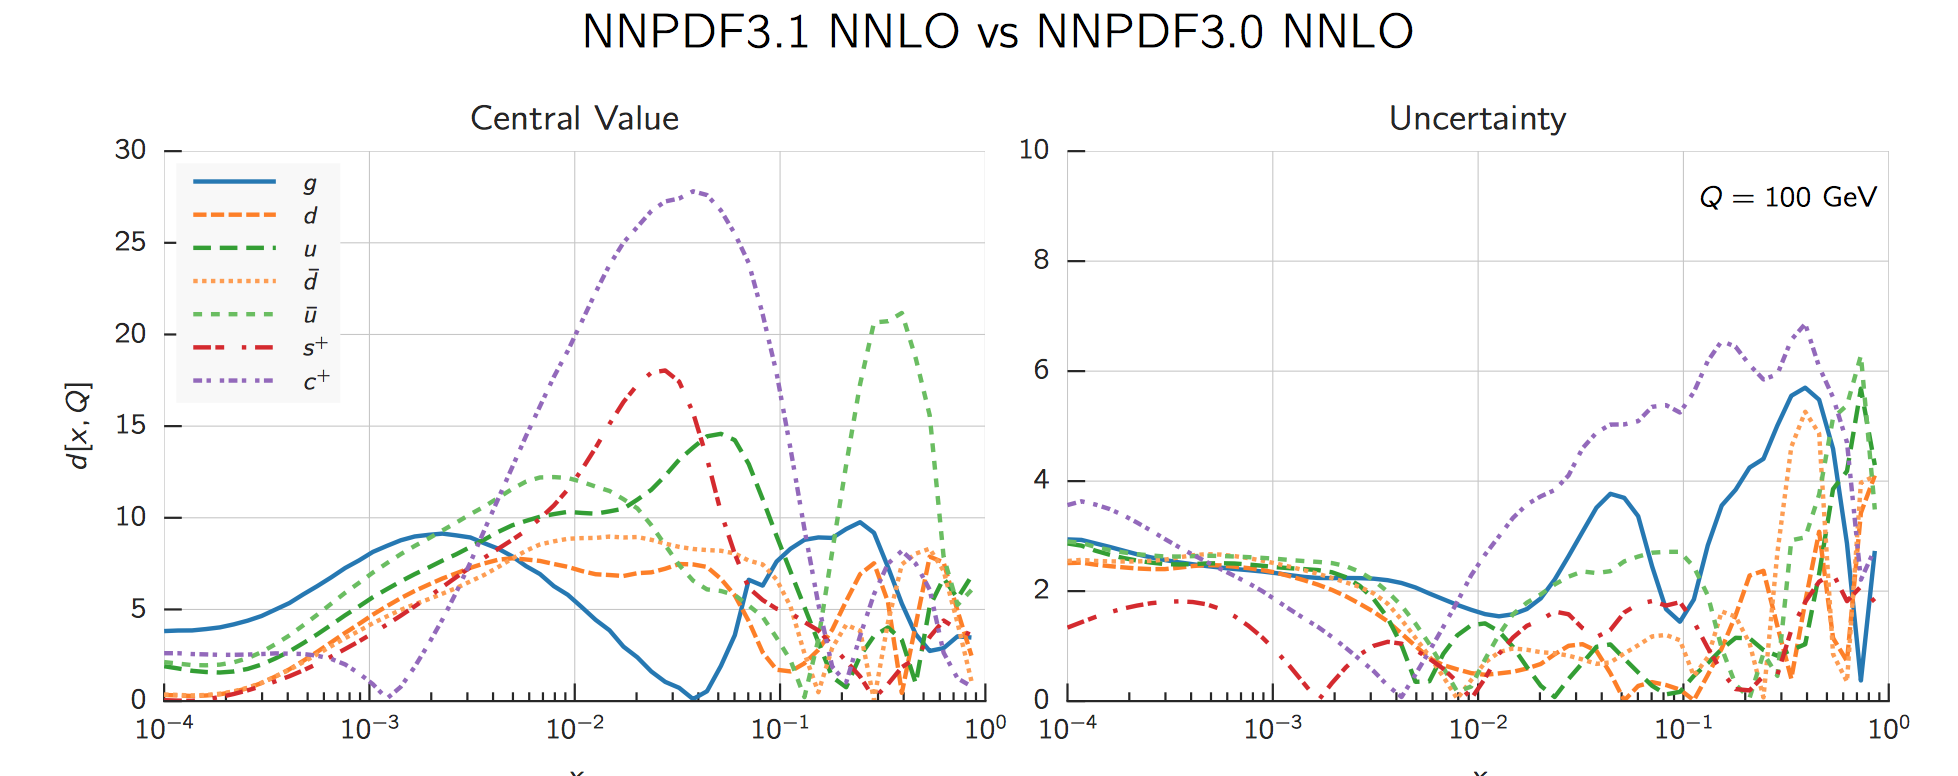
\includegraphics[width=0.1\textwidth]{Images/NNPDF_30_31}
\caption{Muon reconstruction and identification efficiency as a function of phi for different momentum thresholds: on top is the positive endcap from 1.6 up to 2.4, at the bottom is the negative endcap from -1.6 up to -2.4. The blue points represent the positive muons, while the green points represent the negative muons. The columns are relative to the muon momentum threshold: all p, 300 GeV, 450 GeV, 650 GeV. The plots show only the data.}
\label{fig_weakmode1}
\end{figure}

\begin{figure}[htbp]
\centering
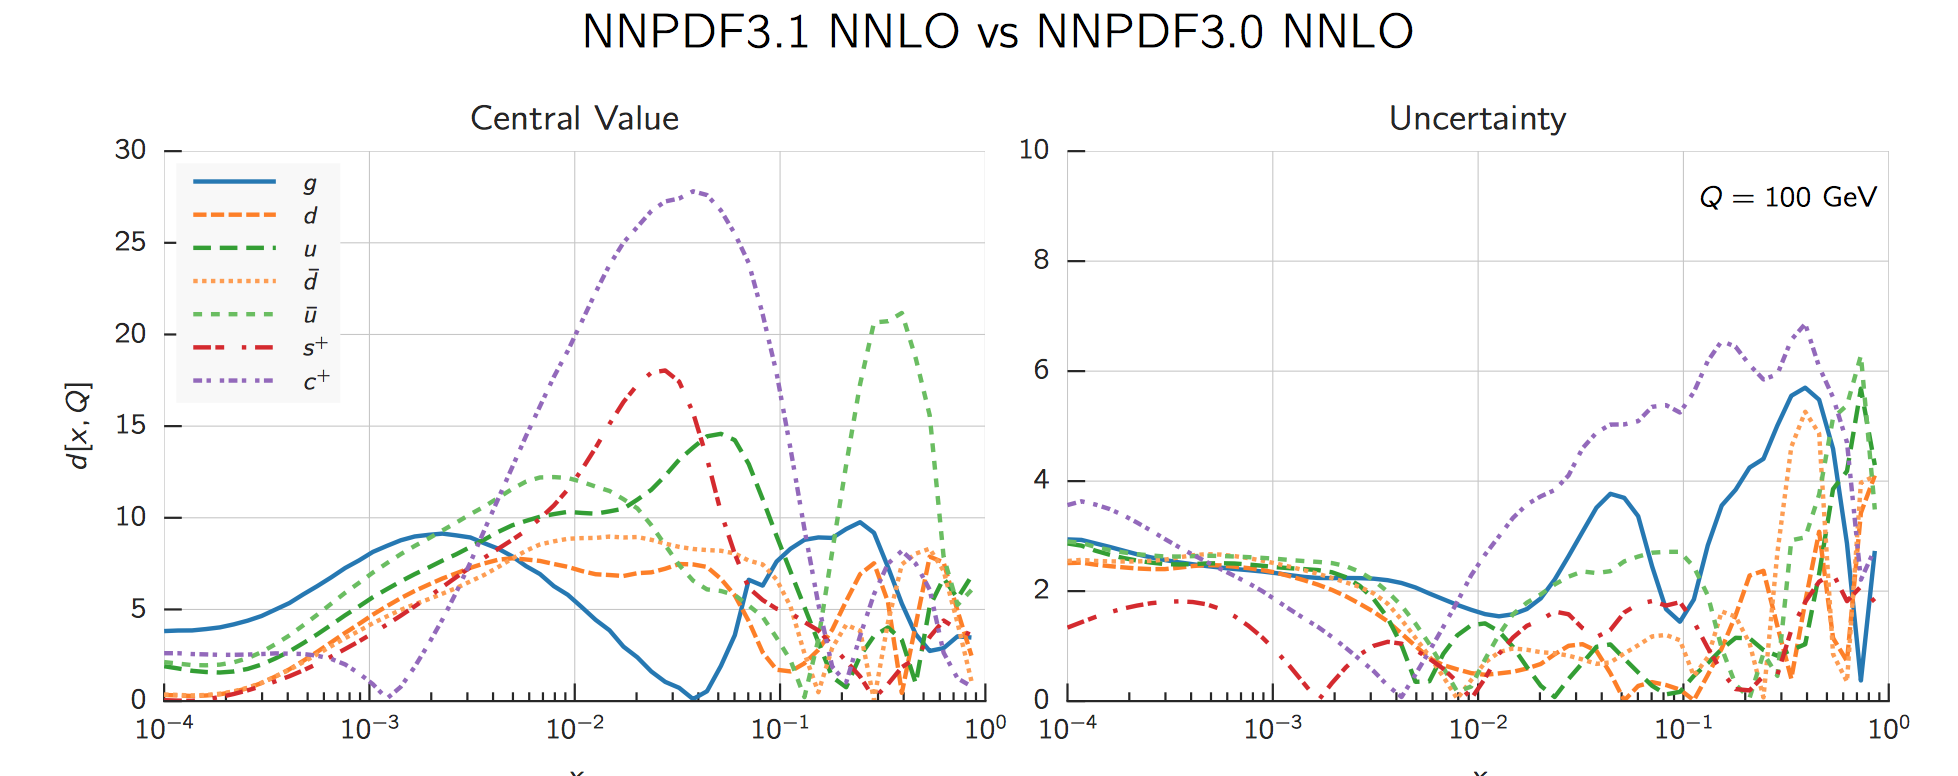
\includegraphics[width=0.1\textwidth]{Images/NNPDF_30_31}
\caption{Muon reconstruction and identification efficiency as a function of phi for different momentum thresholds summing positive and negative muons: on top is the positive endcap from 1.6 up to 2.4, at the bottom is the negative endcap from -1.6 up to -2.4. The red points represent the data, while the black points represent the MC. The columns are relative to the muon momentum threshold: all p, 300 GeV, 450 GeV, 650 GeV. The plots show only the data.}
\label{fig_weakmode2}
\end{figure}

\begin{figure}[htbp]
\centering
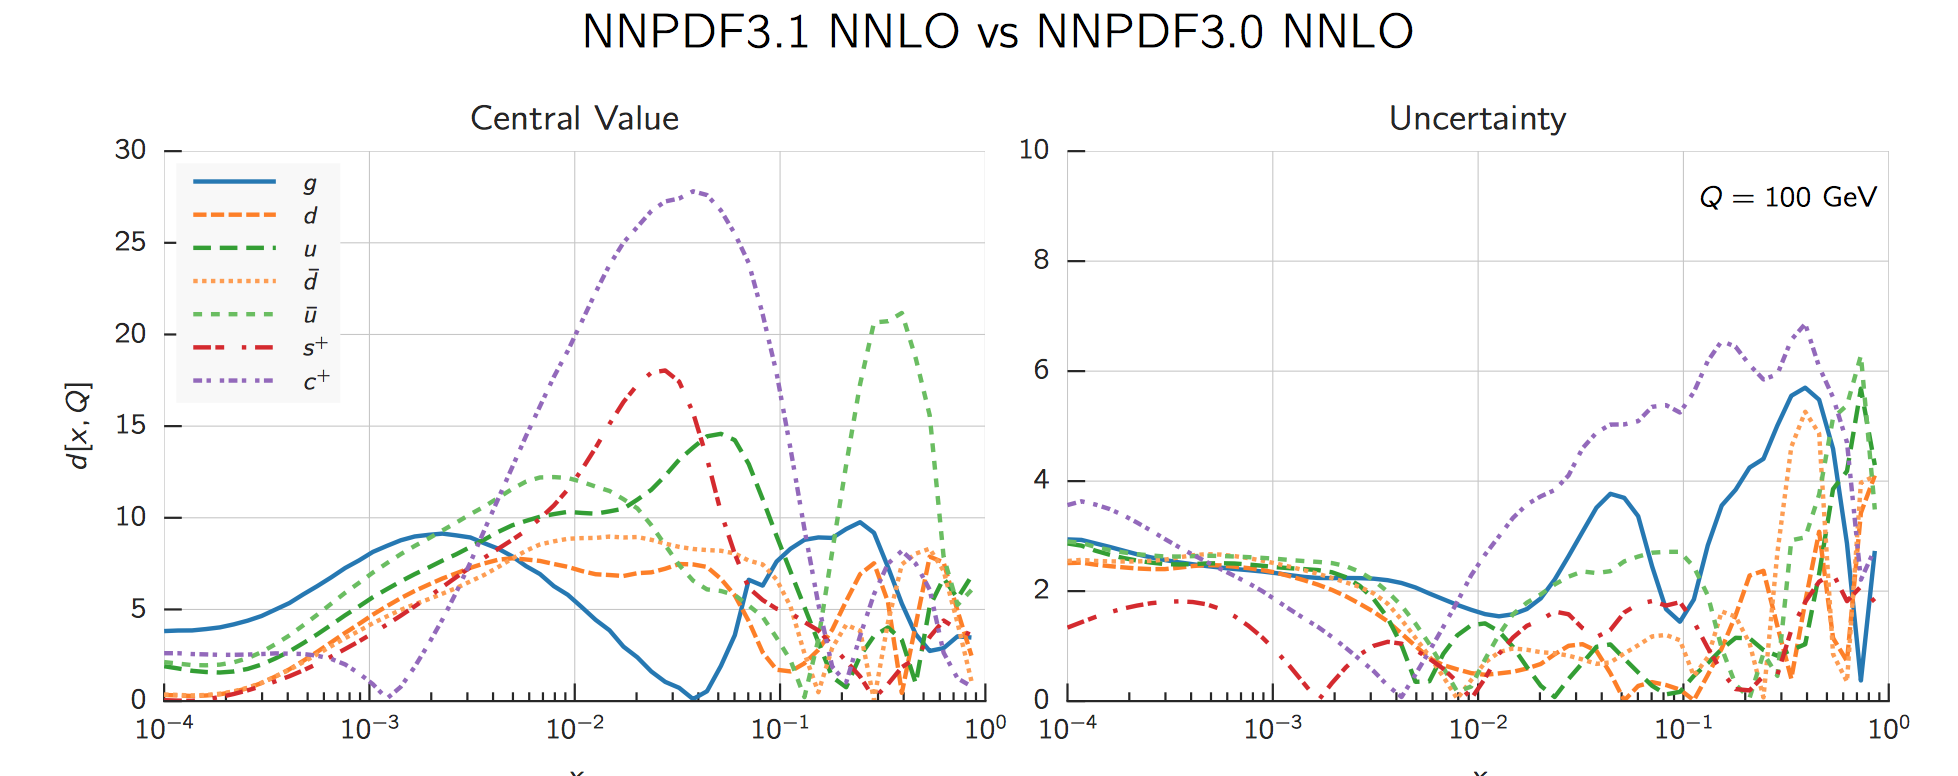
\includegraphics[width=0.1\textwidth]{Images/NNPDF_30_31}
\caption{Muon reconstruction and identification efficiency as a function of muon momentum in barrel up 1.6 (top left) and endcap between 1.6 and 2.4 (top right): the red points represent the data, while the black points represent the MC. Data and MC are interpolated by a first order polynomial. The fits are performed starting from 150 GeV in the barrel and 300 GeV in the endcap, up to 2000 GeV for data and up to 6000 GeV for MC. The boxes report the fit parameters. In bottom are the scale factors used to estimate the systematic uncertainty: on the left the scale factor is taken as the linear function describing the MC efficiency, while on the right the scale factor is calculated as the ratio of the functions describing the Data and MC efficiencies.}
\label{fig_reco_f}
\end{figure}
\end{comment}

\section{Muon selection}
\label{sec:selection}
Muon selection (denoted as High-pT selection \ref{sec:Identification}) is set following the recommendation gave by the MuonPOG \cite{MuonPOG}:
\begin{itemize}
%\item  To avoid events from beam backgrounds, we filter out events in which fewer than a quarter of the tracks in the silicon tracker are marked as being of high purity.
\item a good offline-reconstructed primary vertex (PV) is required to be found in the event, as defined by the tracking POG: at least four tracks must be associated to the vertex and the vertex must be located within $|r| <$ 2 cm and $|z|<$ 24 cm of the nominal interaction point (IP). This cut has been established to ensure the quality of the hadronic collisions and discard detection of particles produced between beam particles and residuals present in the imperfect vacuum of LHC. On top of that, this cut allows to reject cosmic ray muons triggering in empty bunch-crossings, which can produce fake dimuons when traversing the detector near the IP.
\item the muon must be reconstructed as a global muon and a tracker muon (see section \ref{sec:Reconstruction}).
\item the offline muon \pt must be at least 53 GeV, so as to be in the plateau of the single- muon trigger efficiency (\textbf{AGGIUNGI EFFICIENCY TIRGGER SINGLE MU DOVE SI VEDE IL PLATEAU})
\item the relative \pt error $\delta$\pt / \pt is required to be smaller than 0.3, to suppress grossly mismeasured muon tracks and especially ensure the quality of the \pt measurement.
\item the muon's transverse impact parameter with respect to the primary vertex, as measured by the tracker-only fit, must be less than 0.2 cm.
\item the muon must pass a relative tracker-only isolation cut: the scalar sum of the \pt of all other tracks in a cone of $\Delta R = \sqrt{\Delta\eta^2 + \Delta\phi^2} <$ 0.3 around but not including the muon's tracker track must be less than 10\% of the muon's \pt, also as measured by the tracker. To be used in the calculation of the tracker isolation, tracks have to be within $\Delta z$ = 0.2 cm of the primary vertex with which the muon candidate is associated.
\item the global muon track must have at least 6 tracker layers with hits in the fit.
\item the global muon track fit must include at least one hit from each of the pixel detector and the muon system.
\item the tracker muon must be matched to segments in at least one muon station if the muon station is not on the first layer of the muon system, or if matched to one muon station on the first layer we also require that the muon matches to more than two RPC layers, or that the muon is matched in at least two muon stations. 
\end{itemize}
To form a dimuon, two muons of opposite charge passing the above selection have been considered. A fit to a common vertex (using the Kalman filter formulation) has been performed to compute the kinematics of the dimuon system, particularly its invariant mass. This also serves to ensure that the two muons originate from the same vertex, as a safety check against pile-up and as a check on reconstruction quality; we explicitly require that the vertex fit has $\chi^2$ /d.o.f. $<$ 20. To reduce the background from cosmic ray muons that are in-time with a collision event and pass the primary vertex and impact parameter cuts, the three-dimensional angle between the two muons' momenta must be less than $\pi$ - 0.02 rad.\\
In events with more than one opposite-sign dimuon, the two muons with highest \pt sum are considered. \\

\subsection{Muon ID efficiency}
\label{sec:IDefficiency}
The Tag and Probe technique is also used to evaluate single muon efficiency. First the events must satisfy trigger conditions; then both the tag and probe must be global and tracker muon with \pt$>$ 53 GeV, $|\eta|<2.4$ and relative tracker isolation $<0.1$. Muons so selected must have opposite charge, share a normalised vertex with $\chi^2$ /d.o.f. $<$ 20 and must be separated by a distance of $\Delta R>0.4$; the condition on the 3D angle $<\pi-0.02$ is also imposed. The tag and the passing probe are also required to have: $|dB|<0.2$, at least 6 tracker layers with hits in the fit, at least one hit from each of the pixel detector and the muon system; relative \pt error $\delta$\pt / \pt is required to be smaller than 0.3. Both muons must also pass the muon matched station cut defined in section \ref{sec:selection}. \\
The ID efficiency as a function of \pt, $\eta$ and $\phi$ is shown in \figurename~\ref{fig:IDEffVsPt} and \figurename~\ref{fig:IDEffVsEtaPhi}. The drops observed around $|\phi|=1.5$ is compatible with the gaps formed when the BPix layer was inserted in 2015.

\begin{figure}[htbp]
\centering
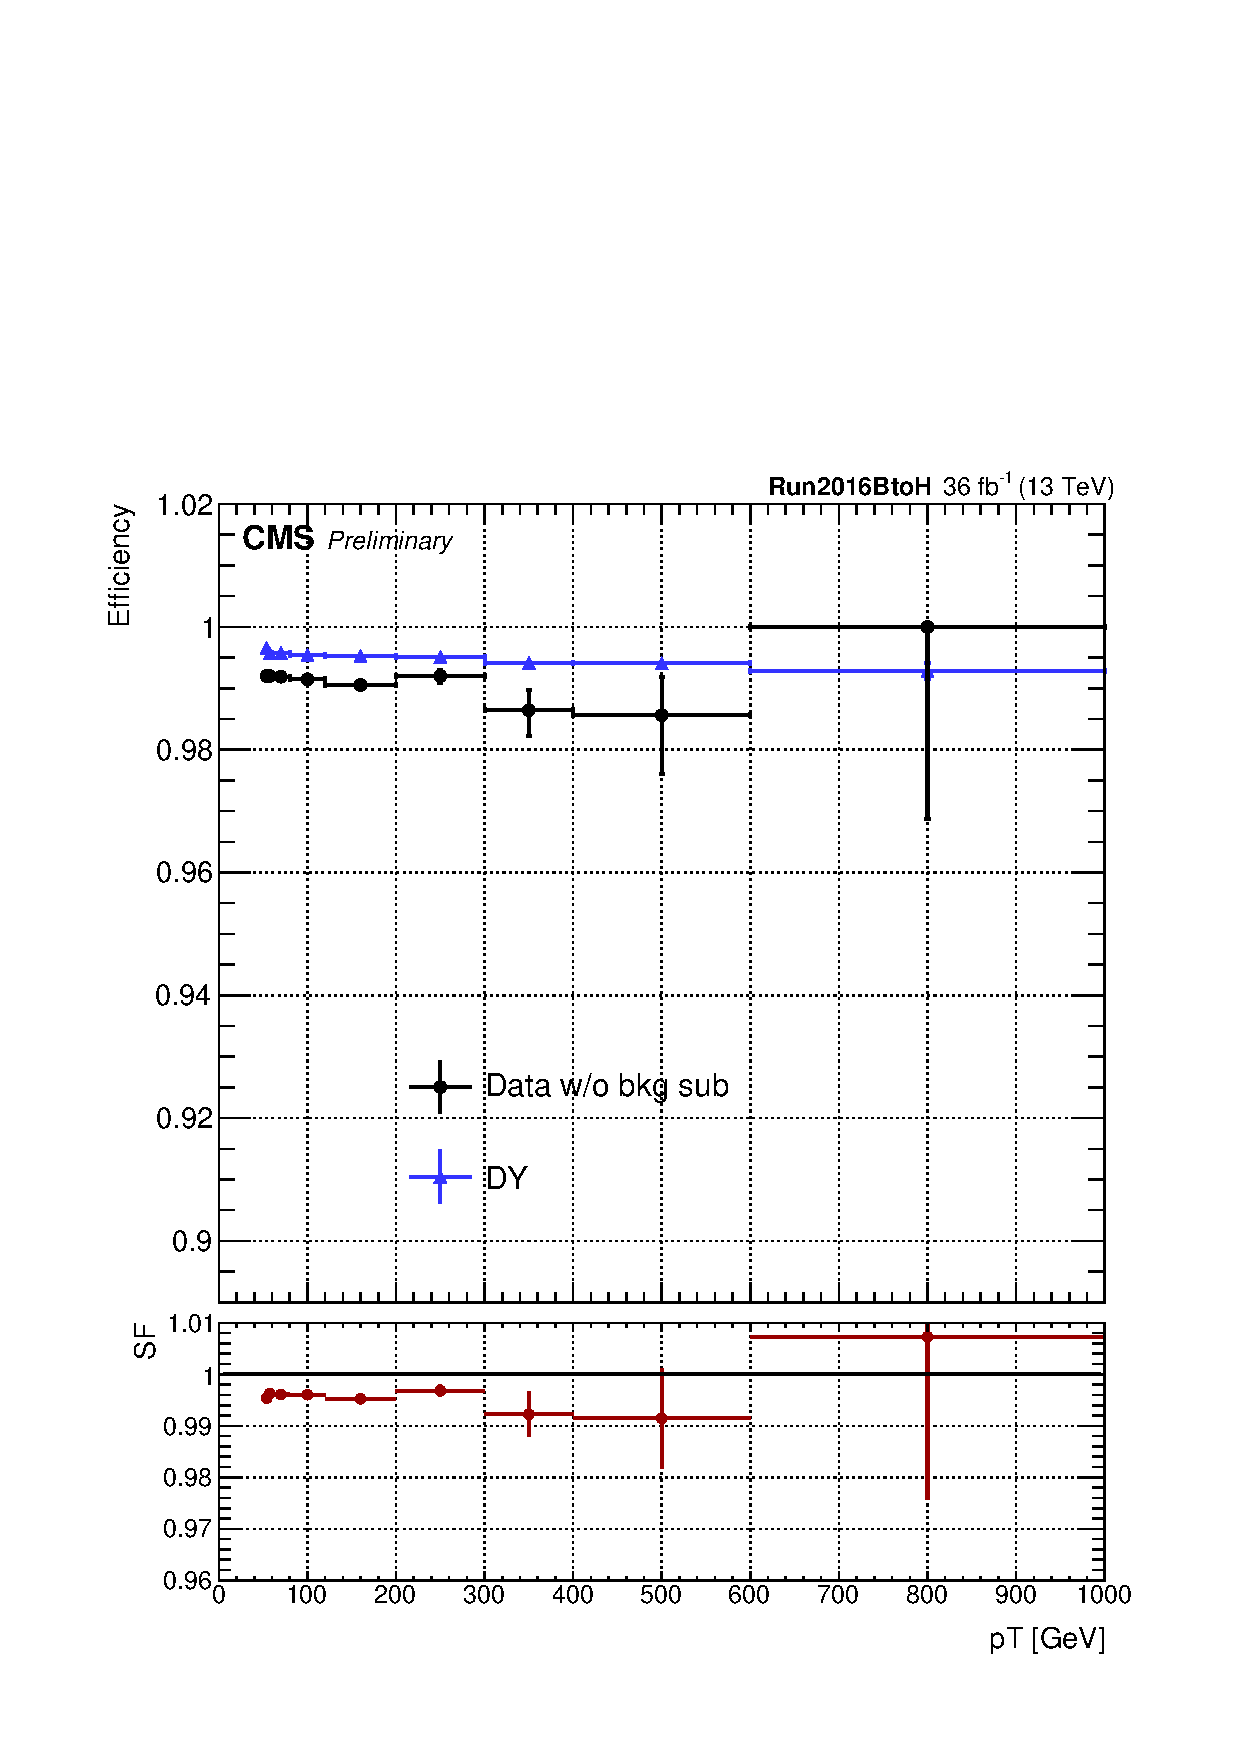
\includegraphics[width=0.45\textwidth]{Images/Cap5/Eff_FinalSel_Iso0p1_B2H_NoBkgSub_NoZwinNorm_Pt_B.pdf}
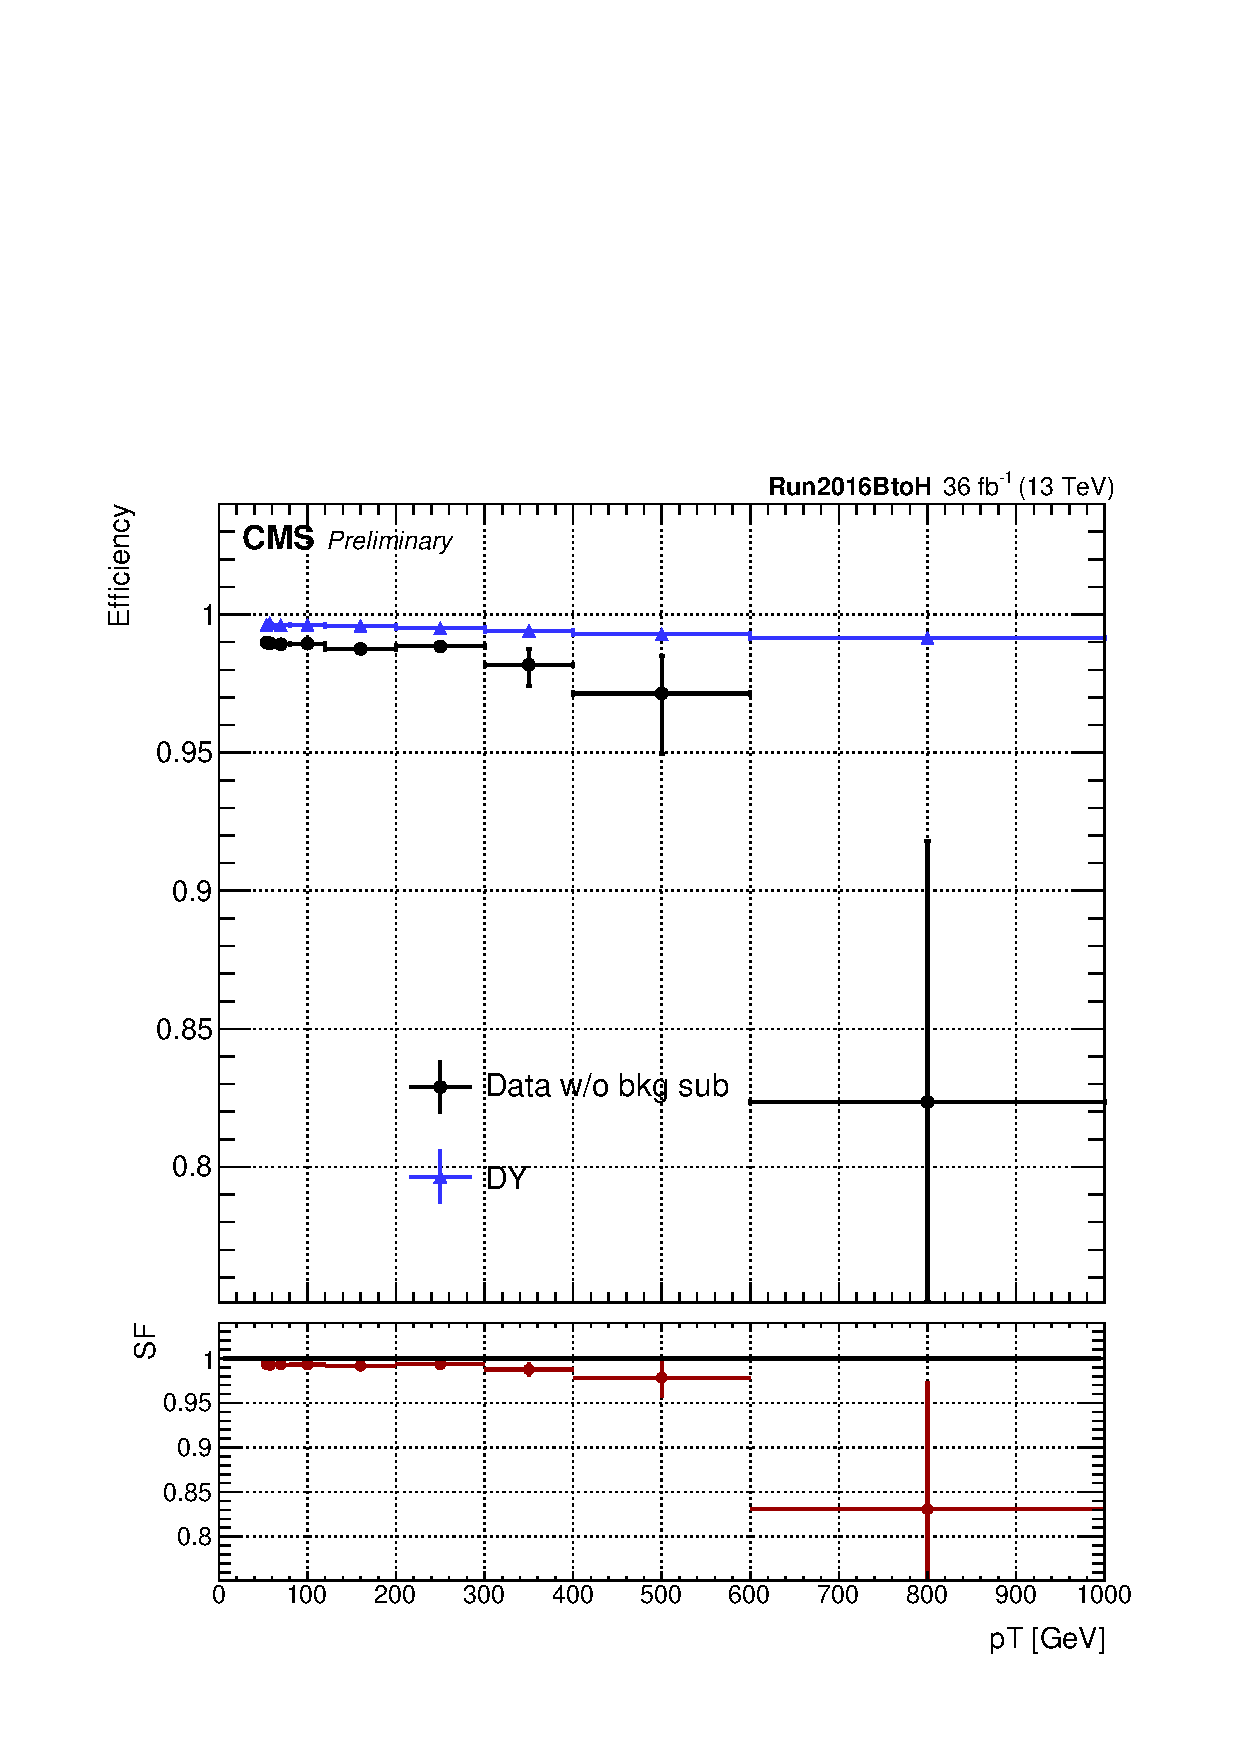
\includegraphics[width=0.45\textwidth]{Images/Cap5/Eff_FinalSel_Iso0p1_B2H_NoBkgSub_NoZwinNorm_Pt_E.pdf}
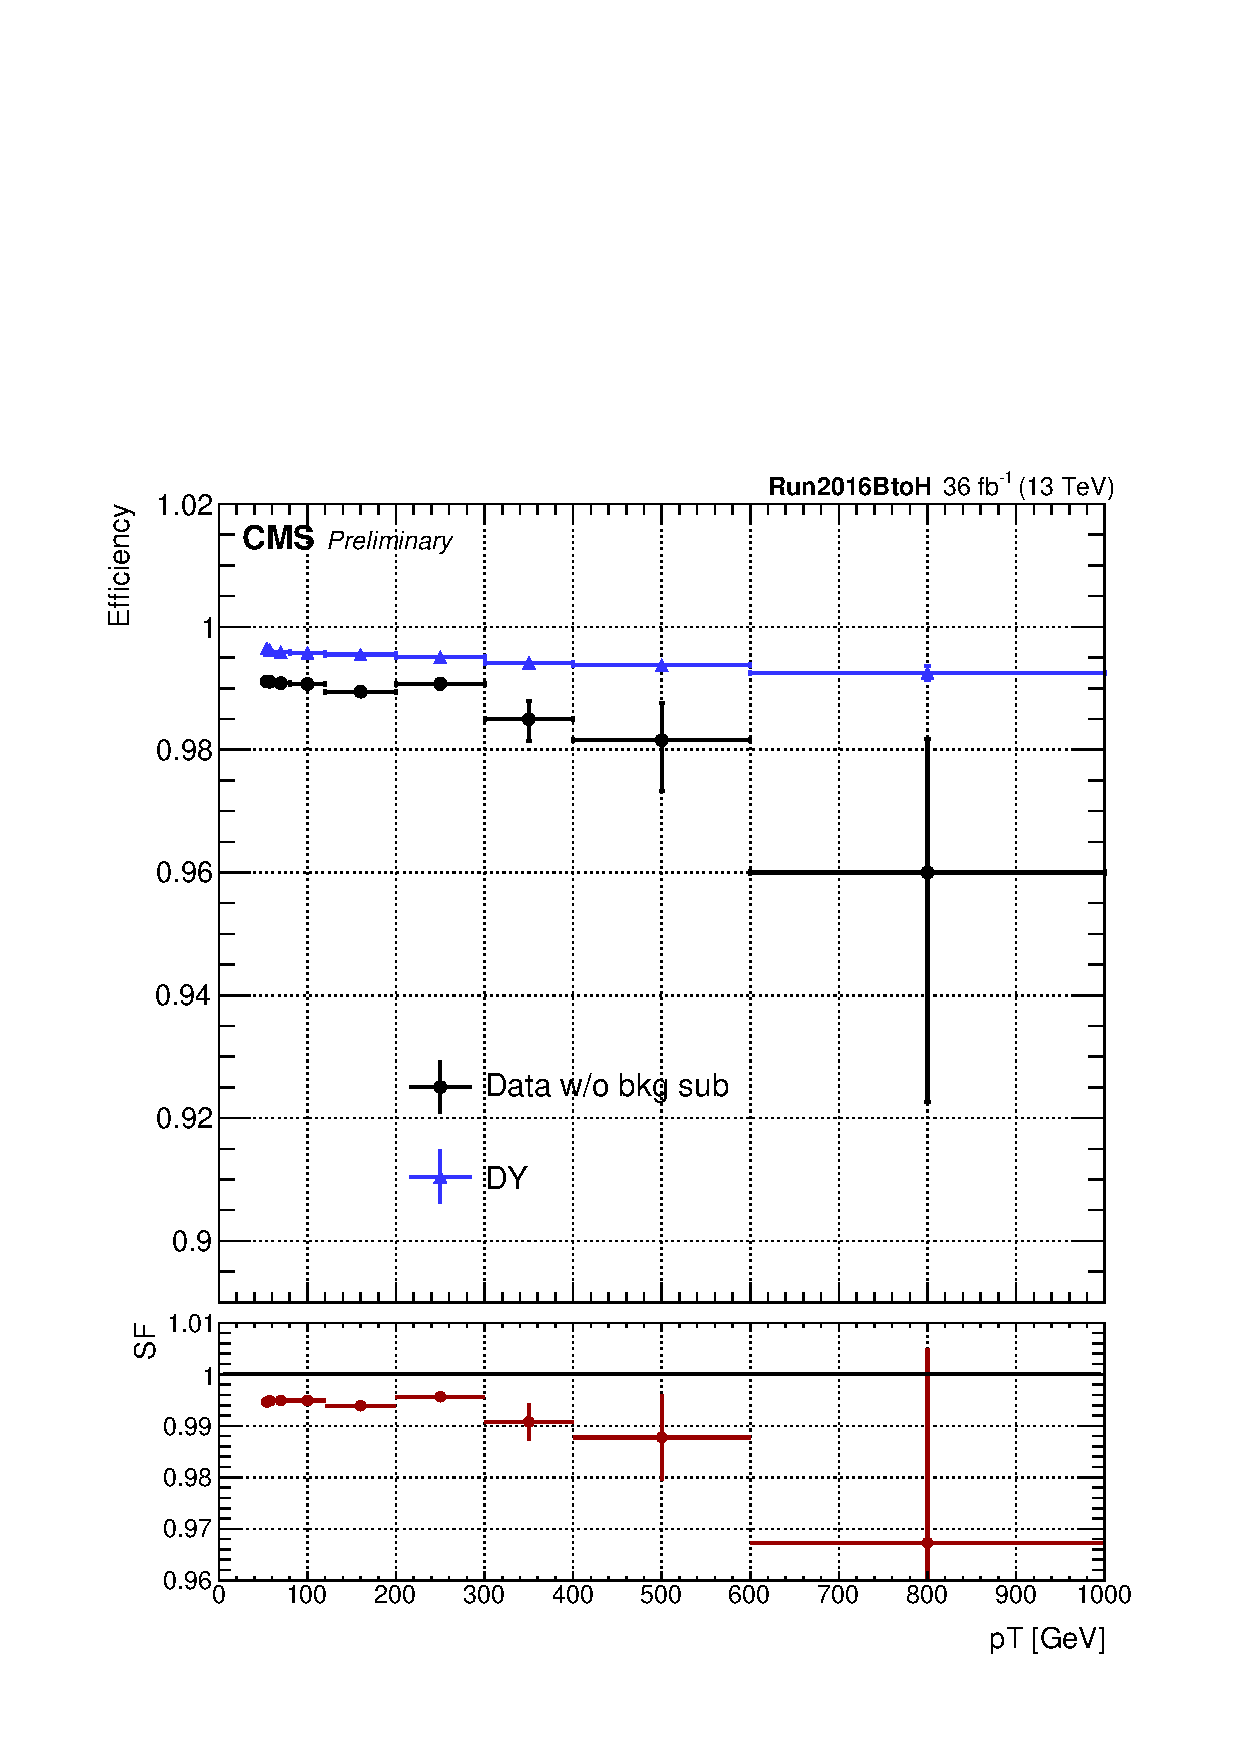
\includegraphics[width=0.45\textwidth]{Images/Cap5/Eff_FinalSel_Iso0p1_B2H_NoBkgSub_NoZwinNorm_Pt.pdf}
\caption{\label{fig:IDEffVsPt} The ID efficiency as measured using TuneP for 2016 Run as a function of muon \pt for only the barrel (left), only the endcaps (right), and all $\eta$ (Bottom).}
\end{figure}

\begin{figure}[htbp]
\centering
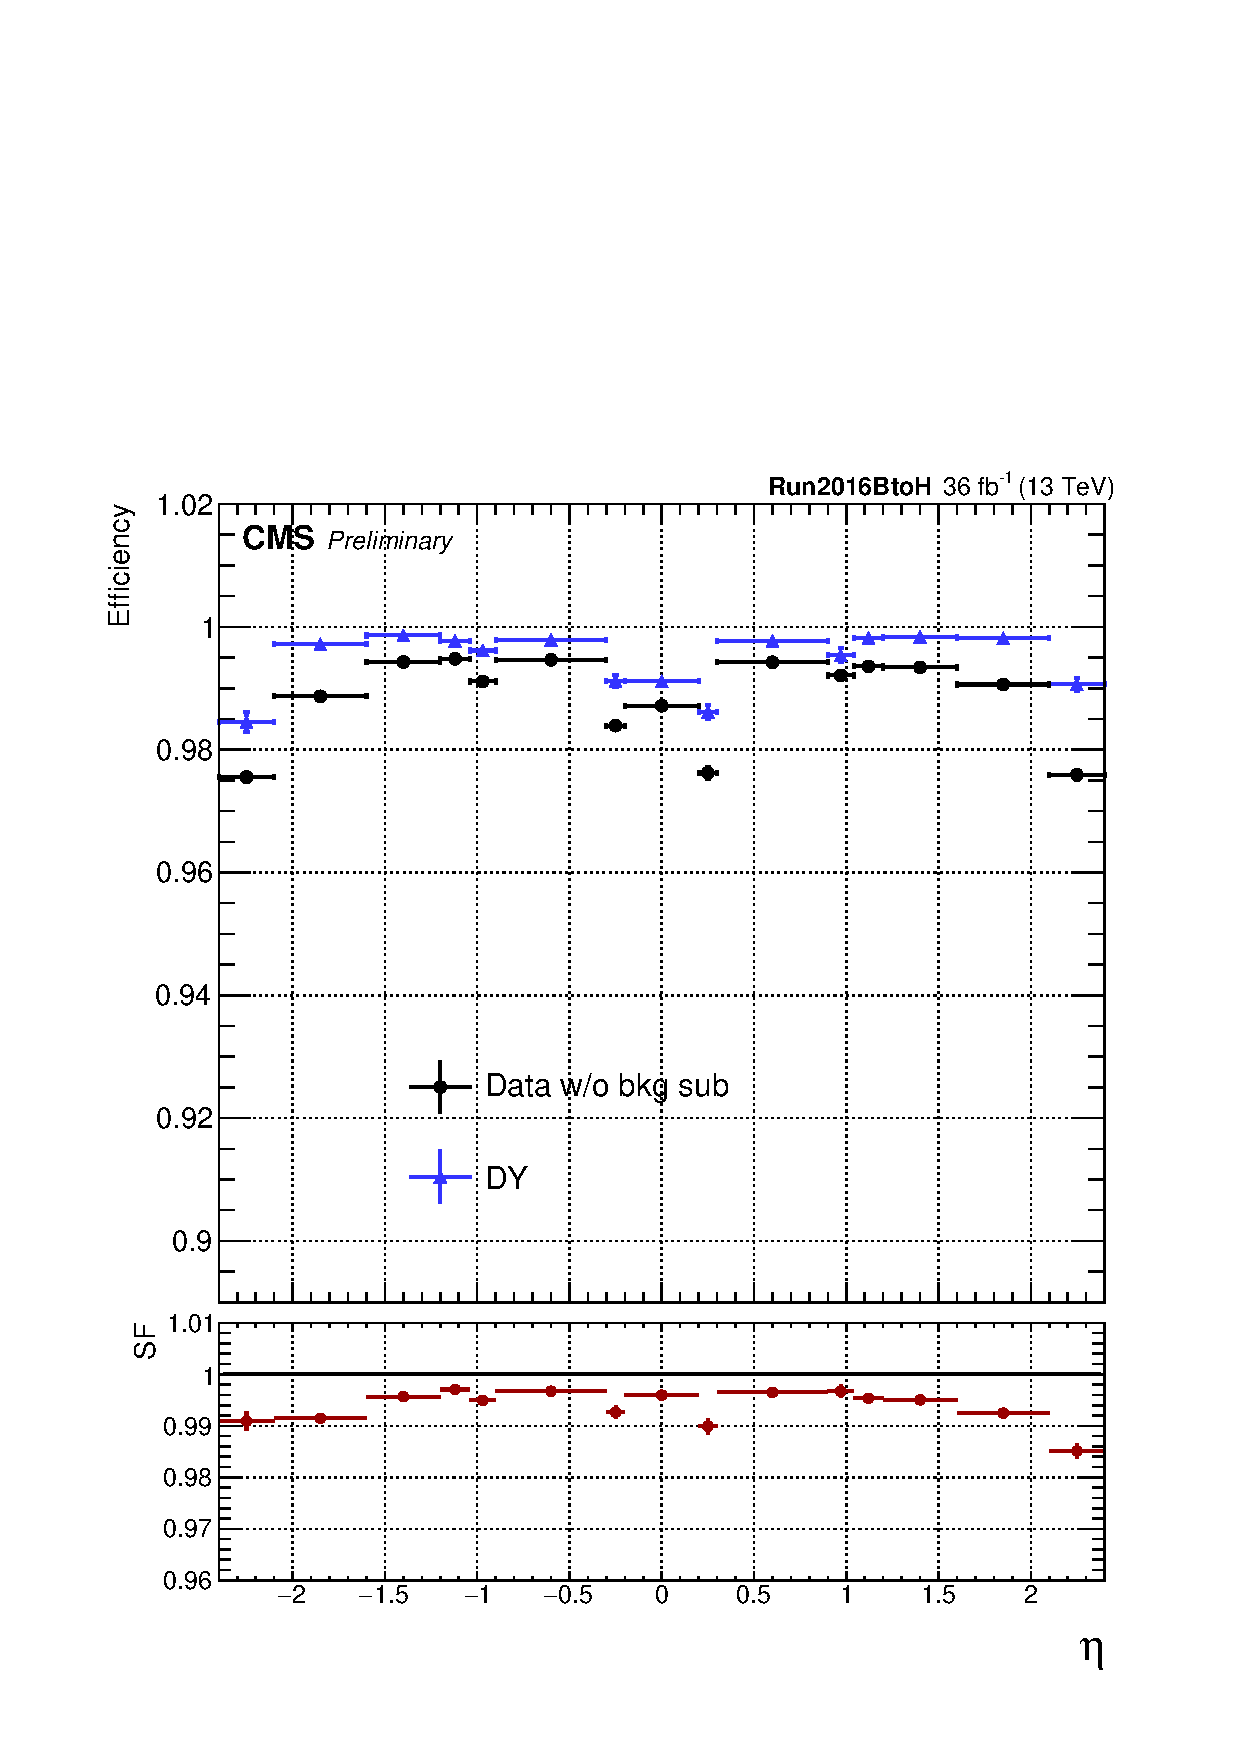
\includegraphics[width=0.45\textwidth]{Images/Cap5/Eff_FinalSel_Iso0p1_B2H_NoBkgSub_NoZwinNorm_Eta.pdf}
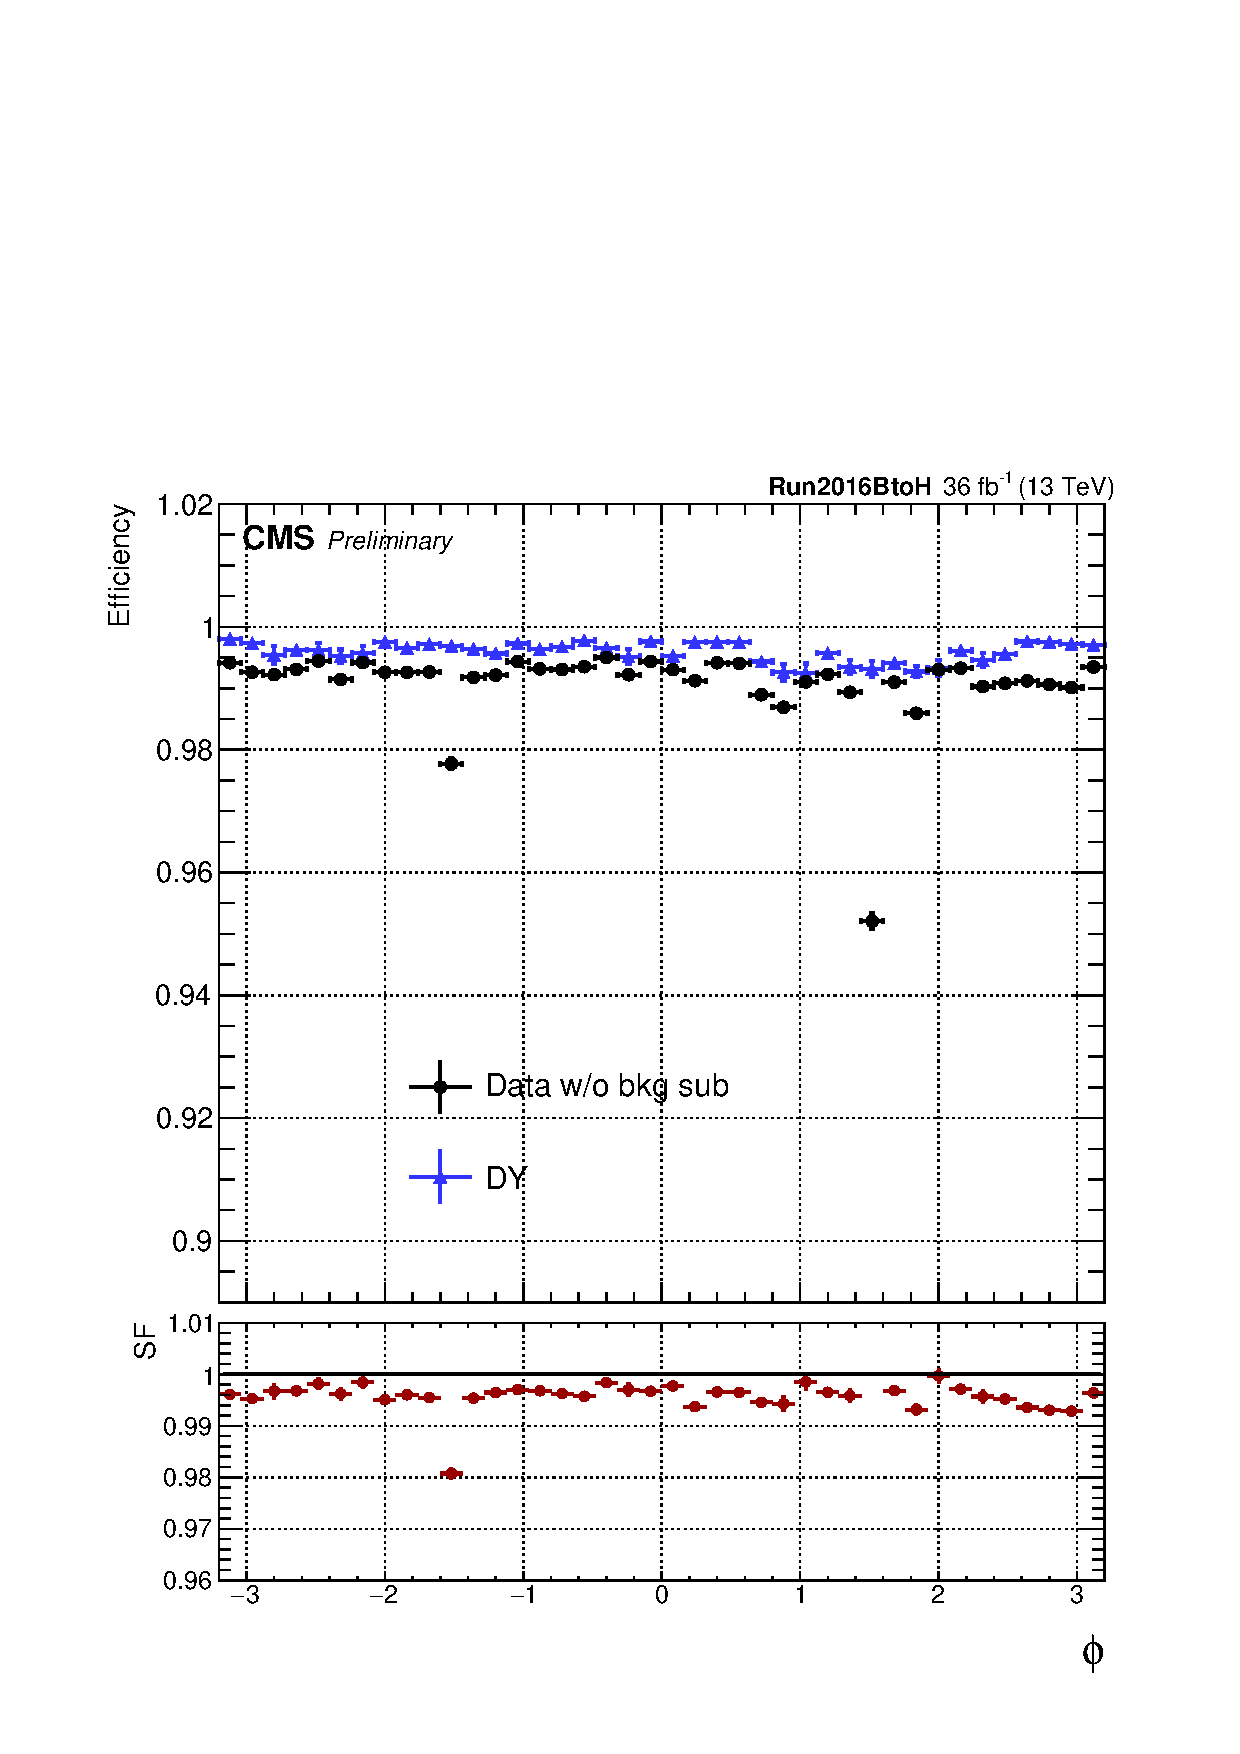
\includegraphics[width=0.45\textwidth]{Images/Cap5/Eff_FinalSel_Iso0p1_B2H_NoBkgSub_NoZwinNorm_Phi.pdf}
\caption{\label{fig:IDEffVsEtaPhi} The ID efficiency as measured using TuneP for 2016 Run as a function of muon $\eta$ (left) and muon $\phi$ (right).}
\end{figure}

The Scale Factor (SF) between data and MC associated is shown as a function of \pt in \figurename~\ref{fig:SFVsPt}.
\begin{figure}[htbp]
\centering
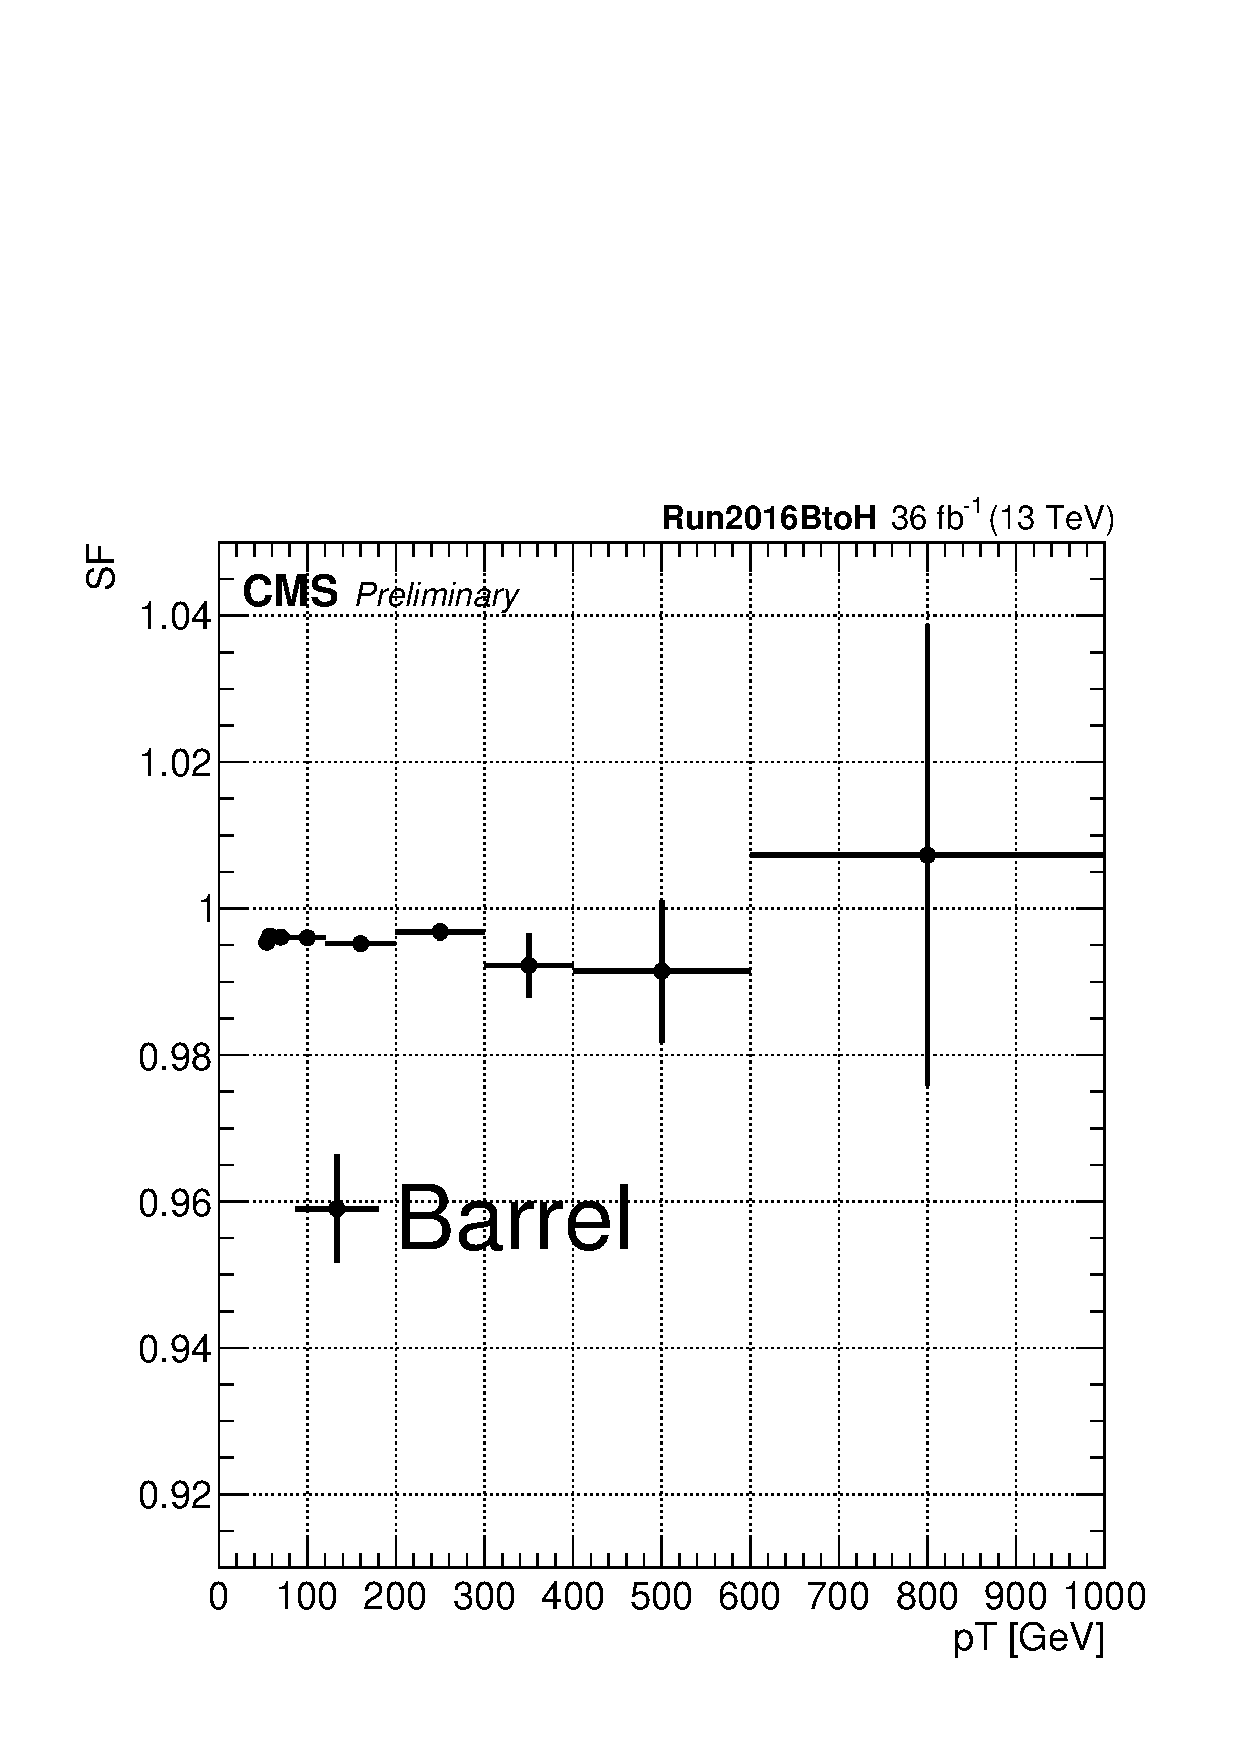
\includegraphics[width=0.45\textwidth]{Images/Cap5/FitSF_FinalSel_Iso0p1_B2H_Pt_B.pdf}
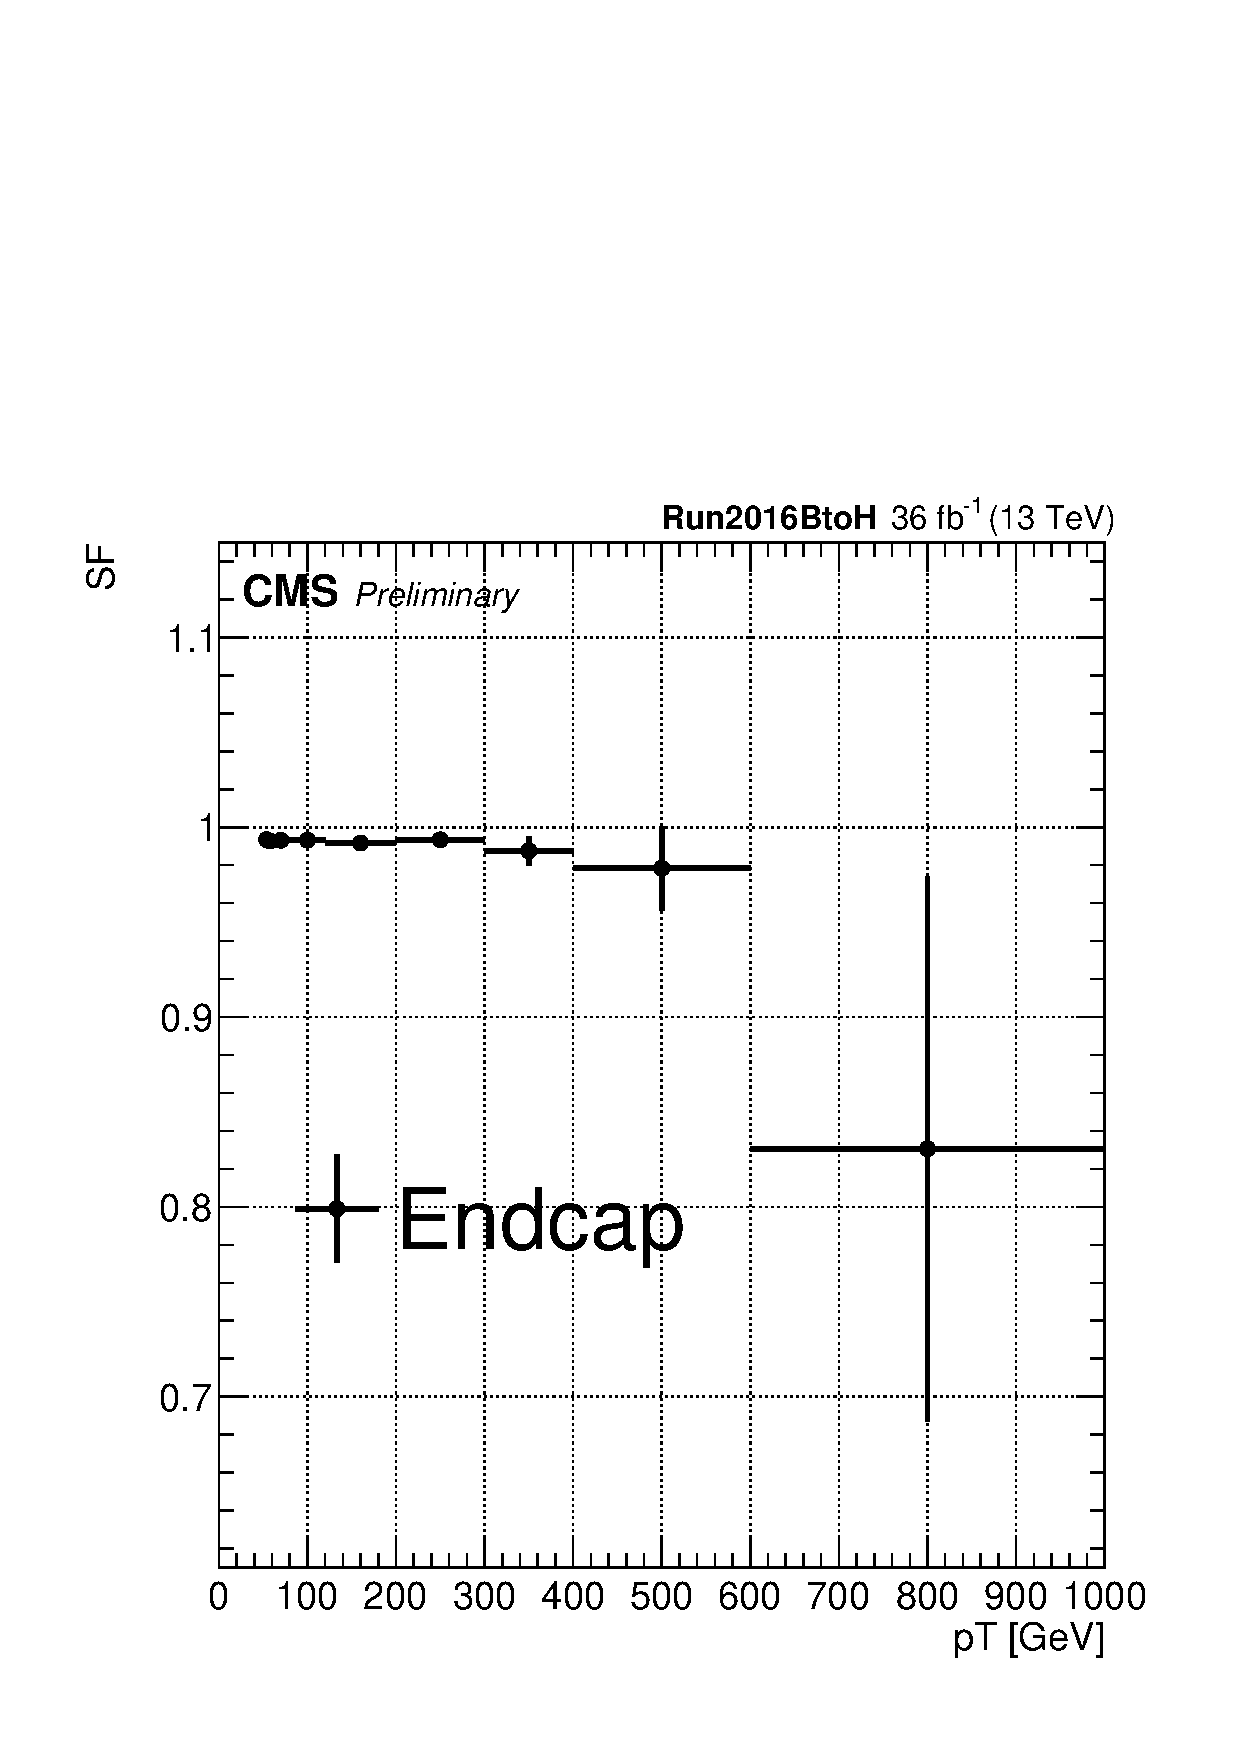
\includegraphics[width=0.45\textwidth]{Images/Cap5/FitSF_FinalSel_Iso0p1_B2H_Pt_E.pdf}
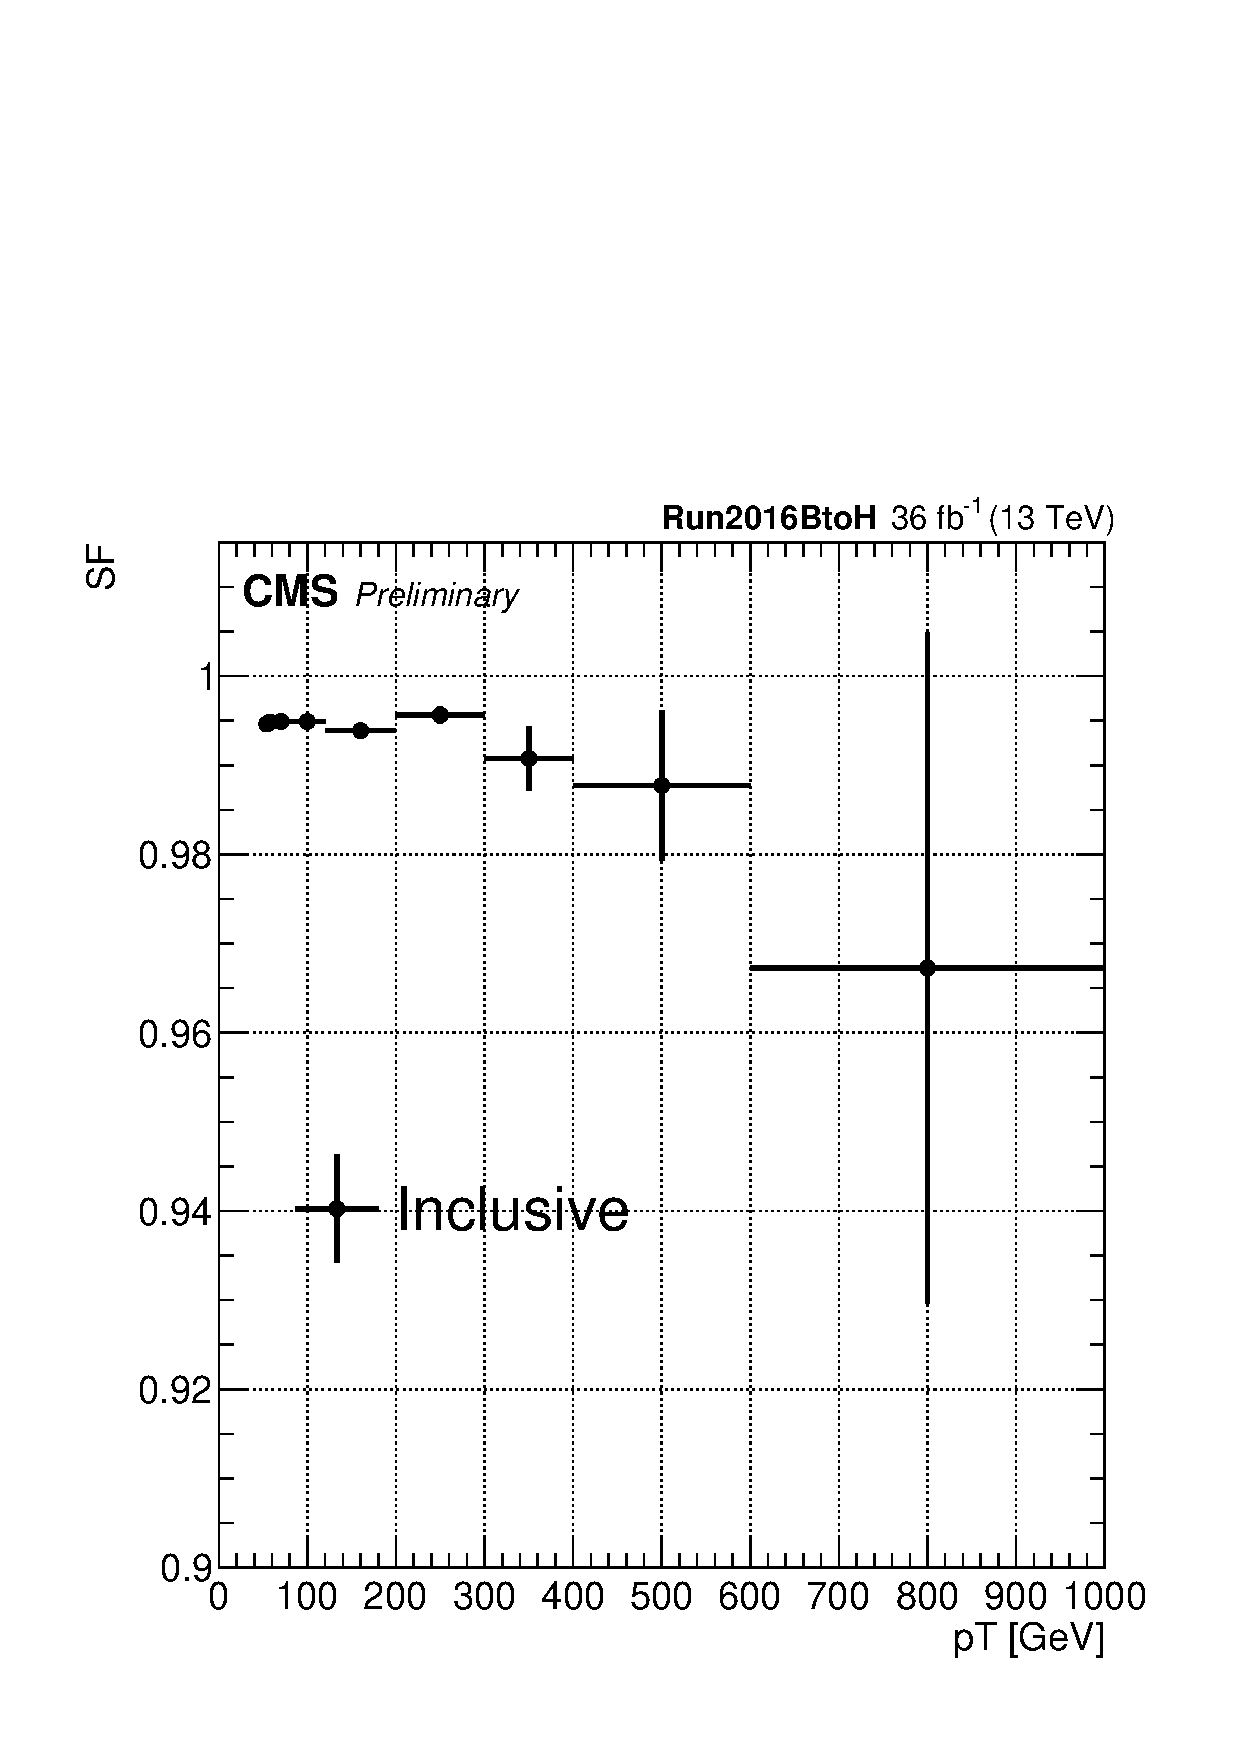
\includegraphics[width=0.45\textwidth]{Images/Cap5/FitSF_FinalSel_Iso0p1_B2H_Pt.pdf}
\caption{\label{fig:SFVsPt} The single muon efficiency Scale Factor for 2016 Run as a function of muon \pt for only the barrel (left), only the endcaps (right), and all $\eta$ (Bottom).}
\end{figure}

\begin{comment}
The efficiency of different ID selections were individually tested with respect to all other selections as N-1 plots.
\figurename~\ref{fig:IDEffNmO} shows the N-1 efficiencies for 2016 Run.
Two different selection criteria showed differences between data and MC; the number of pixel hits, and the number of muon hits.
Figures~\ref{fig:IDEffNmPixHitsVsPt} and~\ref{fig:IDEffNmMuoHitsVsPt} shows the N-1 efficiencies for these two selections as a function of muon \pt.
We see that these two selections do not vary more than 1\% as a function of muon \pt for the inclusive $\eta$ plots.

The dimuon ID efficiency is presented in Appendix~\ref{sec:dimuEff}.

\begin{figure}[htbp]
\centering
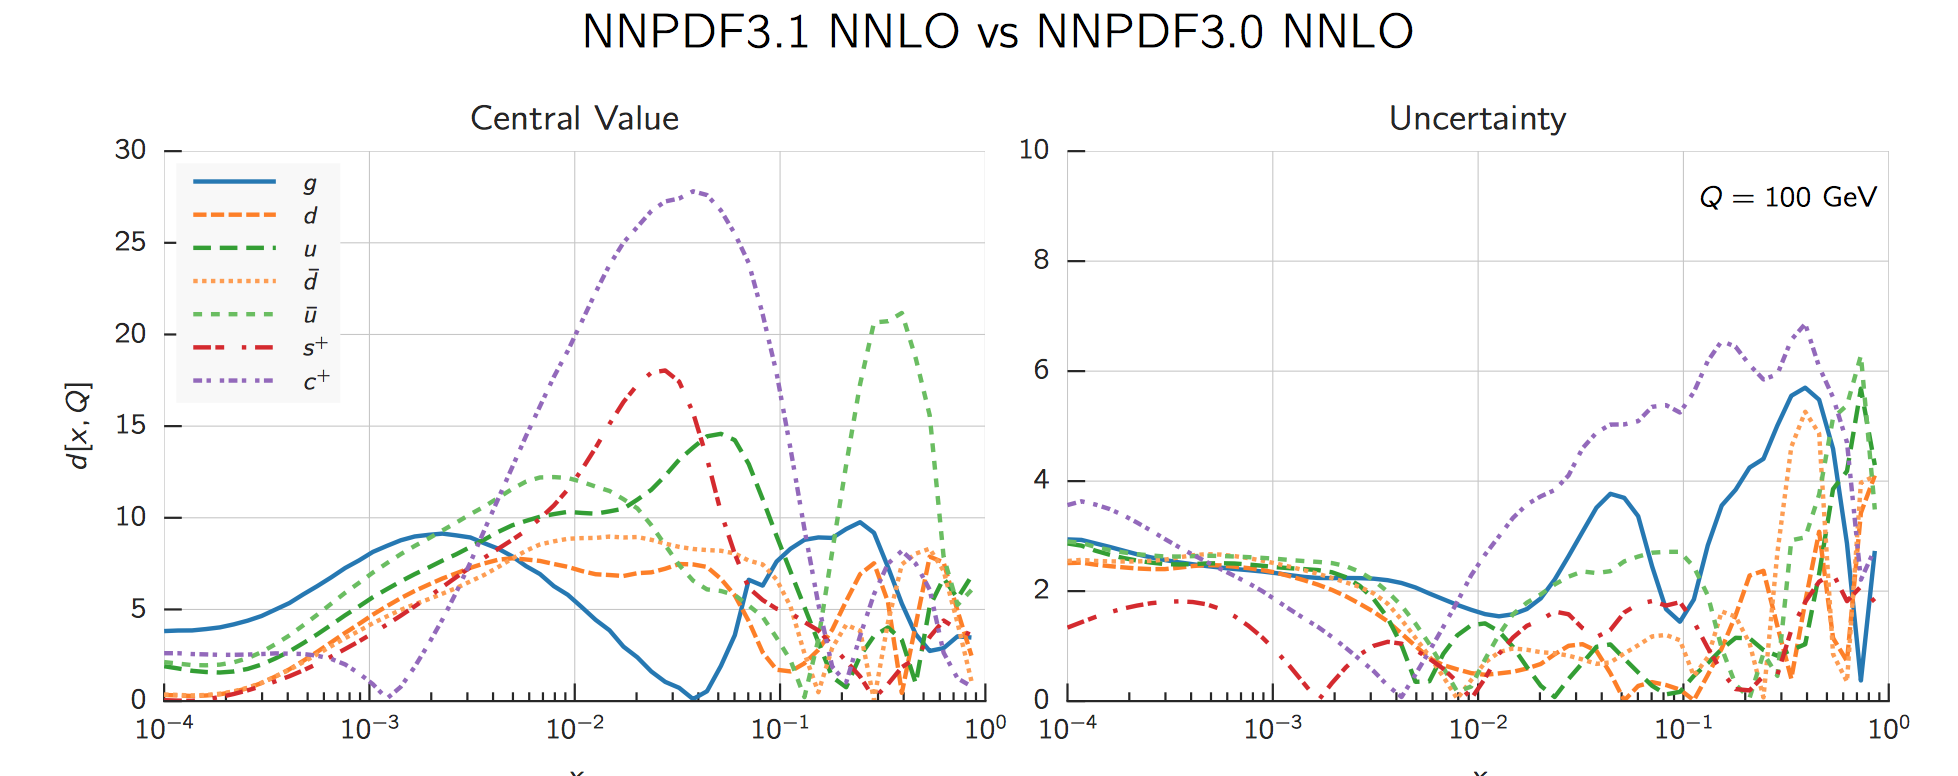
\includegraphics[width=0.1\textwidth]{Images/NNPDF_30_31}
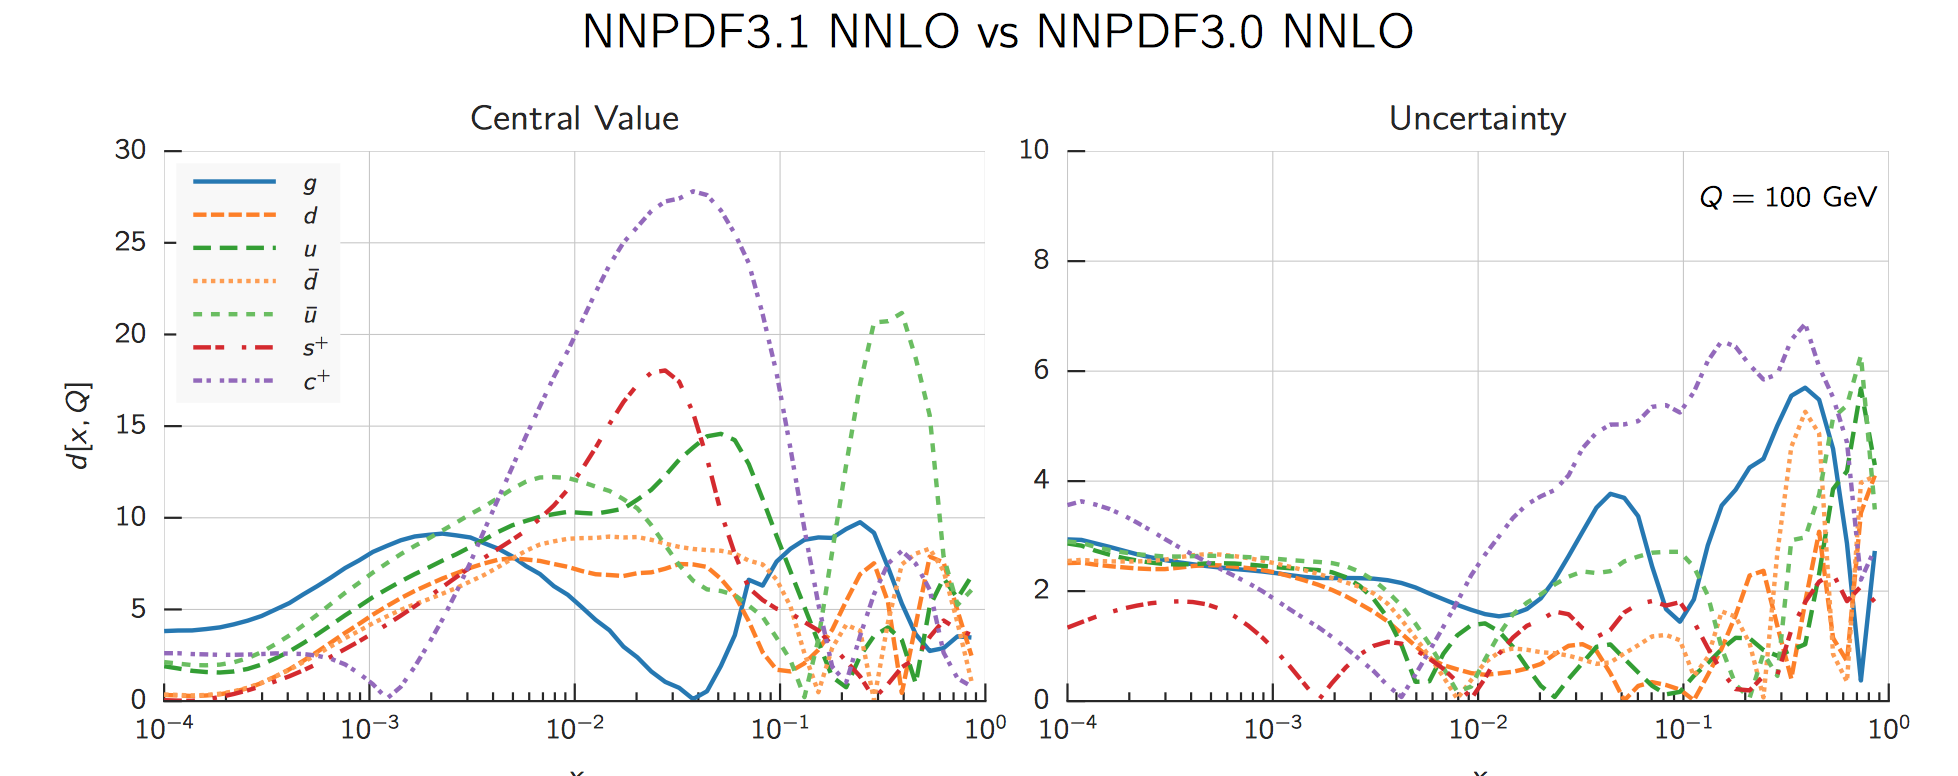
\includegraphics[width=0.1\textwidth]{Images/NNPDF_30_31}
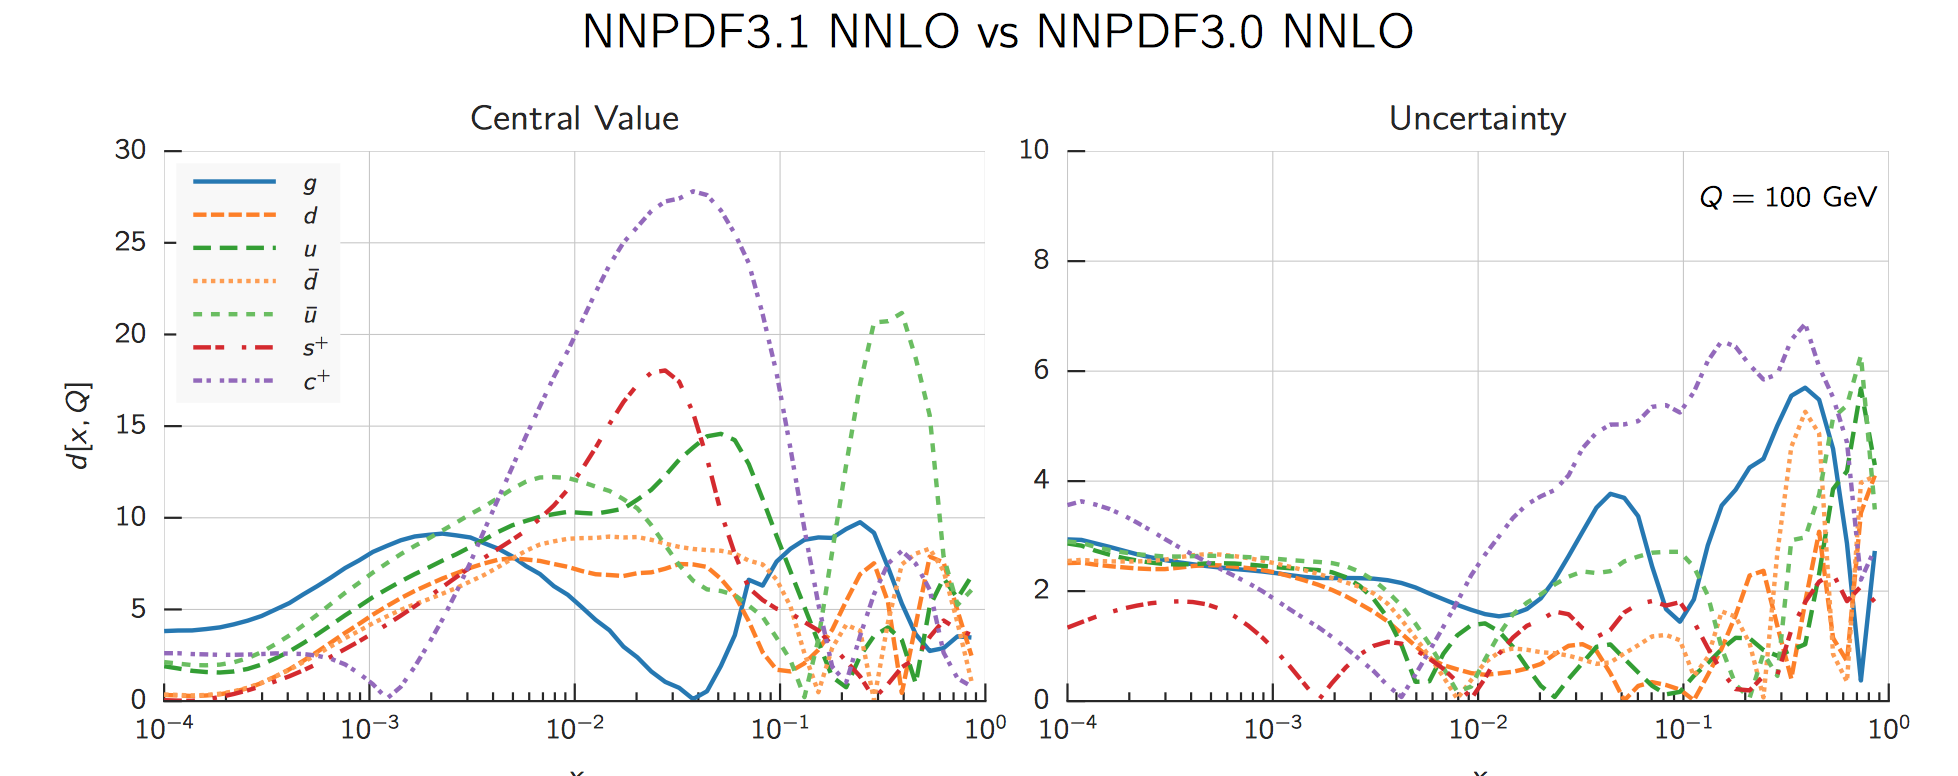
\includegraphics[width=0.1\textwidth]{Images/NNPDF_30_31}
\caption{\label{fig:IDEffNmO} The single muon efficiency for each selection as N-1 for 2016 Run for only the barrel (LHS), only the endcaps (RHS), and all $\eta$ (Bottom).}
\end{figure}

\begin{figure}[htbp]
\centering
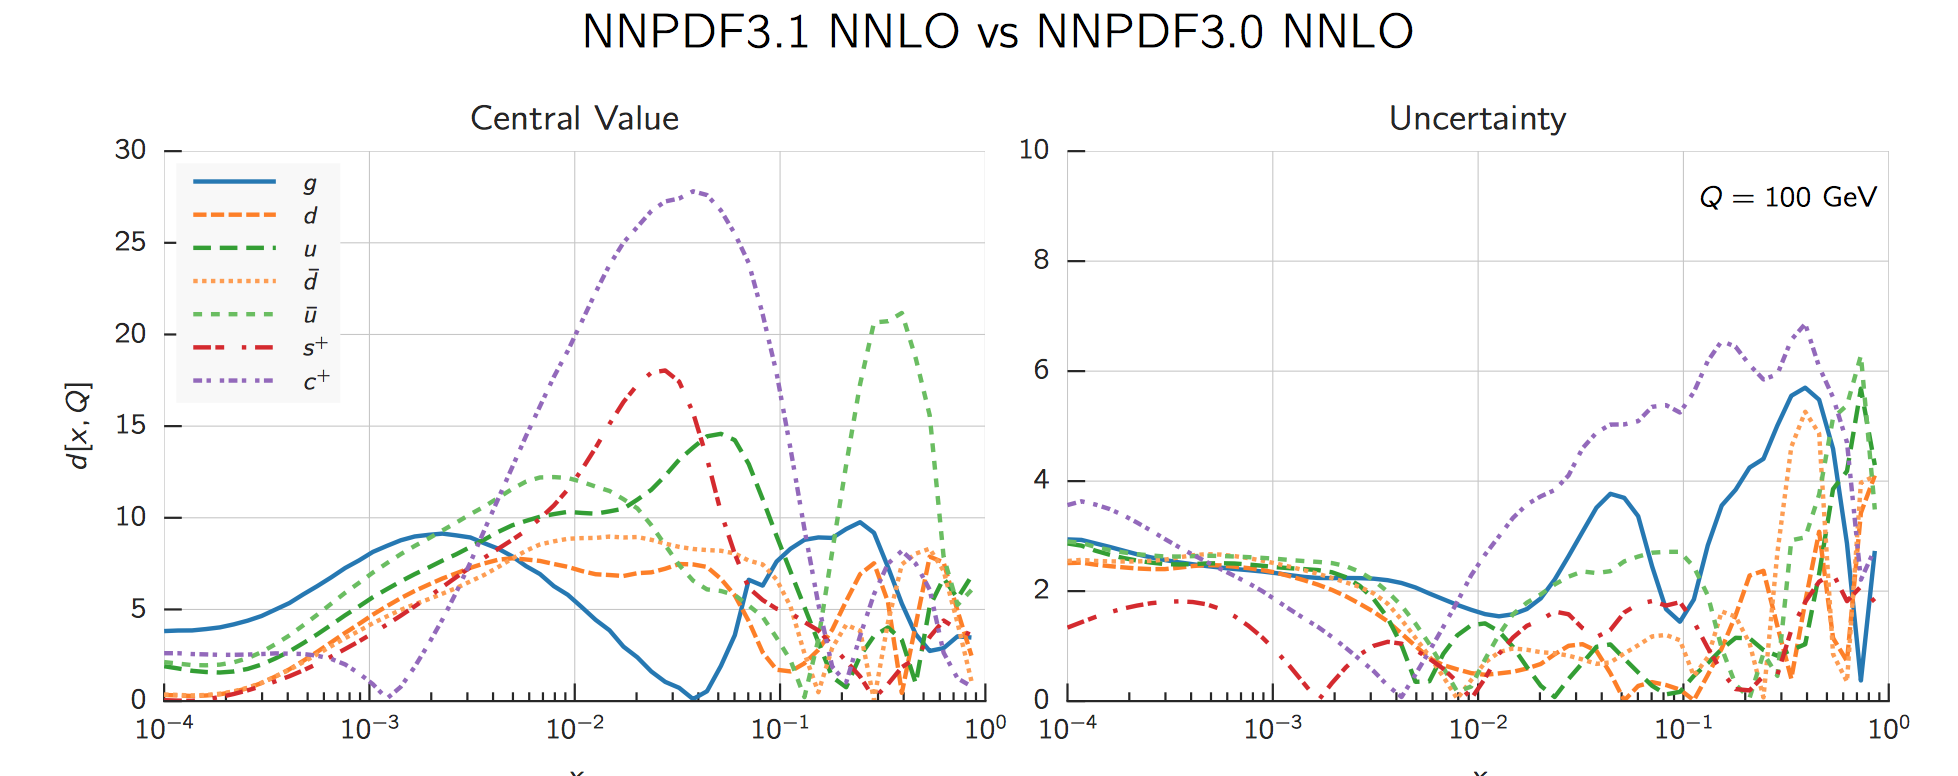
\includegraphics[width=0.1\textwidth]{Images/NNPDF_30_31}
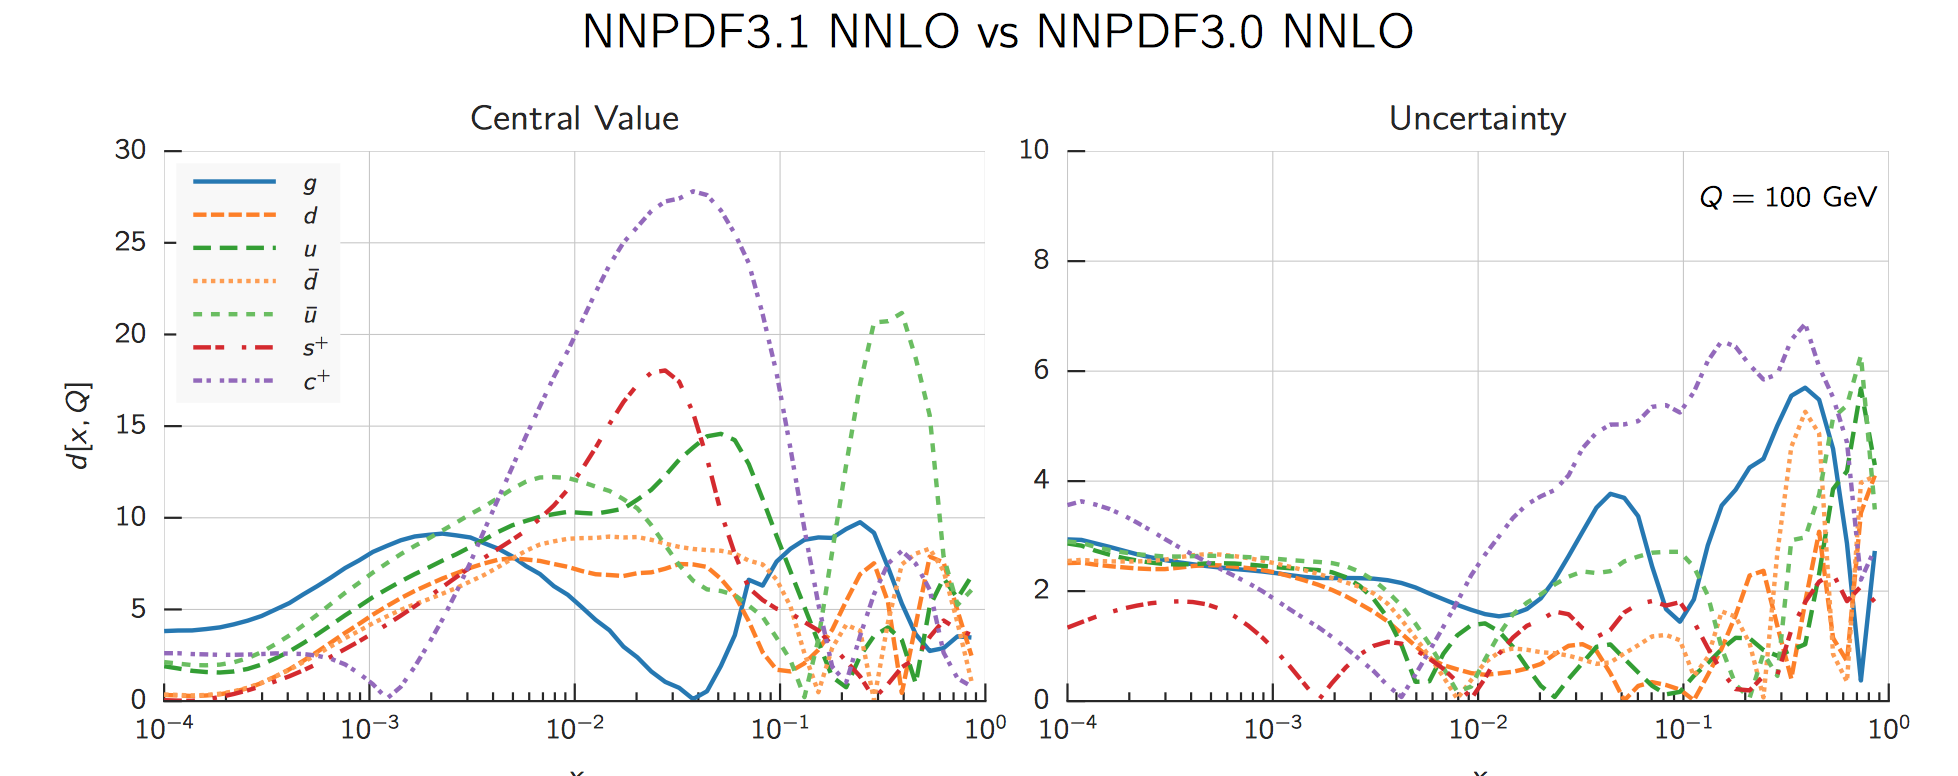
\includegraphics[width=0.1\textwidth]{Images/NNPDF_30_31}
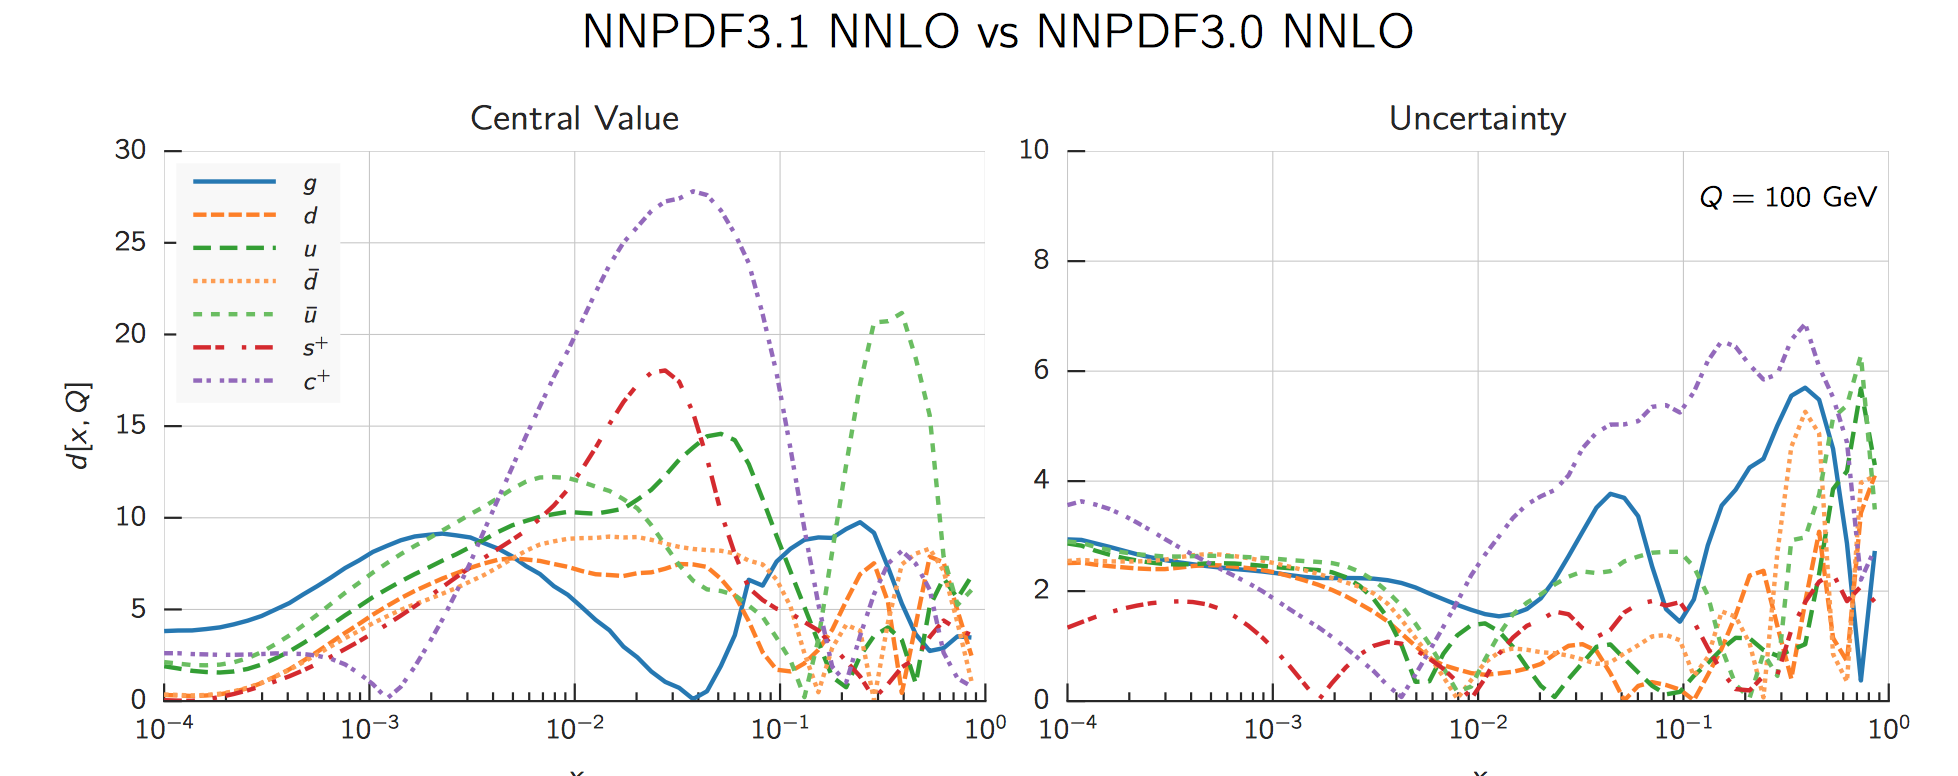
\includegraphics[width=0.1\textwidth]{Images/NNPDF_30_31}
\caption{\label{fig:IDEffNmPixHitsVsPt} The single muon efficiency for the number of pixel hits as N-1 vs muon \pt for 2016 Run for only the barrel (LHS), only the endcaps (RHS), and all $\eta$ (Bottom).}
\end{figure}

\begin{figure}[htbp]
\centering
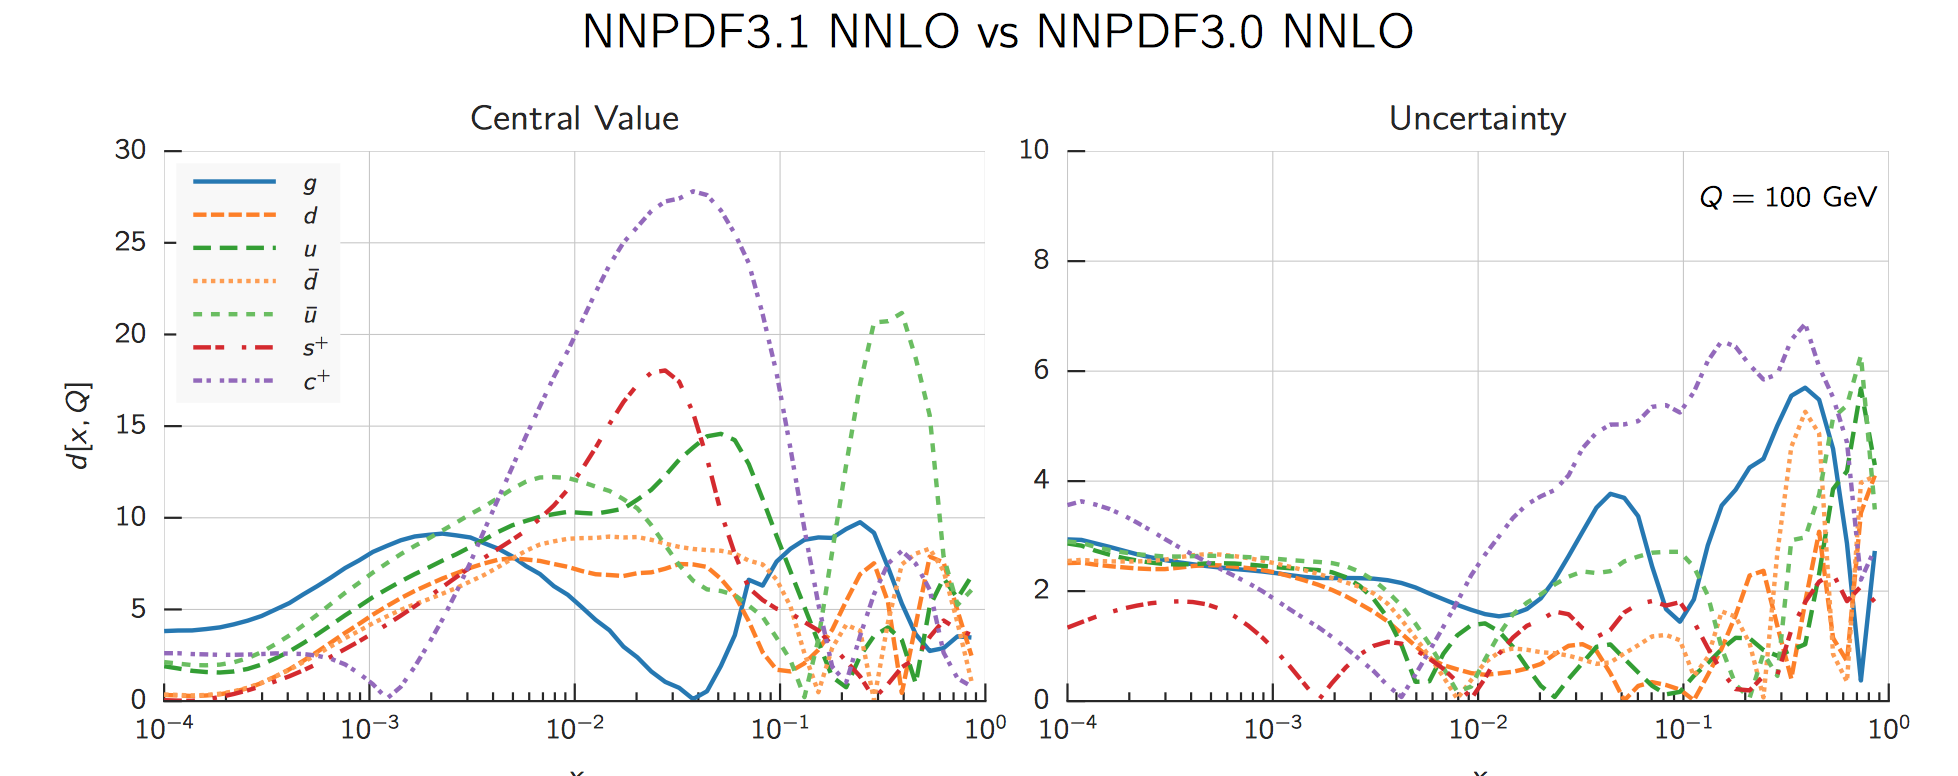
\includegraphics[width=0.1\textwidth]{Images/NNPDF_30_31}
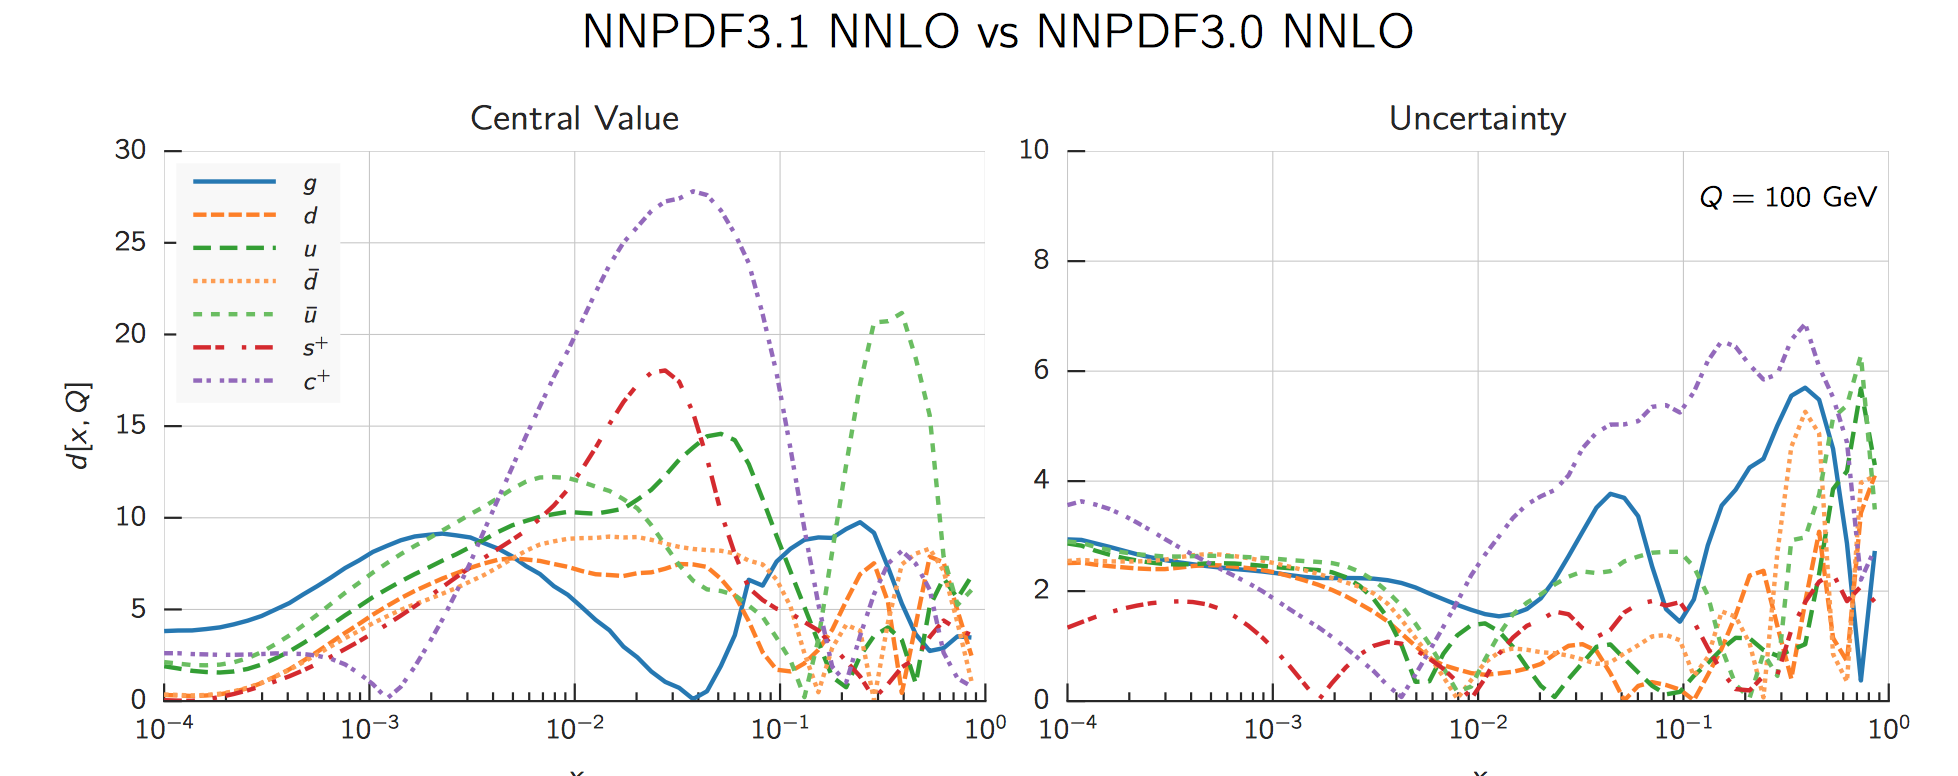
\includegraphics[width=0.1\textwidth]{Images/NNPDF_30_31}
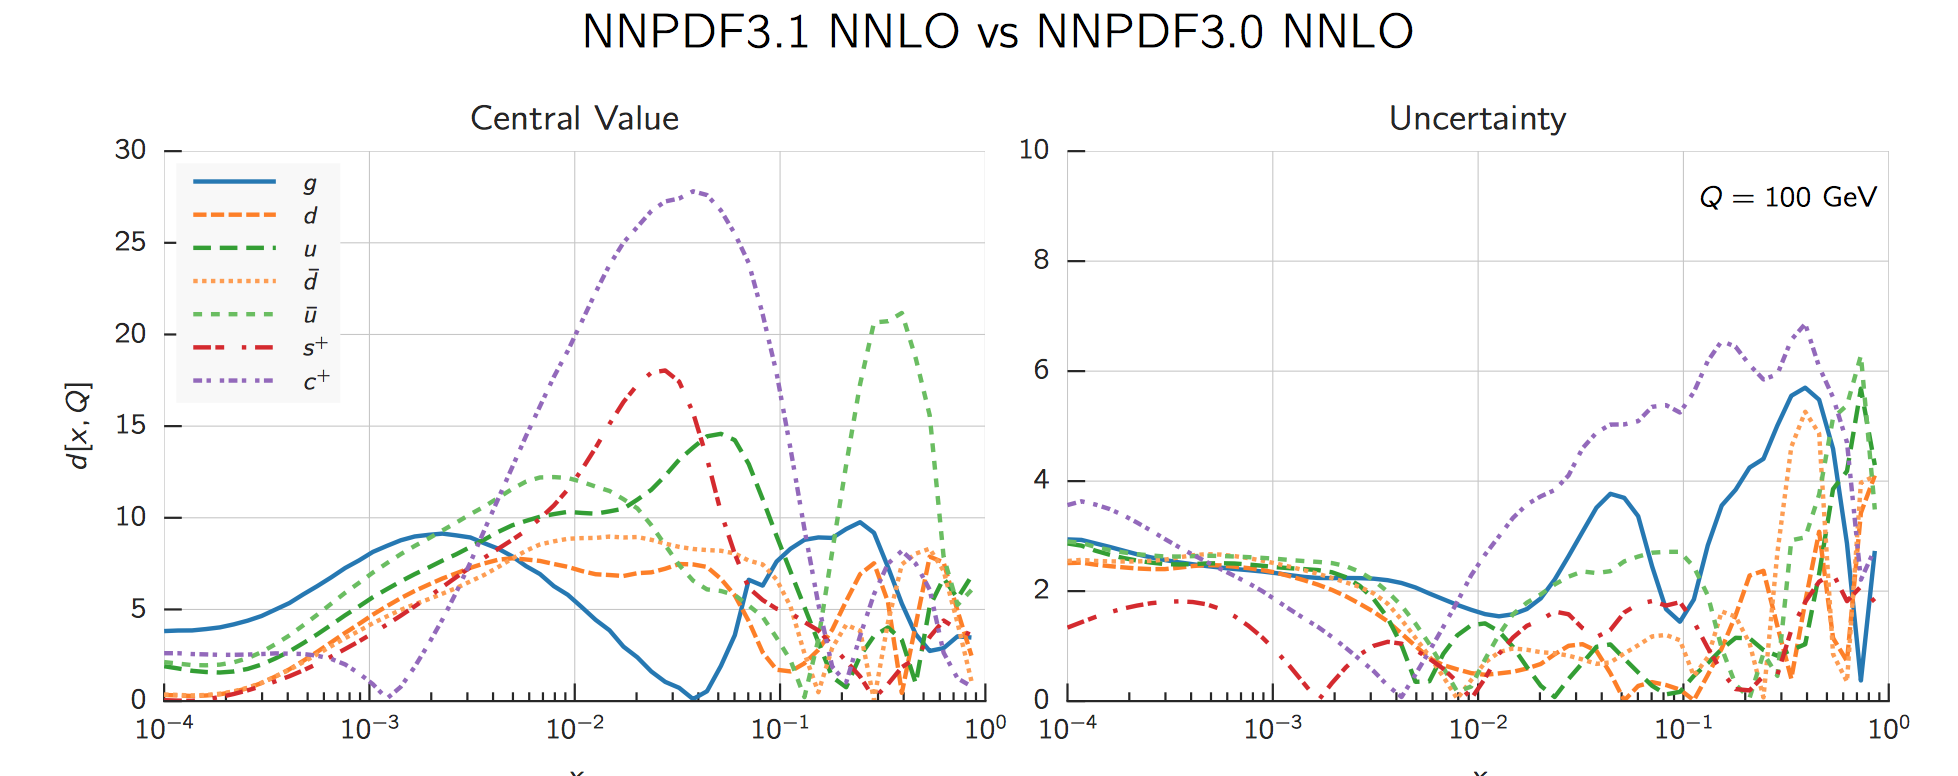
\includegraphics[width=0.1\textwidth]{Images/NNPDF_30_31}
\caption{\label{fig:IDEffNmMuoHitsVsPt} The single muon efficiency for the number of muon hits as N-1 vs muon \pt for 2016 Run for only the barrel (LHS), only the endcaps (RHS), and all $\eta$ (Bottom).}
\end{figure}
\end{comment}

\subsection{Selection efficiency}
Once the baseline selection has been set, checks on how these cuts work in data and simulations has been performed evaluating the N-1 efficiency for each cut. N-1 efficiency is calculated as the ratio of the number of events that pass all the selection cuts to the number of events passing all the cuts but the one of interest. \figurename~\ref{Nminum1} shows the 2016 N-1 efficiencies for all cuts as obtained in data and MC for two different dimuon mass ranges:
\begin{itemize}
\item 60 $< M_{\mu\mu} <$ 120GeV
\item  $M_{\mu\mu} >$ 120GeV
\end{itemize}
Same plots, done for the two $\eta$ categories (BB and BE) are reported in \figurename~\ref{Nminum1_BB} and \ref{Nminum1_BEEE}. 
The first mass range, around the Z peak, refers to a well known physics region and is used to check unexpected effects. In \figurename~\ref{Nminus1_vs_mass} the N-1 efficiency for some cuts as a function of mass is reported. \tablename~\ref{table:Nminus1_20162017} summarises the value of the N-1 efficiencies comparing with the ones evaluated in 2017, data and MC. \\
\textbf{RIFAI TUTTI I PLOT 2016 E AGGIUNGI I PLOT VS MASS A SECONDA DI QUELLI PIU DIVERSI FRA 2016 E 2017}
\begin{figure}[htbp]
\centering
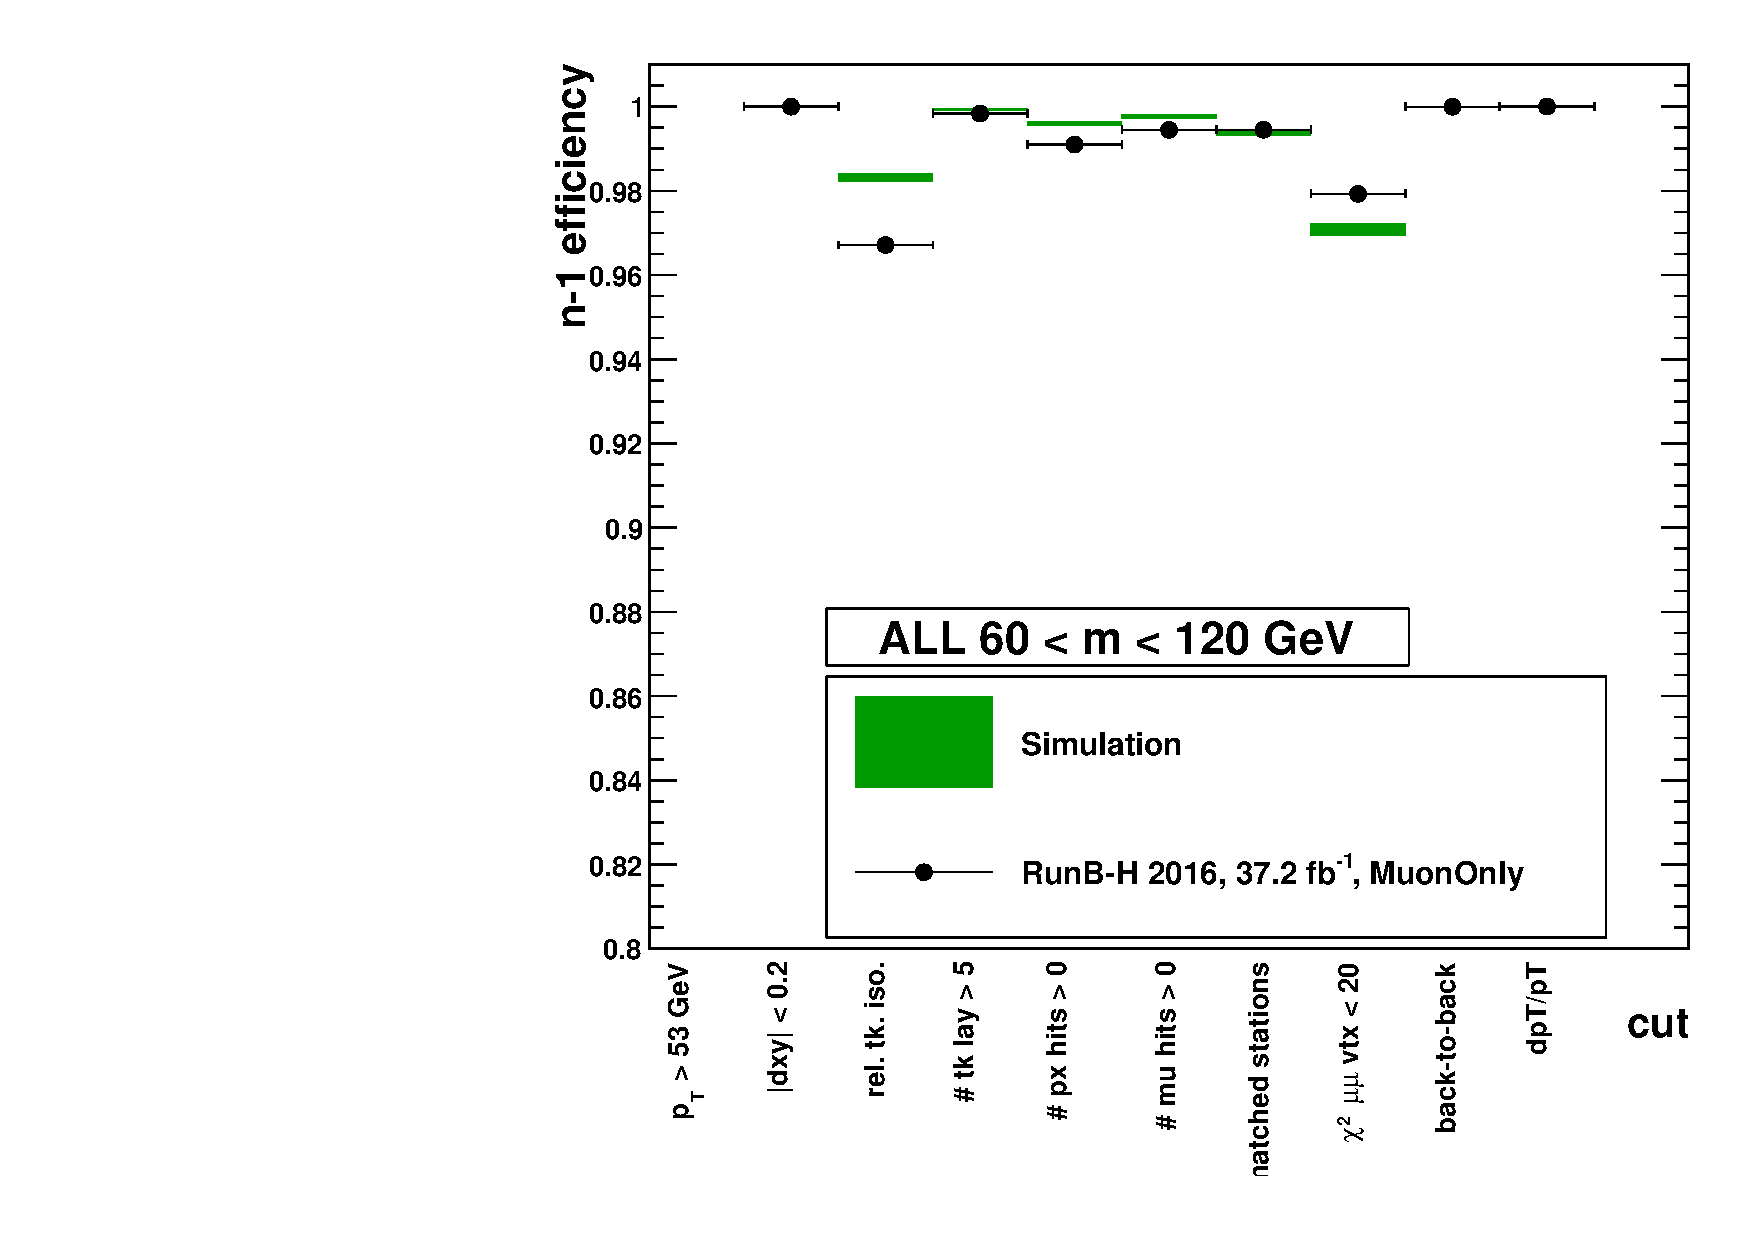
\includegraphics[width=0.4\textwidth]{Images/Cap5/60m120ALL.pdf}
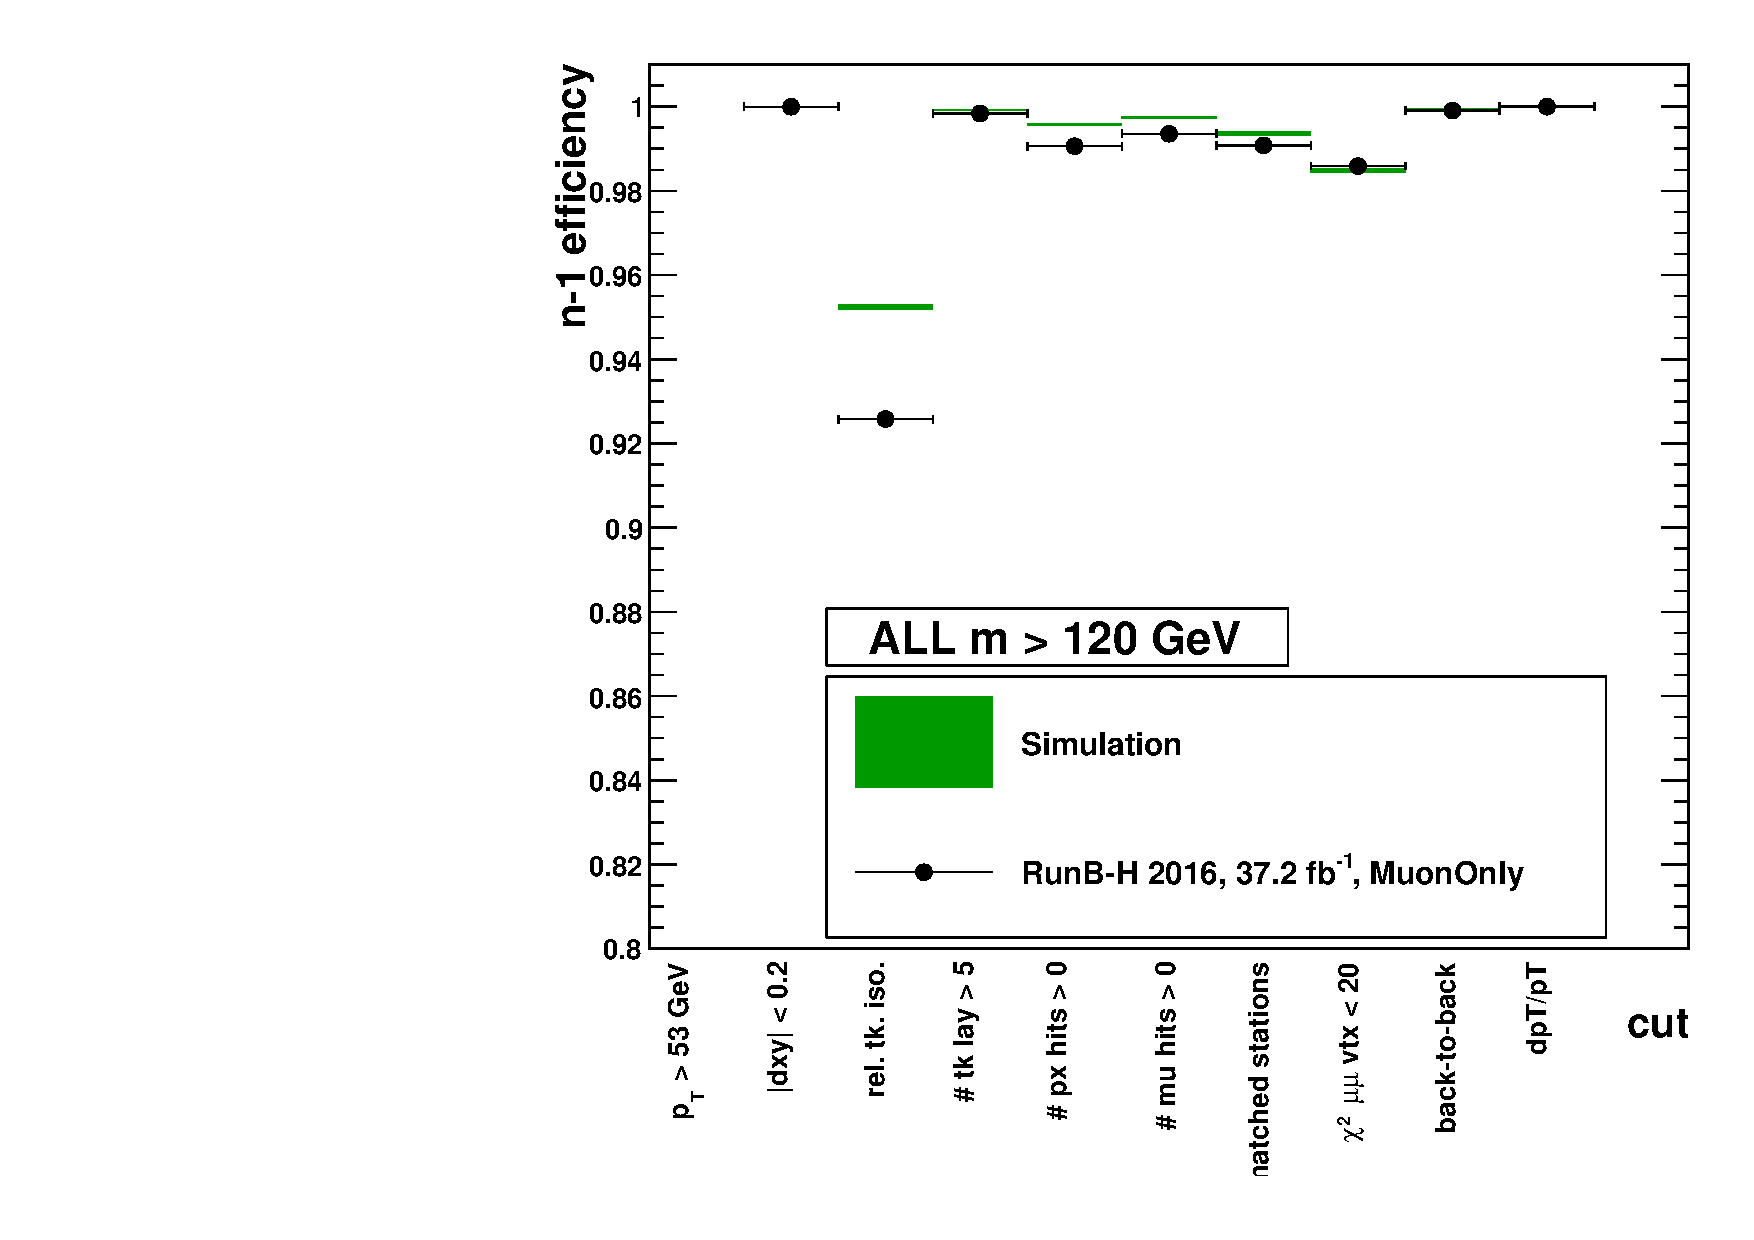
\includegraphics[width=0.4\textwidth]{Images/Cap5/120mALL.pdf}
\caption{The ratio of the number of events that pass all selection cuts to the number of events passing all cuts but the one indicated for the regions: 60 $< M_{\mu\mu} <$ 120GeV (left) and $M_{\mu\mu} >$ 120GeV (right). Here ``Simulation" includes all the backgrounds.}
\label{Nminum1}
\end{figure}

\begin{figure}[htbp]
\centering
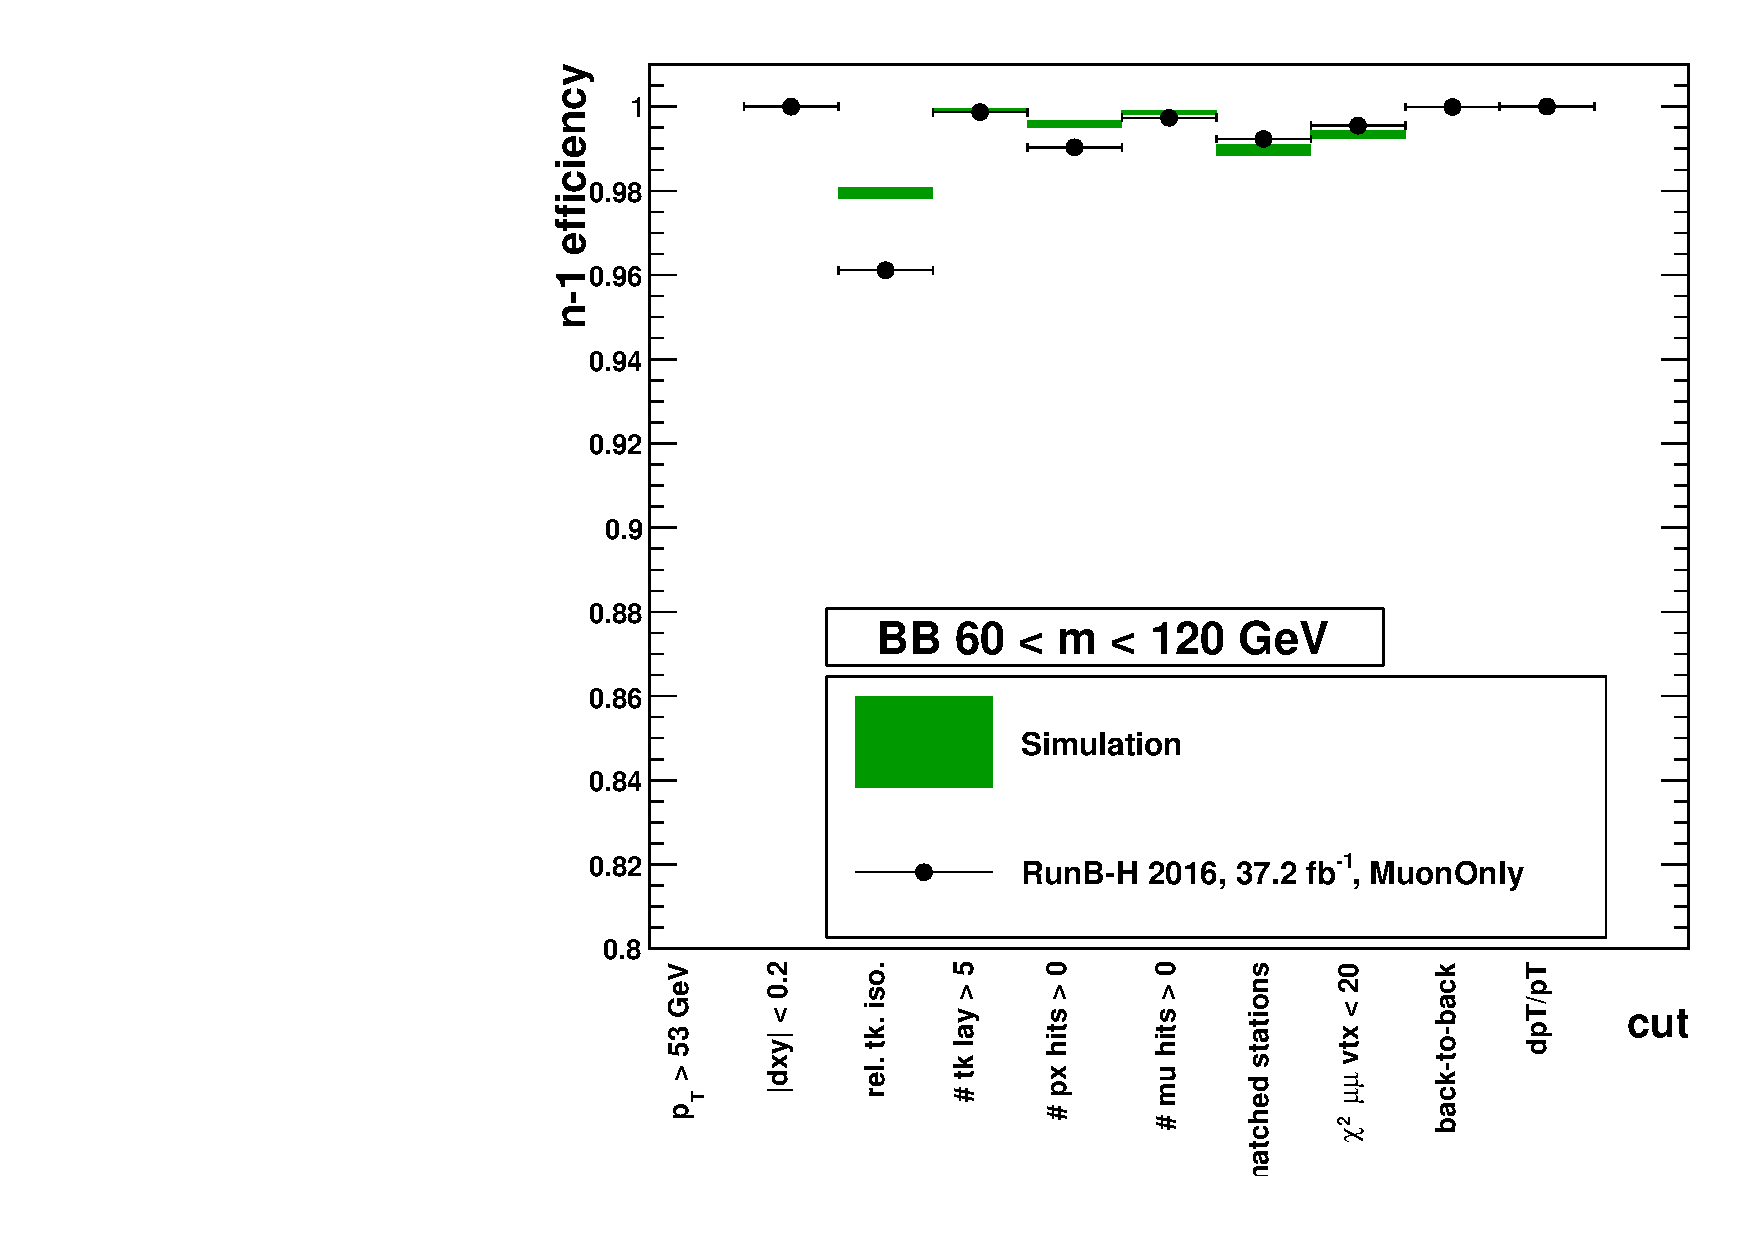
\includegraphics[width=0.4\textwidth]{Images/Cap5/60m120BB.pdf}
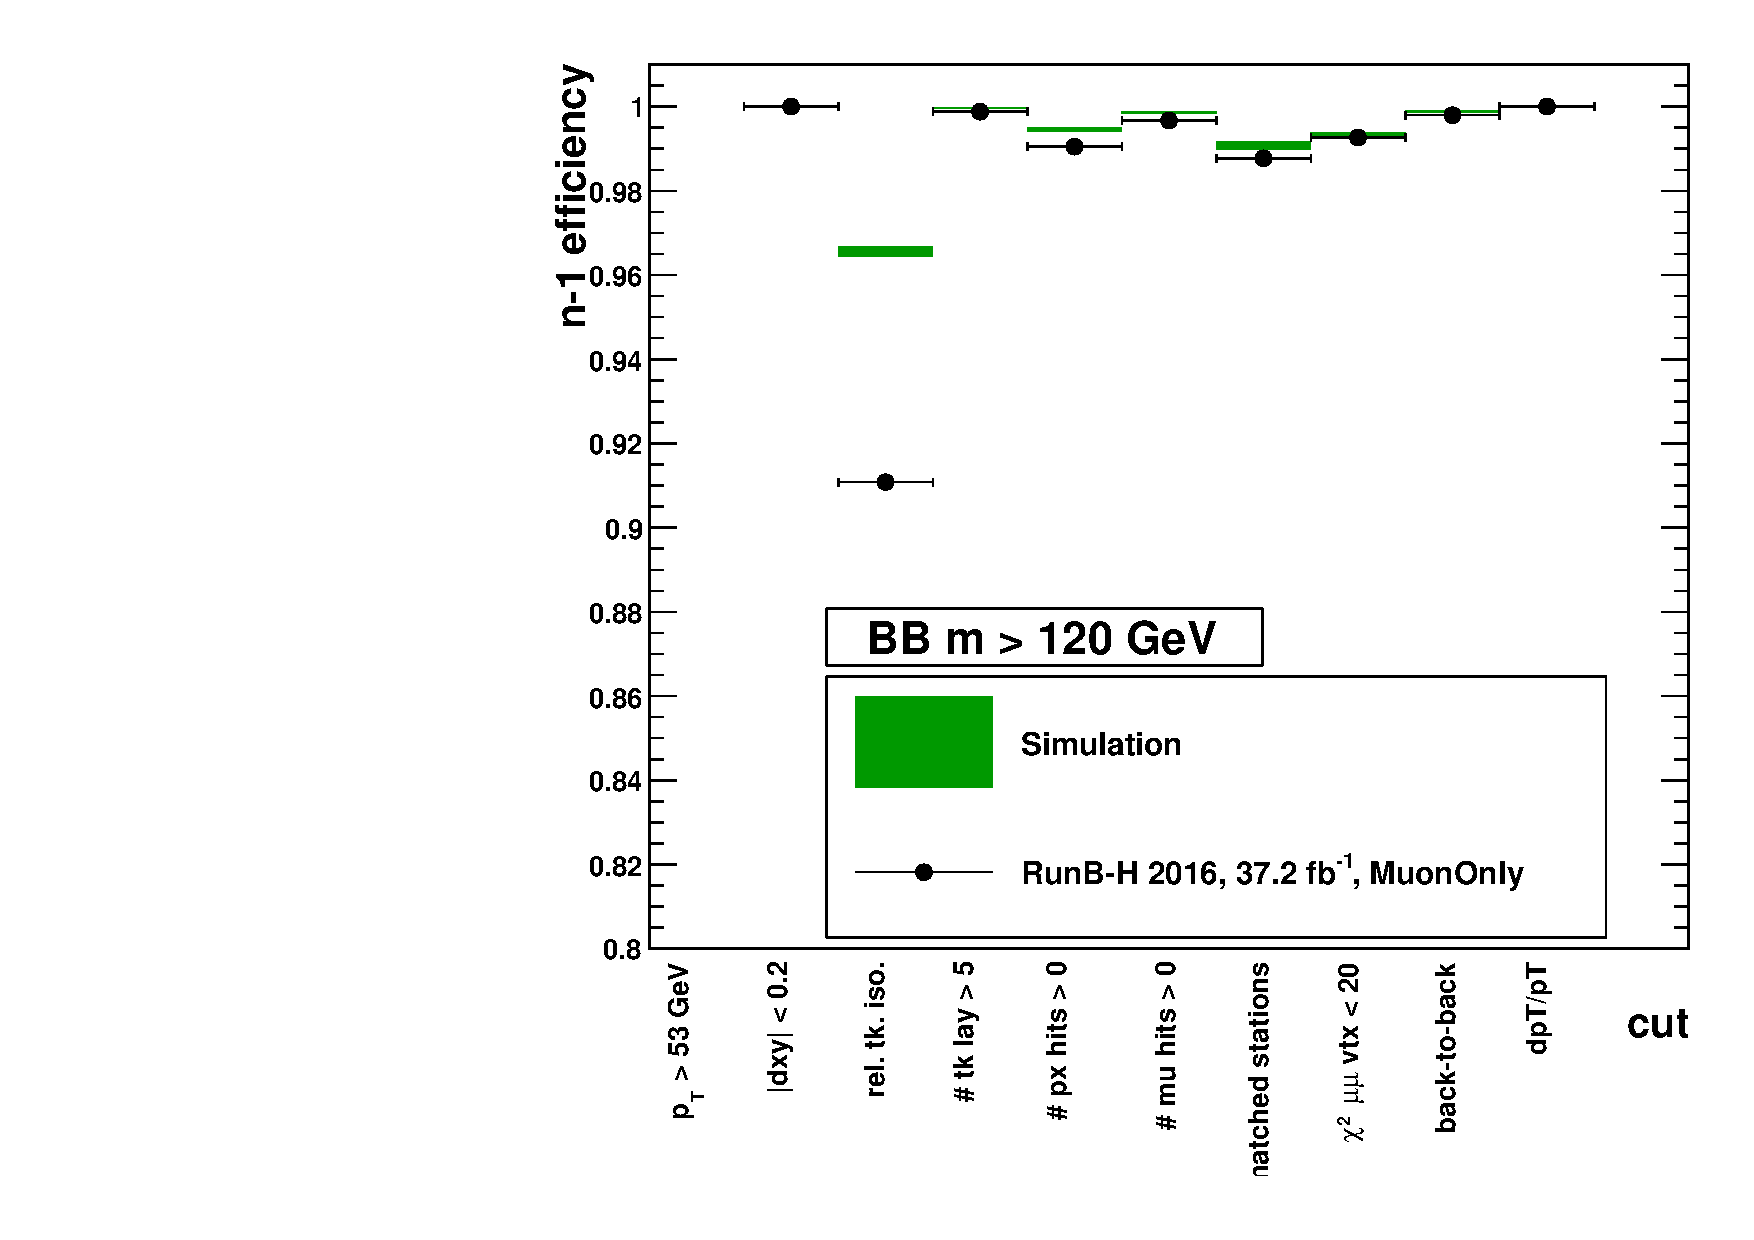
\includegraphics[width=0.4\textwidth]{Images/Cap5/120mBB.pdf}
\caption{The ratio of the number of events that pass all selection cuts to the number of events passing all cuts but the one indicated for BB category: 60 $< M_{\mu\mu} <$ 120GeV (left) and $M_{\mu\mu} >$ 120GeV (right). Here ``Simulation" includes all the backgrounds.}
\label{Nminum1_BB}
\end{figure}

\begin{figure}[htbp]
\centering
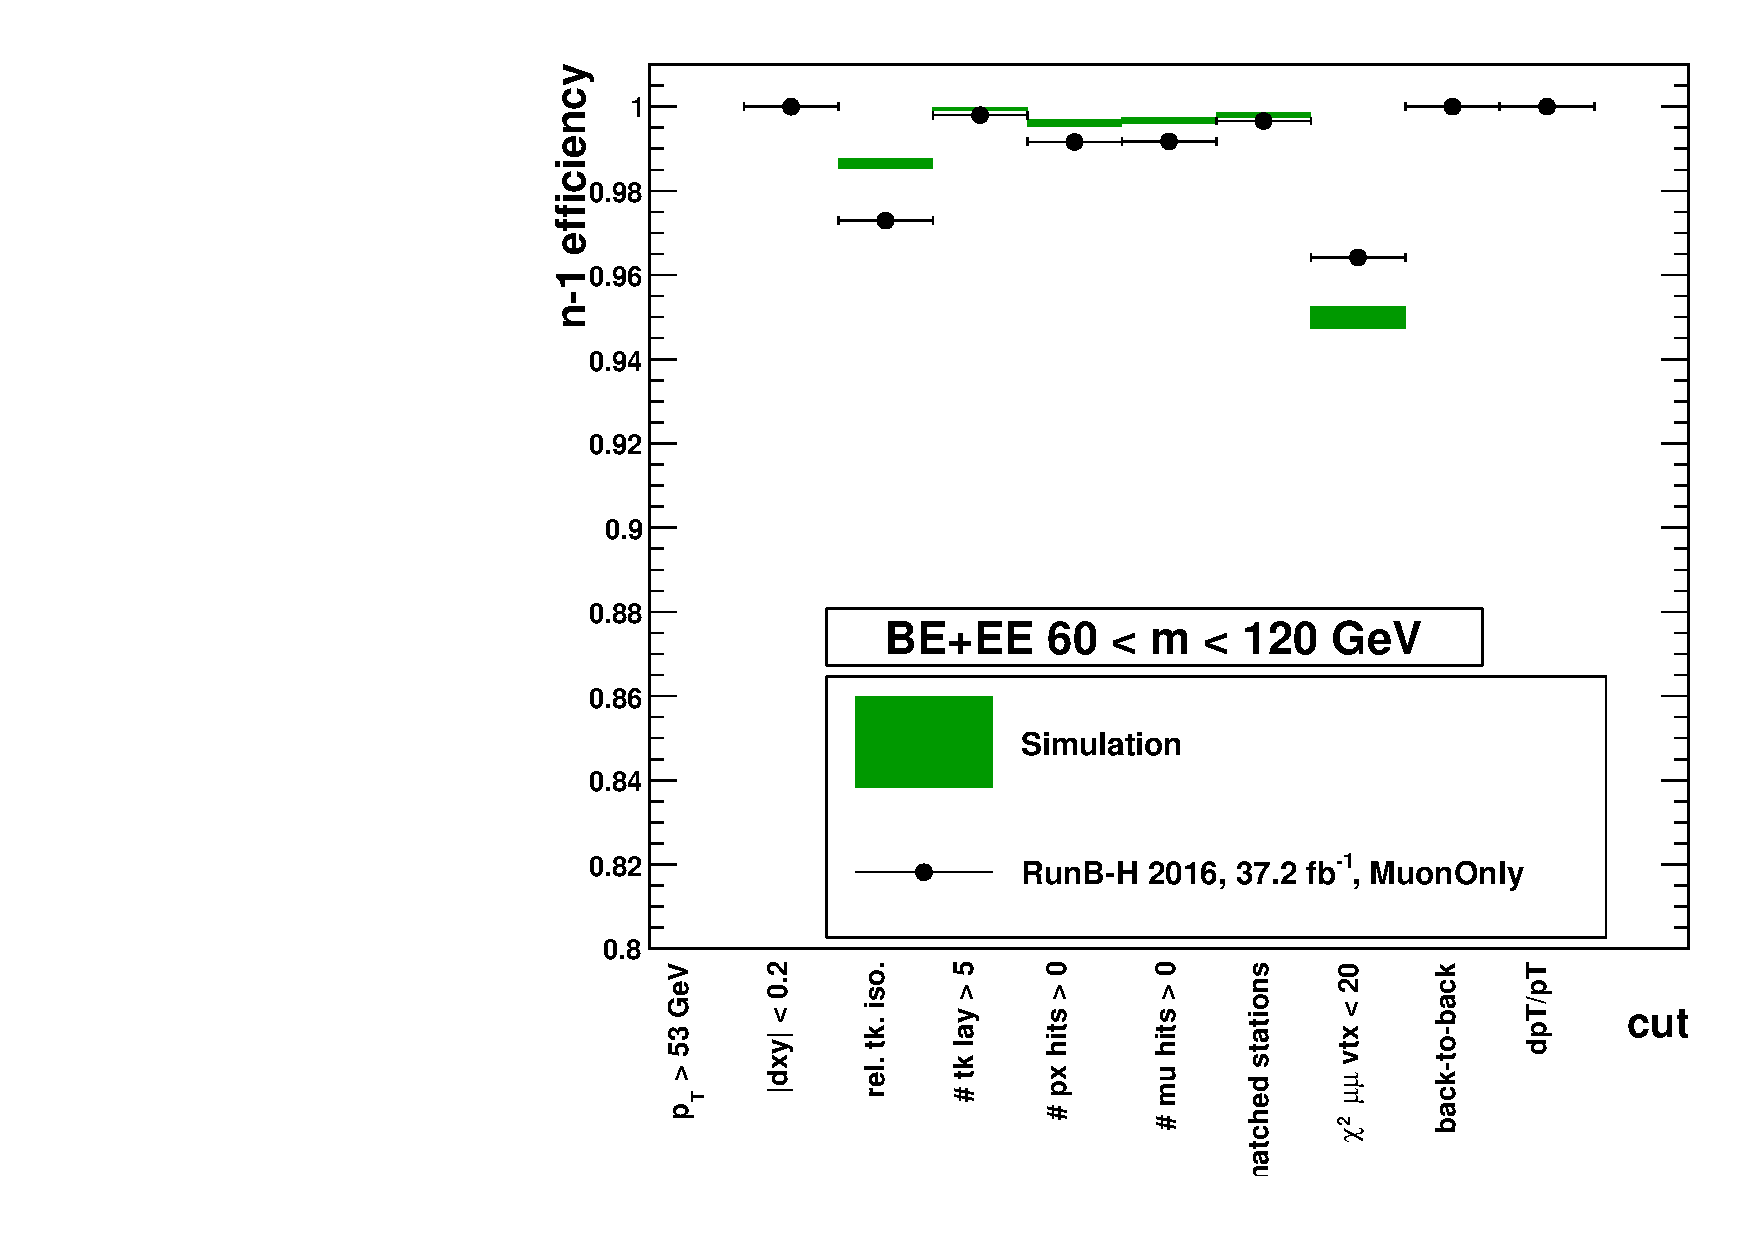
\includegraphics[width=0.4\textwidth]{Images/Cap5/60m120BE.pdf}
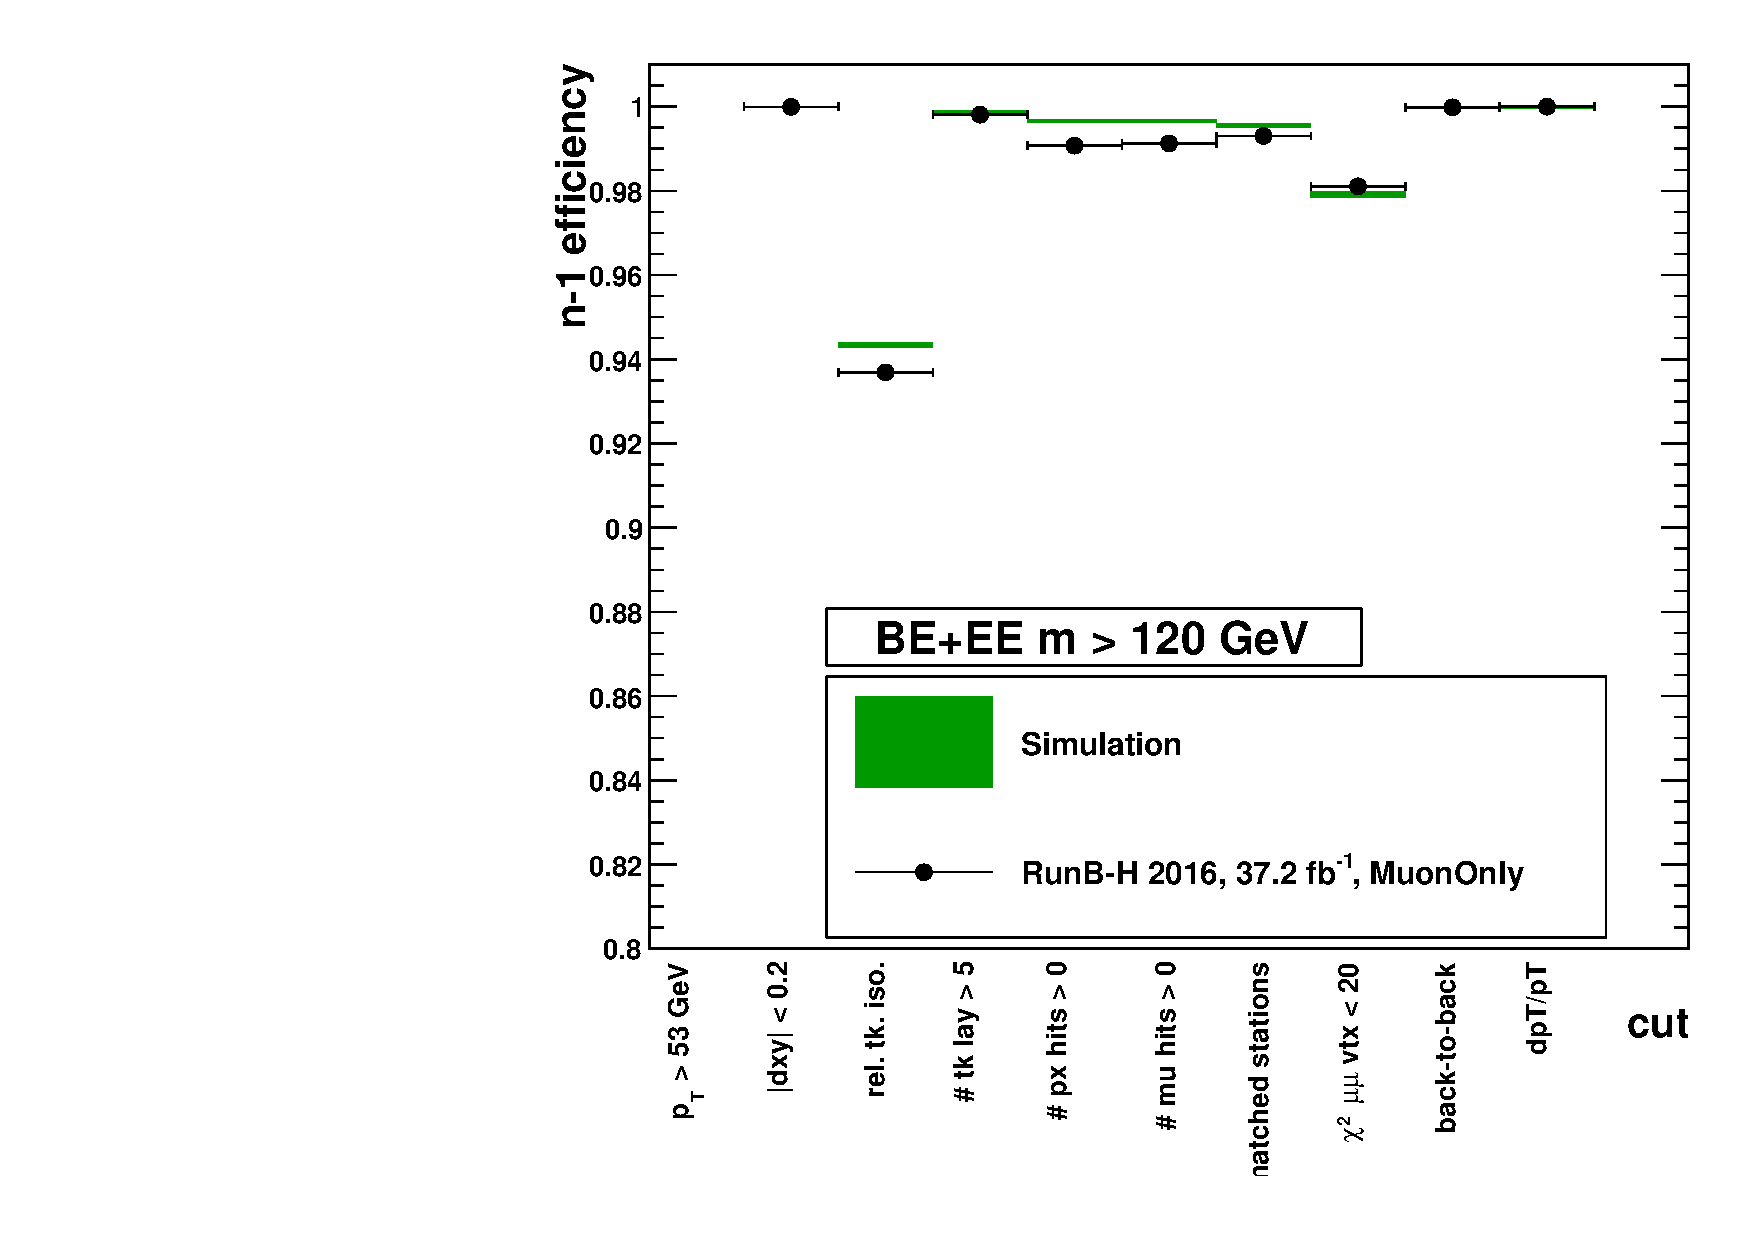
\includegraphics[width=0.4\textwidth]{Images/Cap5/120mBE.pdf}
\caption{The ratio of the number of events that pass all selection cuts to the number of events passing all cuts but the one indicated for BE + EE category: 60 $< M_{\mu\mu} <$ 120GeV (left) and $M_{\mu\mu} >$ 120GeV (right). Here ``Simulation" includes all the backgrounds.}
\label{Nminum1_BEEE}
\end{figure}

\begin{figure}[htbp]
\centering
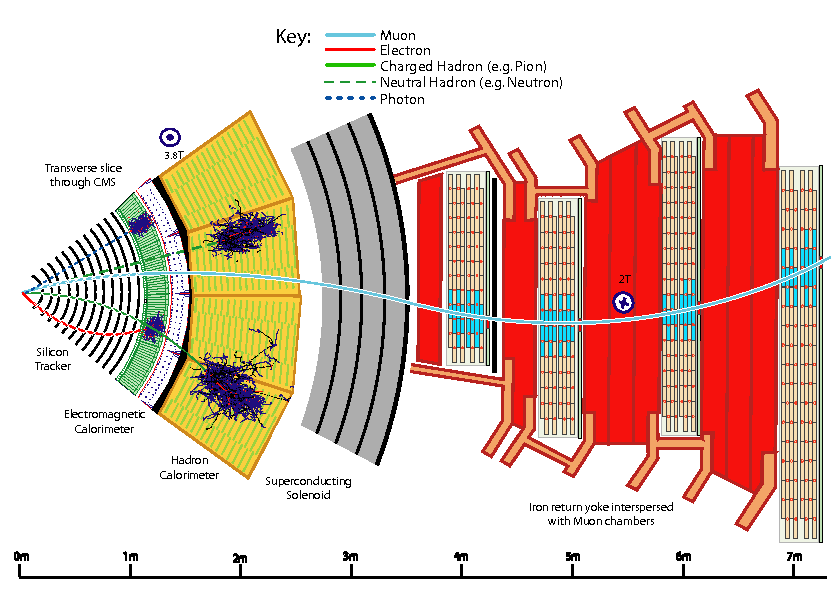
\includegraphics[width=0.1\textwidth]{Images/ParticleFlow}
\caption{vs mass}
\label{Nminus1_vs_mass}
\end{figure}

\begin{table}[htbp]
\begin{center}
\begin{tabular}{| l | l | l | l | l |}
\hline
\multirow{2}*{Cut} & \multicolumn{2}{|c|}{2016} & \multicolumn{2}{c|}{2017}\\
\cline{2-5}
 & \multicolumn{1}{|c}{MC} & DATA & MC & \multicolumn{1}{c|}{DATA}\\
\hline
\pt $>$ 53	&	0.0$\pm$ 0.0	&	0.0$\pm$ 0.0	&	0.0$\pm$ 0.0	&	0.0$\pm$ 0.0	\\
$|$dxy$|$ $<$ 0.2	&	0.0$\pm$ 0.0	&	0.0$\pm$ 0.0	&	0.0$\pm$ 0.0	&	0.0$\pm$ 0.0	\\
rel trk iso $<$ 0.1	&	0.0$\pm$ 0.0	&	0.0$\pm$ 0.0	&	0.0$\pm$ 0.0	&	0.0$\pm$ 0.0	\\
\# trk layers $>$ 5	&	0.0$\pm$ 0.0	&	0.0$\pm$ 0.0	&	0.0$\pm$ 0.0	&	0.0$\pm$ 0.0	\\
\# pixel hits $>$ 0	&	0.0$\pm$ 0.0	&	0.0$\pm$ 0.0	&	0.0$\pm$ 0.0	&	0.0$\pm$ 0.0	\\
\# mu hits $>$ 0	&	0.0$\pm$ 0.0	&	0.0$\pm$ 0.0	&	0.0$\pm$ 0.0	&	0.0$\pm$ 0.0	\\
matched stats	&	0.0$\pm$ 0.0	&	0.0$\pm$ 0.0	&	0.0$\pm$ 0.0	&	0.0$\pm$ 0.0	\\
vtx $\chi^2$ $<$ 20	&	0.0$\pm$ 0.0	&	0.0$\pm$ 0.0	&	0.0$\pm$ 0.0	&	0.0$\pm$ 0.0	\\
back-to-back	&	0.0$\pm$ 0.0	&	0.0$\pm$ 0.0	&	0.0$\pm$ 0.0	&	0.0$\pm$ 0.0	\\
$\delta$\pt / \pt $<$ 0.3	&	0.0$\pm$ 0.0	&	0.0$\pm$ 0.0	&	0.0$\pm$ 0.0	&	0.0$\pm$ 0.0	\\
trigger match	&	0.0$\pm$ 0.0	&	0.0$\pm$ 0.0	&	0.0$\pm$ 0.0	&	0.0$\pm$ 0.0	\\
\hline
\end{tabular}
\caption{N-1 efficiencies for 2016 and 2017 in DATA and simulations.}
\label{table:Nminus1_20162017}
\end{center}
\end{table}
%; small discrepancies instead are present in the vertex fit cut (\textbf{see B.3}) and in the isolation cut (\textbf{see B.2}). 
%The discrepancy between data and simulation seen in the isolation variable is due to the fact that some backgrounds are missing. For a precise study we should add all the boosted Z samples, QCD and W+jets data driven and semi-leptonic TTbar. The discrepancy observed at Z peak for the vertex cut is currently being checked but we think it is due to larger error on the track quality for lower momentum.

\begin{comment}
721 In Figure 40 and Figure 41 the N-1 efficiency for some cuts as a function of mass is reported.
722 We observed a slight deficit at high mass for the isolation variable. We know thanks to our
723 study of prompt vs Re-reco that 0.5% is due to the large numbers of spurious muons in Re-
724 reco (see Appendix A). The left over is due to the fact that we don?t have the full background
725 contribution in simulation.
726 We compare the distributions of data and simulation in order to validate that the detector be-
727 havior is understood and predictable. This is done by using the Monte Carlo simulation of
728 the background processes listed in Table 2, see Figures 42. As described earlier there are dis-
729 crepancies between data and MC for the number of hits in the silicon tracker and therefore the
730 number of tracker layers with hits.
\end{comment}

\section{Background estimation}
The main background of this analysis is related to di-muons events from DY production; at large di-muon mass the contribution from electroweak processes is not resonant but it is a continuum with a long tail. Events from \ttbar, tW, and di-bosons (WW,WZ and ZZ) provide prompt di-muons contributing over the full di-muon invariant mass spectrum. Non-prompt leptons from b-jets and mis-identified leptons can also originate in \ttbar, W+jets and multi-jets QCD events.

\subsection{Drell-Yan and Photon-induced background}
\label{sec:DYandPI}
DY samples used in this analysis are done with POWHEG at NLO in QCD and include the QED effects (like initial and final state radiation), but not the quite important at high mass pure electroweak effects and the photon induced contributions (PI). In order to convert POWHEG simulation, listed in \tablename~\ref{table:MCsamples}, to FEWZ predictions including all effects (NNLO+PI), based on the LUXqed\_plus\_PDF4LHC15 set, a mass-dependent correction must be measured. \\
The ratio of DY + PI background with \mbox{{\tt FEWZ}} to
DY background with POWHEG ($R_{\rm FEWZ\,/\,POWHEG}$) is shown in \figurename~\ref{fig:dypi}. The function extracted from the fit is the K factor dependent of mass used to correct our DY POWHEG samples. It is parametrized as
\begin{equation}
R_{\rm FEWZ\,/\,POWHEG} = a + b\cdot m  + c\cdot m^2 + d\cdot m^3
\end{equation}
with following values for the parameters:
\begin{equation*}
a = 1.067, \qquad b = -0.000112, \qquad c = 3.176\cdot 10^{-8}, \qquad d = -4.068\cdot 10^{-12}\,.
\end{equation*}

\begin{figure}[htbp]
\centering
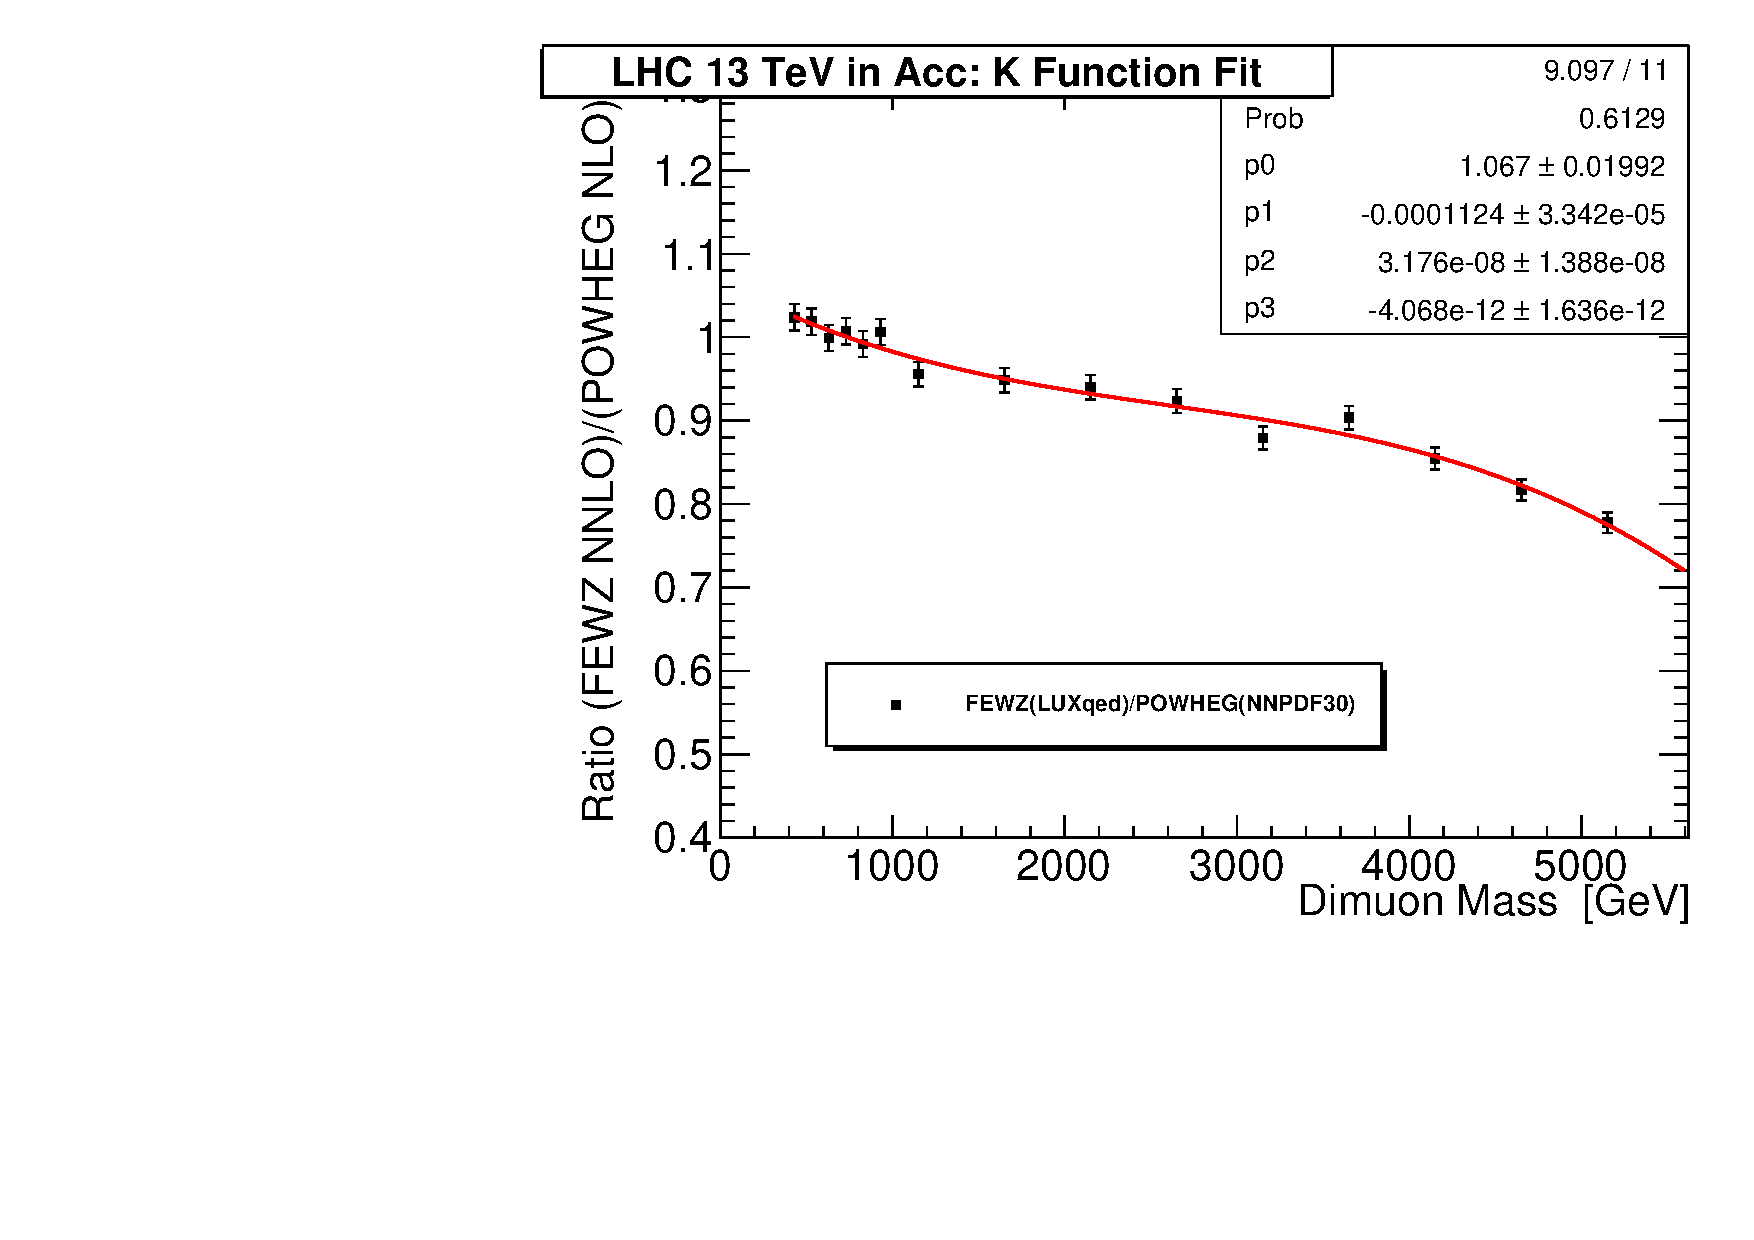
\includegraphics[width=0.5\textwidth]{Images/Cap5/lhc-mm-FEWZovPOWHEG-fit.pdf}
\caption{Ratio of di-muon cross sections computed with \mbox{{\tt FEWZ}} 
(including NNLO and PI effects) and POWHEG (as used in the analysis) with the fit function used for the K factor.}
\label{fig:dypi}
\end{figure}
\begin{comment}

For BB category the K factor used is parametrised as:
$$K_{\rm BB} = 1.036 - 0.0001441 \,X + 5.058 \cdot 10^{-8} X^2 -7.581 \cdot 10^{-12} X^3\,,$$
For BE category
$$K_{\rm BE} = 1.052 - 0.0001471 \,X + 5.903 \cdot 10^{-8} X^2 - 9.037 \cdot 10^{-12} X^3\,,$$
where $X = M-400\mbox{ GeV}$.

For $p_T>30$~GeV and $M<170$~GeV, we use for BB category
$$K_{\rm BB}^{p_T>30} = 1.003 - 0.0002904 \,X - 3.281 \cdot 10^{-6} X^2 + 5.258 \cdot 10^{-9} X^3\,,$$
for BE category
$$K_{\rm BE}^{p_T>30} = 1.012 - 0.001607 \,X + 8.796 \cdot 10^{-7} X^2 + 1.401 \cdot 10^{-6} X^3\,,$$
where $X = M-130\mbox{ GeV}$.

Figure~\ref{fig:dypi_categories} shows similar K functions computed for different $\eta$ regions and offline muon $p_T$ cuts.
\begin{figure}[!htb]
\centering
{\includegraphics[width=0.49\textwidth]{Background/figures/Dimitri_Bourilkov_apr53_FEWZovPOWHEG-fit-AL53-fine.png}}
{\includegraphics[width=0.49\textwidth]{Background/figures/Dimitri_Bourilkov_cms-mm-FEWZovPOWHEG-fit-AL30-ftwo.png}}
\\
{\includegraphics[width=0.49\textwidth]{Background/figures/Dimitri_Bourilkov_apr53_FEWZovPOWHEG-fit-BB53-fine.png}}
{\includegraphics[width=0.49\textwidth]{Background/figures/Dimitri_Bourilkov_cms-mm-FEWZovPOWHEG-fit-BB30-ftwo.png}}
\\
{\includegraphics[width=0.49\textwidth]{Background/figures/Dimitri_Bourilkov_apr53_FEWZovPOWHEG-fit-BE53-fine.png}}
{\includegraphics[width=0.49\textwidth]{Background/figures/Dimitri_Bourilkov_cms-mm-FEWZovPOWHEG-fit-BE30-ftwo.png}}
\caption{Ratio of di-muon cross sections computed with {\tt FEWZ}
(including NNLO and PI effects) and \POWHEG (as used in our simulation, see text)
with the fit function used for the K factor, 
for the whole $\eta$ region (top row),
for categories BB (middle row),
and BB+BE (bottom row).
The left plots are offline muon cut $p_T>53$~GeV,
the right ones are offline muon cut $p_T>30$~GeV (used for $Z$ normalization region).
}
\end{comment}




\subsection{TTbar estimation}
The largest background contributing to the di-muon invariant mass spectrum, following the DY production, comes from \ttbar~decays that could give two or more leptons in the final state including also two b-jets. It is possible to determine the contribution to the high \pt muon selection from \ttbar~events producing opposite-sign $\mu\mu$ events, by profiting from the fact that experimentally b-jets are tagged by using a discriminant whose value could be used to distinguish jets originating from b-jet from light-flavor quark jets. The idea is to calculate the scale factor between the data and the simulation predictions for different mass ranges, once the DY contribution is removed. The corresponding invariant mass distribution is shown in \figurename~\ref{ttbar}: the agreement between DATA and simulation is good and this proof the goodness of \ttbar~samples in representing data.

\begin{figure}[htbp]
\centering
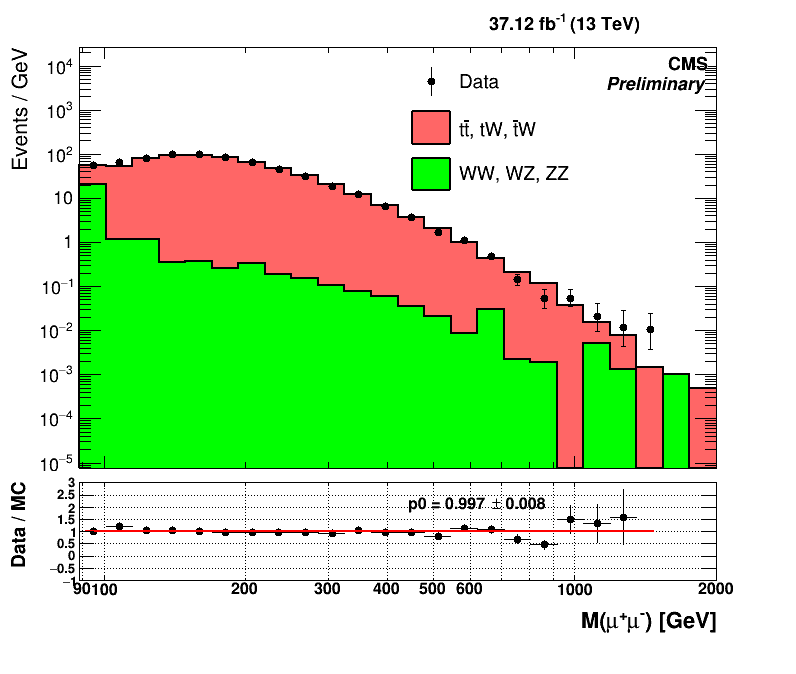
\includegraphics[width=0.4\textwidth]{Images/Cap5/TTbar-BTag-ICHEP16MCs-Data2016-mass-spectrum-MuMu-OS-37120pb_logx_after.png}
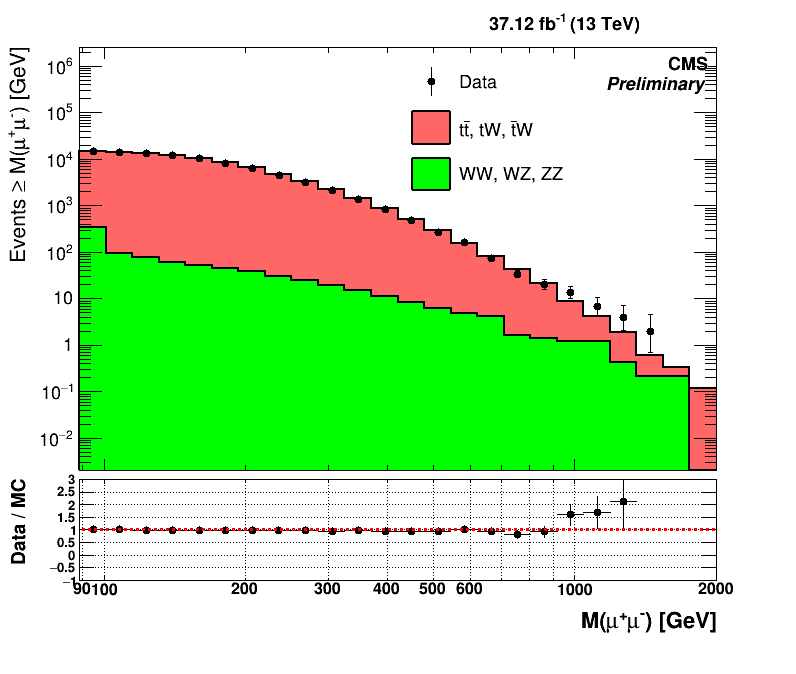
\includegraphics[width=0.4\textwidth]{Images/Cap5/TTbar-BTag-ICHEP16MCs-Data2016-cumulative-spectrum-MuMu-OS-37120pb_logx_after.png}
\caption{Observed opposite-sign dimuon invariant mass spectrum (right is cumulative one) obtained from data after subtraction of Z+jets MC. High \pt muon criteria, with 70 $<$ \Mmm $<$ 2000 GeV and in addition two b-jets are required.}
\label{ttbar}
\end{figure}

\subsection{Multijets}
Another contribution to the background in the di-muon invariant mass spectrum is due to objects mis-identified as prompt muons passing the entire selection chain, hereafter referred as ``fake" muons.
%, such as not isolated muons or hadrons mis-identified as muons. 
To estimate this contribution, a data-driven technique is used due to difficulties in simulating this process: the idea is to measure, in a control region, the ``fake rate" (FR), the probability that a fakeable object passes the high \pt muon selection used for the current analysis and then use these FR to reweight the events in order to extrapolate the contribution from ``fakes" in the signal region. The control region is defined loosing some reconstruction and/or identification criteria for the muons in order to get a phase space enriched with ``fake muons" candidates. Final contribution is determined by applying the FR measured from data to both a real data samples and simulated events selected with two muons both failing to pass the high \pt muon ID and the isolation requirements while passing the selection defining the control region. As a result, each event selected in that way is then weighted by a factor FR/(1 - FR) for each muon with a given \pt and $\eta$; so the factor is applied two times in order to estimate the
contribution of di-muons from ``fakes" (di-jets contributions). In some events, one muon passes the high-\pt muon ID and isolation requirements and a second one fail them while passing the control region selection; these events are then weighted by FR/(1 - FR) once.

\section{Yield and shape}
All the backgrounds estimated with simulation are normalized to the data in the region of the Z boson peak (60--120 GeV), and the number of expected background
events can be written as:
\begin{equation}
N^{\rm Exp} (M_{\mu\mu}\gg m_Z) = {N^{\rm Obs} (M_{\mu\mu}\gg m_Z)} \times R_Z
\label{DYexpected}
\end{equation}
where $N^{\rm Obs}_{\rm DY}$ (for $M_{\mu\mu} \gg m_Z$) is the number of background event passing the analysis selection and $R_Z$ the ratio at Z peak reported in the \tablename~\ref{tab:prescale_lumi}; for DY, the k-factor (see section \ref{sec:DYandPI}) is applied.

The number of events expected from each of the background processes, normalized to the Z peak, and the total yields from simulation, compared with data, are reported in Tables \ref{Yield}, \ref{Yield_bb} and \ref{Yield_be}. 
%To have a better view about the deficit, a fine scan of the yields as a function of mass is reported in Tables \ref{Yield_SCAN}, \ref{Yield_bb_SCAN}, \ref{Yield_be_SCAN}

\begin{table}[htb]
\begin{center}
\begin{tabular}{c|cc|ccc}
  $m_{\mu\mu}$ range & Data  & Total & Z/$\gamma^{*}$ & t$\bar{t}$ + other & Jet mis-\\
  (GeV) &      &   background   &      &  prompt bkgd    &   reconstruction\\ \hline
  120-400   &	244277	& 240326.61 &	198689.94	&	40812.27	& 824.40\\
  400-600   &	5912	& 6045.27 &	4037.73	&	1958.24	&49.30\\
  600-900   &	1311	& 1374.57 &	1002.88	&	348.29	&23.40\\
  900-1300   &	244	& 259.56 &	207.19	&	44.97	&7.40\\
  1300-1800   &	41	& 49.63 &	40.50 &	7.02	& 2.11\\
  $>$ 1800   &	8	& 12.18 &	9.37	&	1.60	&1.21\\
\end{tabular}
\caption{Numbers of events for different background processes scaled to 36.2 $fb^{-1}$ and compared to data.}
\label{Yield}
\end{center}
\end{table}

\begin{table}[htb]
\begin{center}
\begin{tabular}{c|cc|ccc}
  $m_{\mu\mu}$ range & Data  & Total & Z/$\gamma^{*}$ & t$\bar{t}$ + other & Jet mis-\\
  (GeV) &      &   background   &      &  prompt bkgd    &   reconstruction\\ \hline
  120-400   &	103644	& 100765.86 &	81075.78	&	19405.78	&284.30\\
  400-600   &	1870	&  1930.38 &	1391.67	&	526.31	&12.40\\
  600-900   &	435	& 446.06 &	358.94	&	78.52	&8.60\\
  900-1300   &	79	& 94.58 &	81.88	&	8.80	&3.90\\
  1300-1800   &	18	& 19.81 &	18.40	&	1.41	&0.0\\
  $>$ 1800   &	0	& 6.4 &	4.81	&	0.69	&0.90\\
\end{tabular}
\caption{Numbers of events for different background processes for Barrel - Barrel category scaled to 36.2 $fb^{-1}$ and compared to data.}
\label{Yield_bb}
\end{center}
\end{table}

\begin{table}[htb]
\begin{center}
\begin{tabular}{c|cc|ccc}
  $m_{\mu\mu}$ range & Data  & Total & Z/$\gamma^{*}$ & t$\bar{t}$ + other & Jet mis-\\
  (GeV) &      &   background   &      &  prompt bkgd    &   reconstruction\\ \hline
  120-400   &	140633	& 139386.57 &	117388.21	&	21458.26	&540.10\\
  400-600   &	4042	& 4097.66 &	2636.59	&	1424.17	&36.90\\ 
  600-900   &	876	& 924.80 &	642.00	&	268.00	&14.80\\
  900-1300   &	165	& 164.56 &	125.15	&	35.91	&3.50\\
  1300-1800   &	23	& 29.84 &	22.15	&	5.58& 2.11\\
  $>$ 1800   &	8	& 5.82&	4.60	&	0.91	&0.31\\
\end{tabular}
\caption{Numbers of events for different background processes for Endcap - Barrel and Endcap - Endcap category scaled to 36.2 $fb^{-1}$ and compared to data.}
\label{Yield_be}
\end{center}
\end{table}

\begin{comment}
\begin{table}[htb]
\begin{center}
\begin{tabular}{c|cc|ccc}
  $m_{\mu\mu}$ range & Data  & Total & Z/$\gamma^{*}$ & t$\bar{t}$ + other & Jet mis-\\
  (GeV) &      &   background   &      &  prompt bkgd    &   reconstruction\\ \hline
  1300-1400   &  18    &  18.36 &	15.16	&	2.60	& 0.60\\
  1400-1500   &   10   & 12.06	&	10.11	&	1.58	& 0.37\\
  1500-1600  &		8	& 8.31	& 7.00		&	0.71	& 0.60\\
  1600-1700   &    5   & 5.33	& 4.78	& 0.31	& 0.24\\
  1700-1800   &   0   & 5.55 &	3.44	&	1.81	& 0.30\\
\end{tabular}
\caption{Numbers of events for different background processes, in 1300 - 1800 GeV, range scaled to 36.2 $fb^{-1}$ and compared to data.}
\label{Yield_SCAN}
\end{center}
\end{table}

\begin{table}[htb]
\begin{center}
\begin{tabular}{c|cc|ccc}
  $m_{\mu\mu}$ range & Data  & Total & Z/$\gamma^{*}$ & t$\bar{t}$ + other & Jet mis-\\
  (GeV) &      &   background   &      &  prompt bkgd    &   reconstruction\\ \hline
  1300-1400   &      6	& 7.78  &	6.92	&	0.86	& 0.0\\
  1400-1500   &      7	& 4.75 &	4.41	&	0.34	& 0.0\\
  1500-1600  &       3	& 3.28	&	3.18	&	0.10	& 0.0\\
  1600-1700   &	2	 & 2.30 	&	2.24	&	0.06	& 0.0\\
  1700-1800   &      0	& 1.73 &	1.69	&	0.04	& 0.0\\
\end{tabular}
\caption{Numbers of events for different background processes for Barrel - Barrel category, in 1300 - 1800 GeV range, scaled to 36.2 $fb^{-1}$ and compared to data.}
\label{Yield_bb_SCAN}
\end{center}
\end{table}

\begin{table}[htb]
\begin{center}
\begin{tabular}{c|cc|ccc}
  $m_{\mu\mu}$ range & Data  & Total & Z/$\gamma^{*}$ & t$\bar{t}$ + other & Jet mis-\\
  (GeV) &      &   background   &      &  prompt bkgd    &   reconstruction\\ \hline
  1300-1400   &	12      & 10.59 & 8.26		&	1.73	& 0.60\\
  1400-1500   &	3      & 7.31 	&	5.70	&	1.24	& 0.37\\
  1500-1600  &     5  & 5.05	&	3.84	&	0.61	& 0.60\\
  1600-1700   &	3       & 3.05 &	2.56	&	0.25	& 0.24\\
  1700-1800   &	0      & 3.85	&	1.80	&	1.75	& 0.30\\
\end{tabular}
\caption{Numbers of events for different background processes for Endcap - Barrel and Endcap - Endcap category, in 1300 -1800 GeV range, scaled to 36.2 $fb^{-1}$ and compared to data.}
\label{Yield_be_SCAN}
\end{center}
\end{table}
\end{comment}

\subsubsection{Background shape} 
The background shape is obtained adding all the backgrounds; its parametrization is determined by the fit to the simulated  dimuon mass spectrum using the following function \ref{eqn:bkgshape}.

\begin{equation}
\begin{small}
f_{bkg}(m\mid a_{L}, b_{L}, c_{L}, k_{L}, a_{H}, b_{H}, c_{H}, d_{H}, k_{H}) = \begin{cases}
e^{a_{L} + b_{L}\times m + c_{L}\times m^2}m^{k_{L}}, & \mbox{if }m \le \mbox{500 GeV} \\
e^{a_{H} + b_{H}\times m + c_{H}\times m^2 + d_{H}\times m^3}m^{k_{H}}, & \mbox{if }m > \mbox{500 GeV} \end{cases}
\end{small}
\label{eqn:bkgshape}
\end{equation}

The fit is performed in the mass range 150-5000 GeV for every
pseudo-rapidity category.
Splitting function in two mass ranges, let to better fit the tail of the distribution,
with a good agreement also in the low mass region.
In \figurename~\ref{fig:bkg_fit} are shown the fits of the background shape while
in \figurename~\ref{fig:bkg_res} are shown the residuals for both the categories.
\begin{figure}[htbp]
\centering
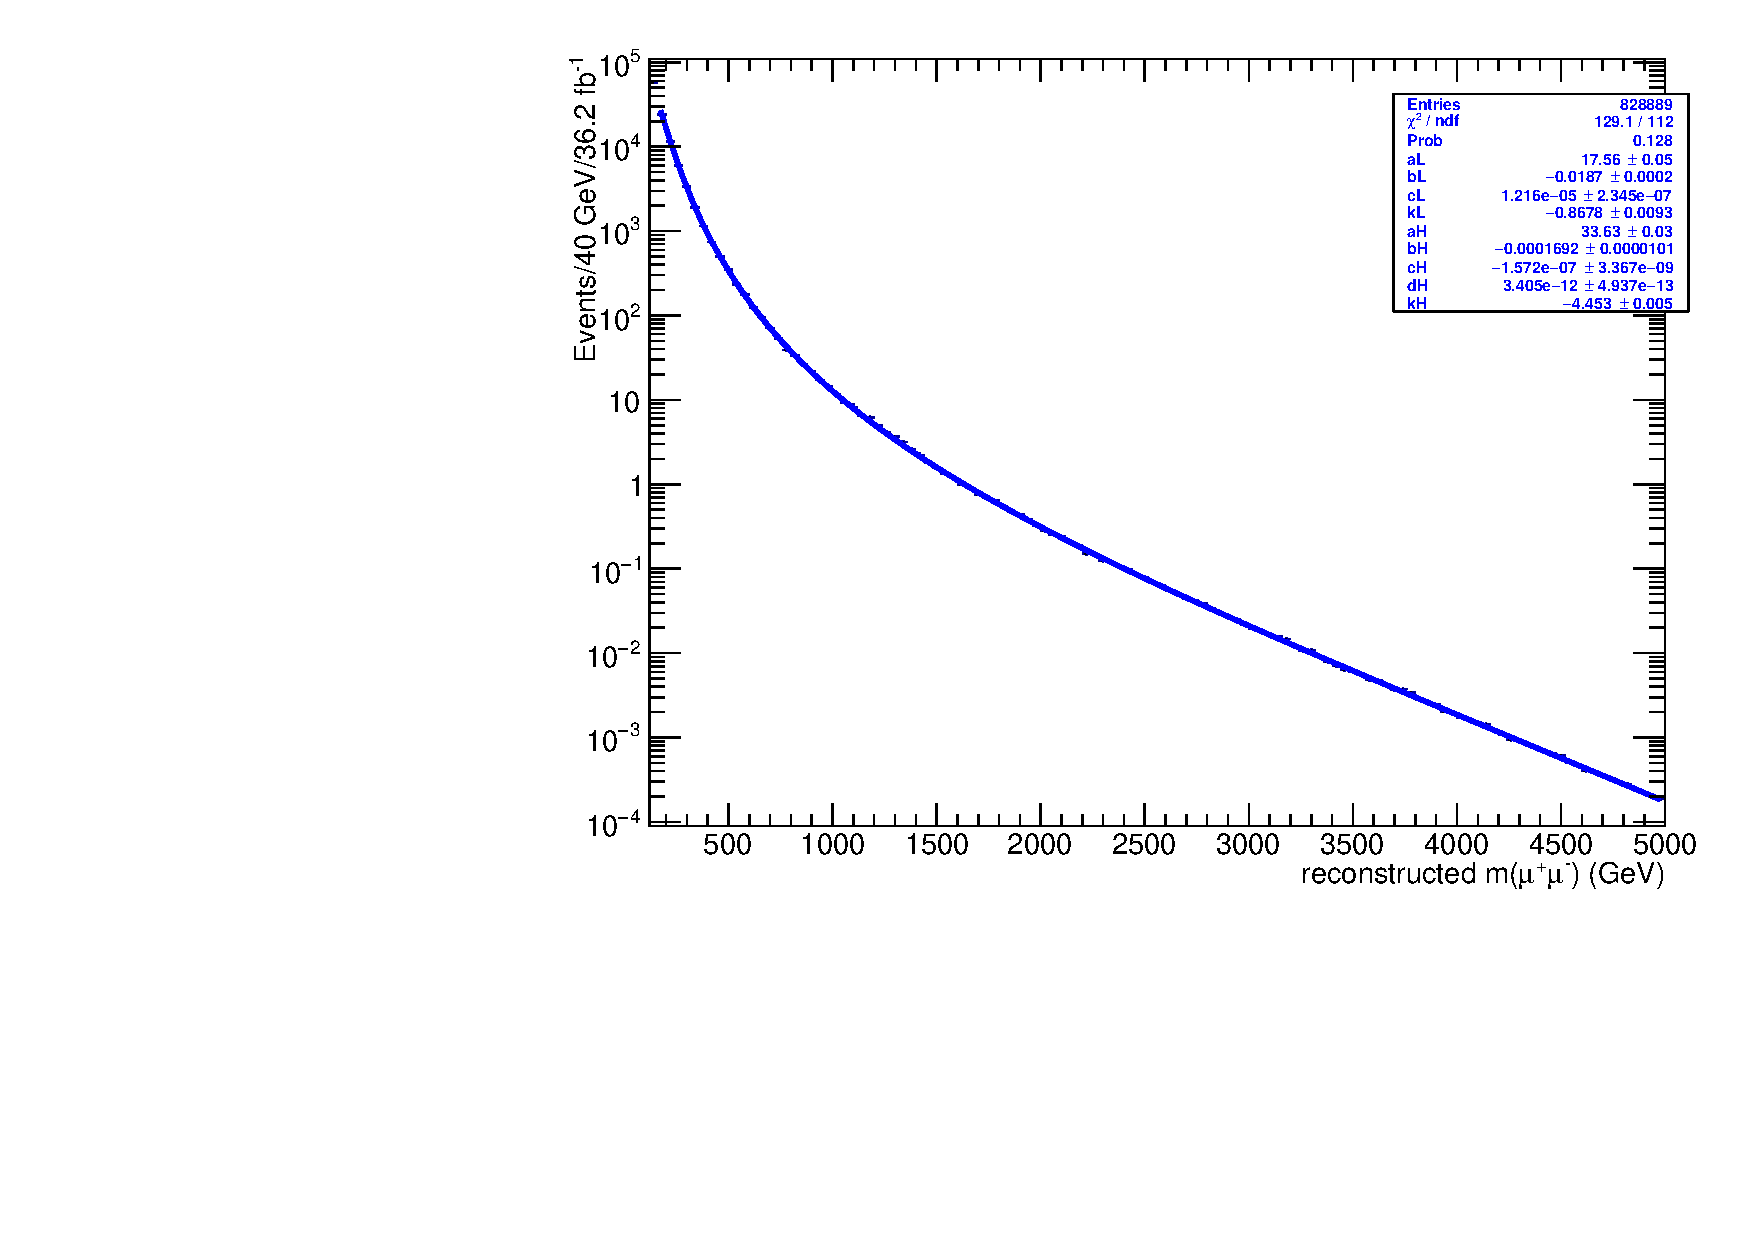
\includegraphics[width=0.47\textwidth]{Images/Cap5/mass150_5000_log_BB_9par.pdf}
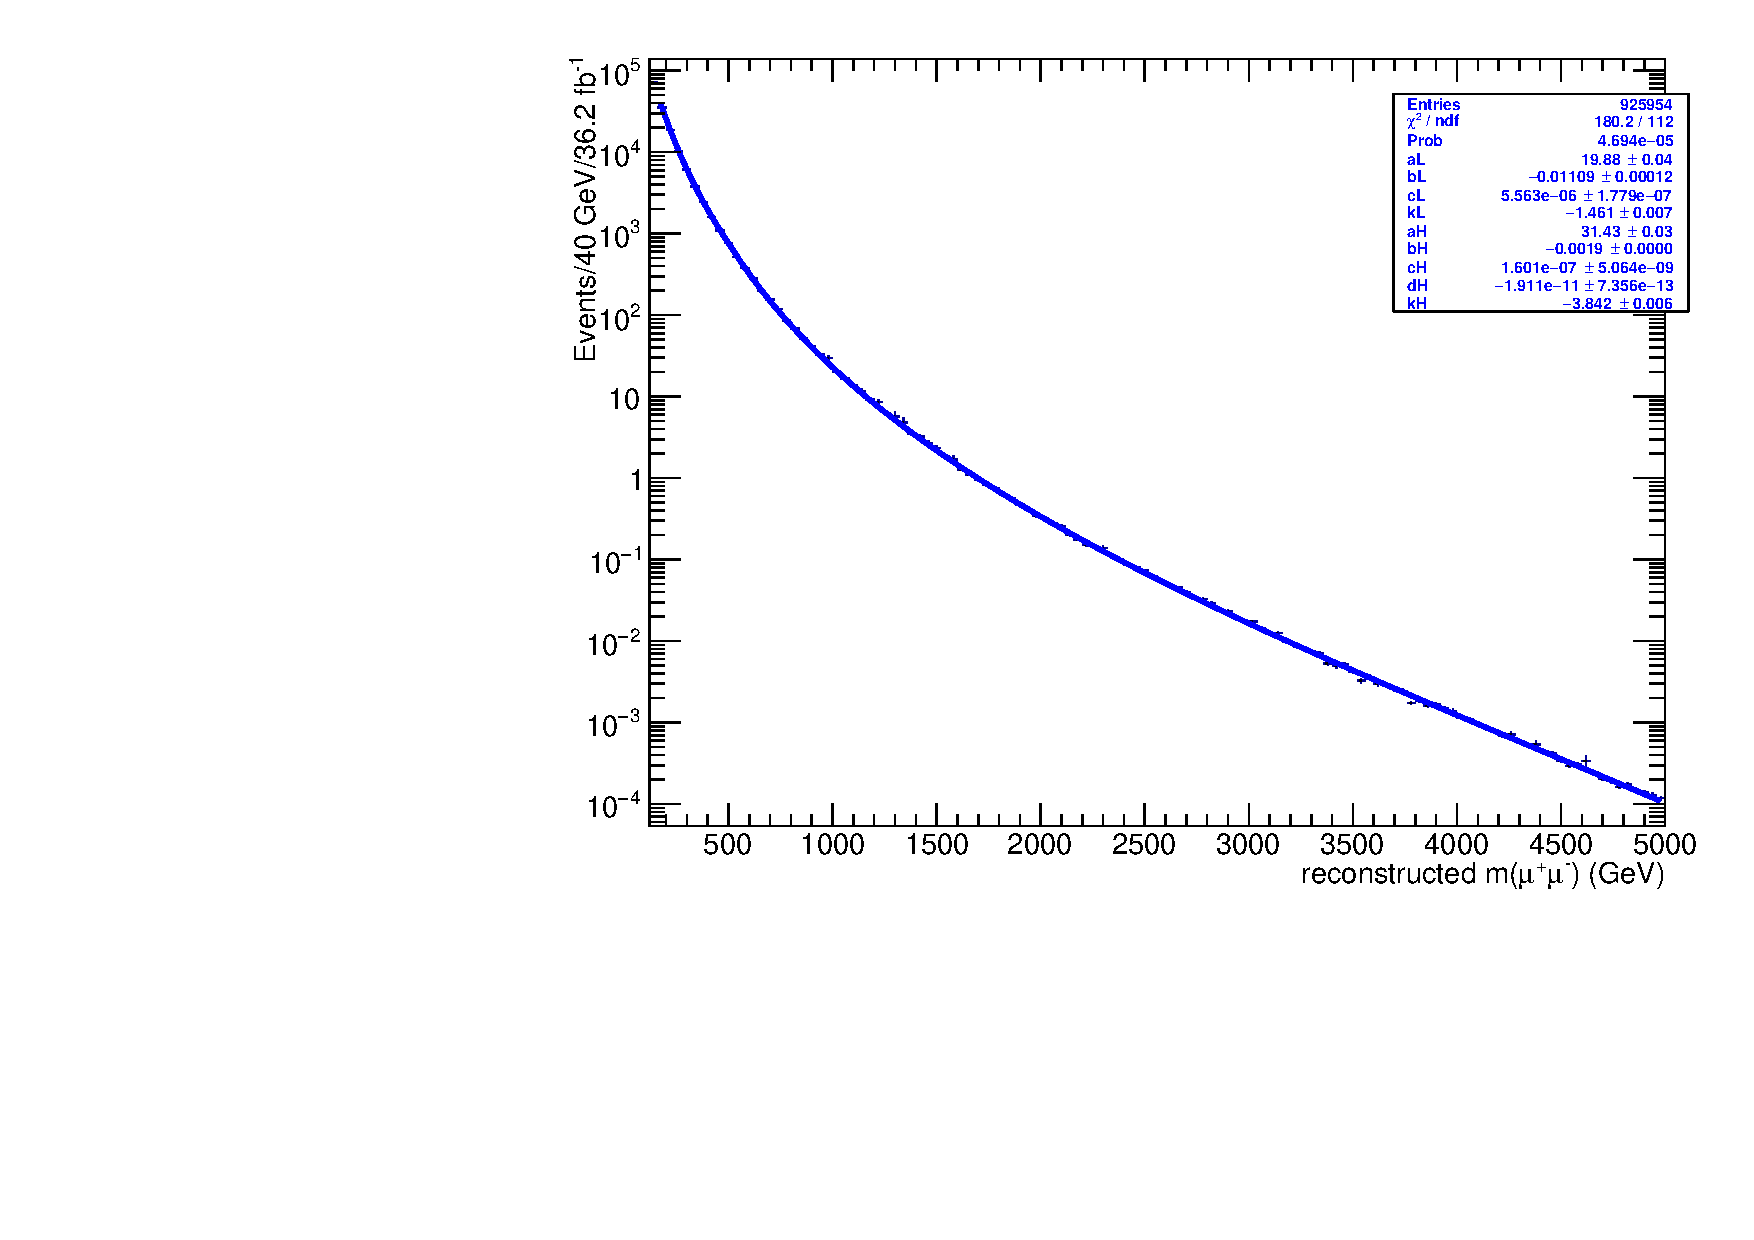
\includegraphics[width=0.47\textwidth]{Images/Cap5/mass150_5000_log_BE_9par.pdf}
\caption{\label{bkg_fit} Fit of the background shape for different $\eta$ categories: BB category on the left, BE category  on the right.}
\end{figure}

\begin{figure}[htbp]
\centering
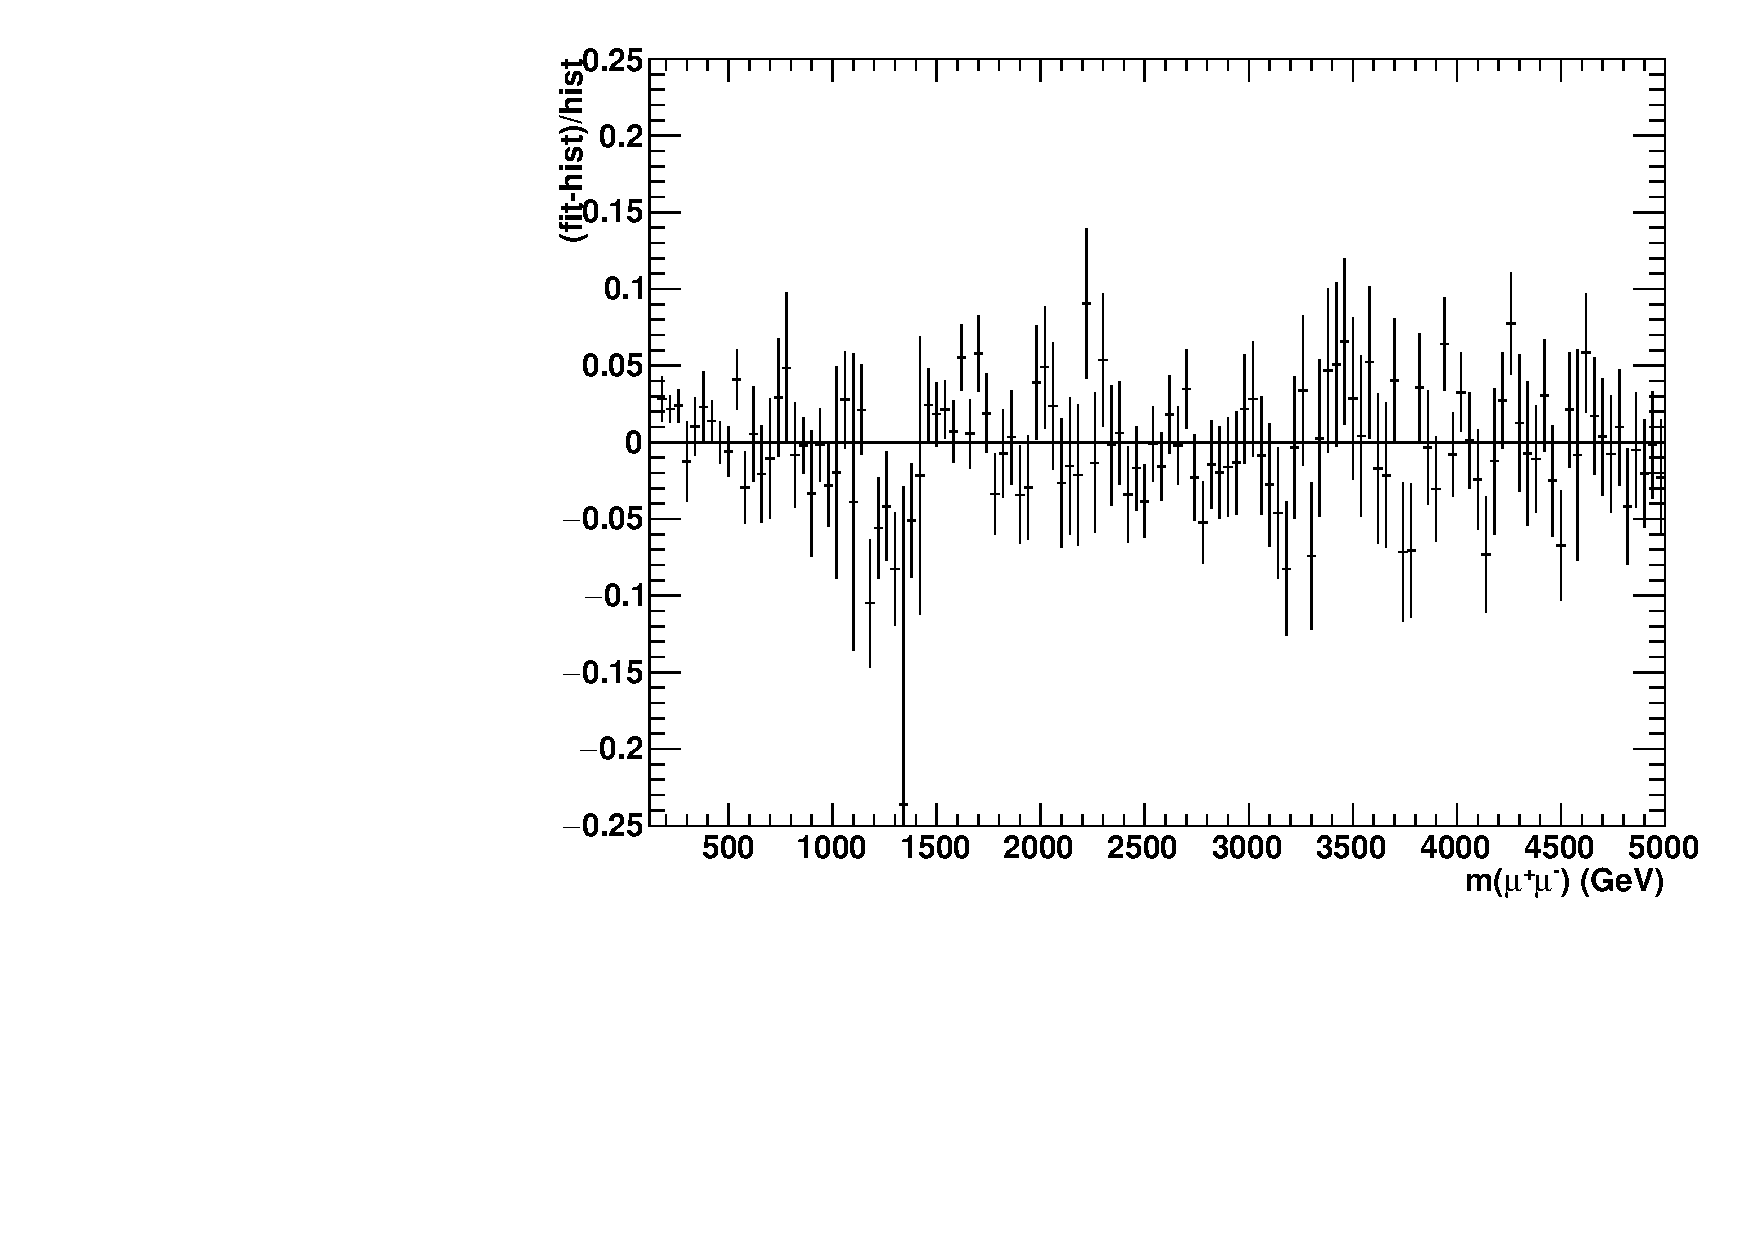
\includegraphics[width=0.4\textwidth]{Images/Cap5/res_150_5000_BB_9par.pdf}
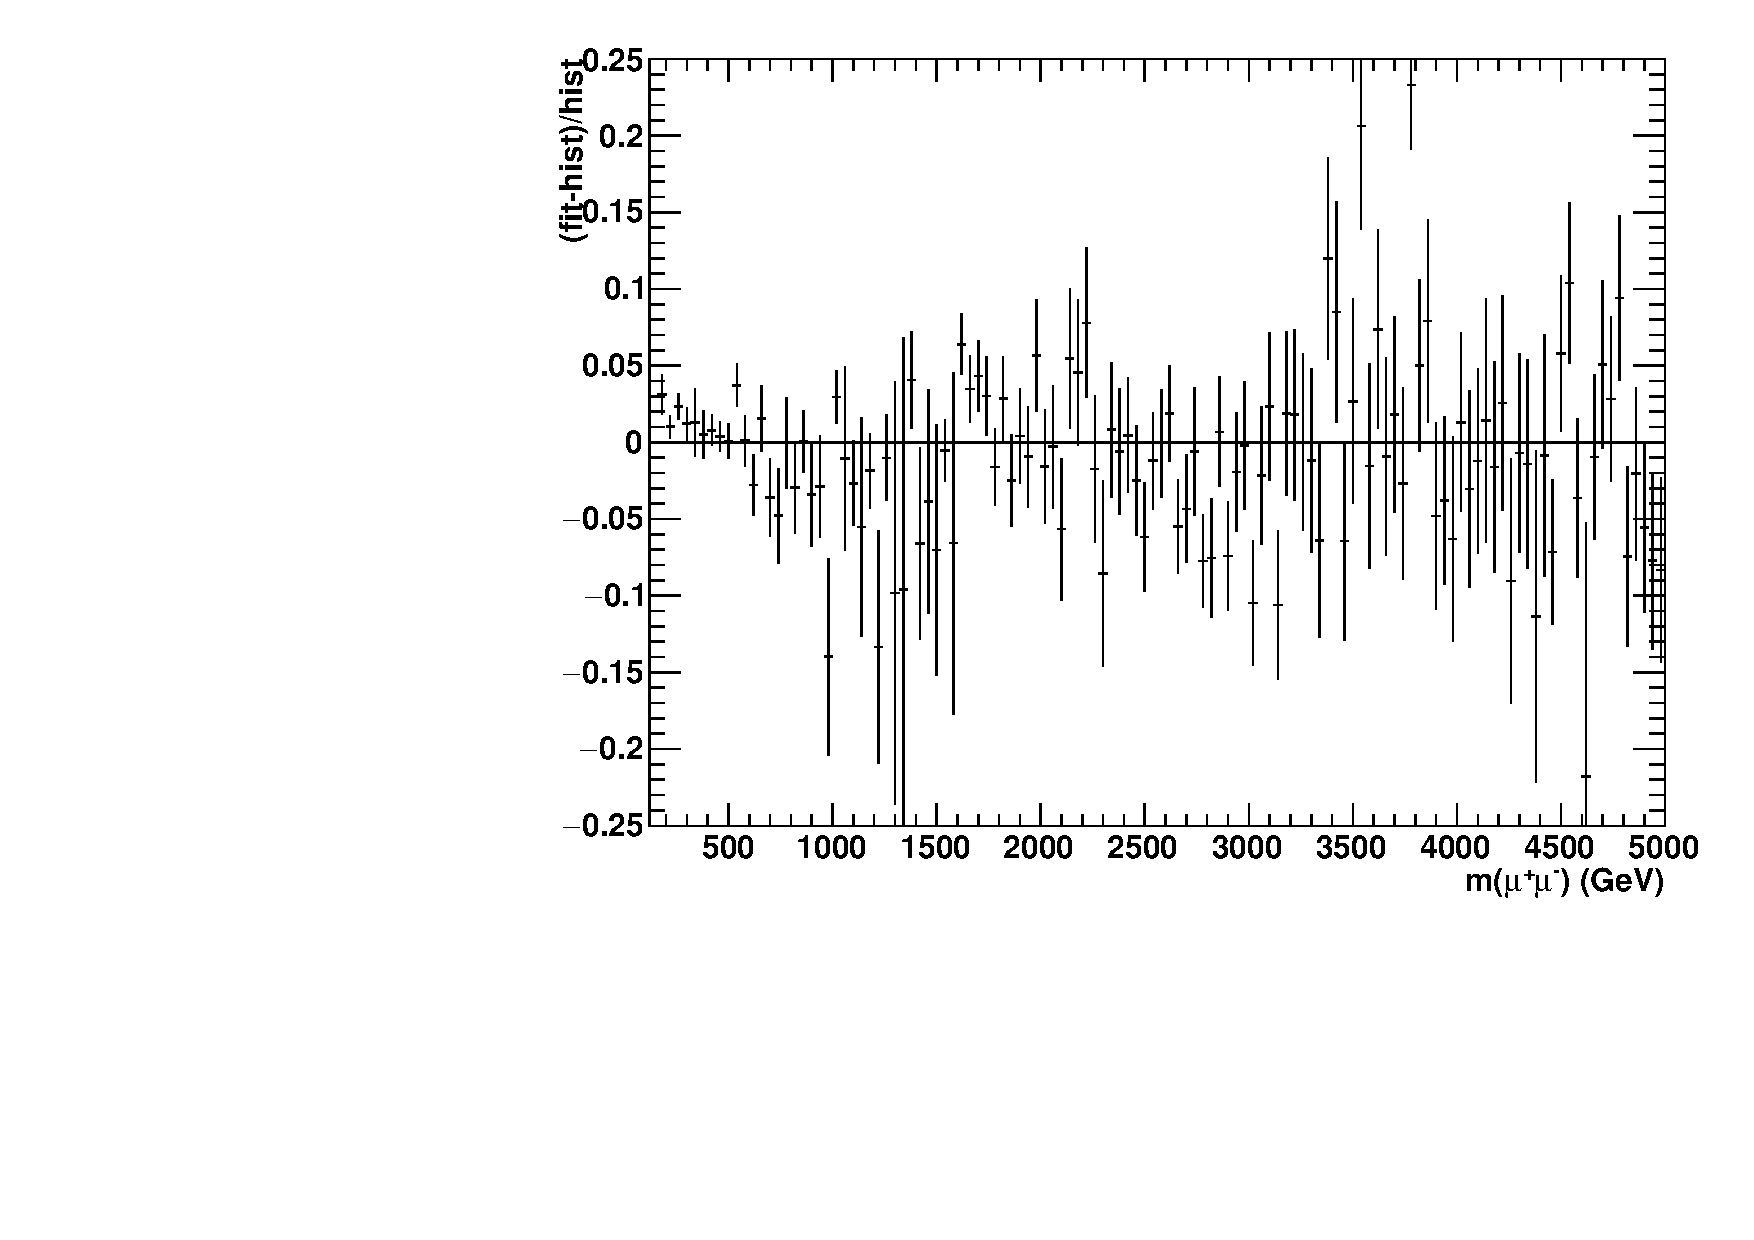
\includegraphics[width=0.4\textwidth]{Images/Cap5/res_150_5000_BE_9par.pdf}
\caption{\label{fig:bkg_res} Residual of the fits for different $\eta$ categories: BB category on the left, BE category on the right.}
\end{figure}

\section{Statistical analysis}
In the absence of a signal, limits are set on the ratio $R_{\sigma}$ of the production cross section times branching fraction for high-mass resonances to that for the Z boson:
\begin{equation}
R_\sigma = \frac{\sigma(pp\to Z'+X\to\mm+X)}{\sigma(pp\to Z+X\to\mm+X)} =
\frac{ N(Z'\to\mm) }{N(Z\to\mm)} \times \frac{ A(Z\to\mm)}{ A(Z'\to\mm) } \times \frac{ \varepsilon(Z\to\mm) }{\varepsilon(Z'\to\mm)}\,,
\label{eqn:r}
\end{equation}
where $N$ is the number of events, $A$ is the detector acceptance, and $\varepsilon$ is the total selection efficiency. $N(Z\to\mm)$ 
of Z events for normalization to the Z cross section is evaluated changing some requirements described in section \ref{sec:selection}: in particular, with trigger \texttt{HLT\_Mu(Tk)50} and requiring the offline muon \pt at least 53 GeV, the number of the Z events would be reduced by roughly two orders of magnitude and would give a different kinematics than the original Z production, leading to a problem with systematic uncertainties of the procedure. Therefore, the prescaled triggers \texttt{HLT\_Mu(Tk)27} and a correspondingly reduced value of 30~GeV for the \pt cut for the offline muon are used. This trigger had different values of prescale factors at different runs and luminosity sections during the data taking. In order to enlarge the statistics at the Z peak which is used for the Z-peak normalization, the whole sample was divided into sub-samples with different prescale factors and different integrated luminosity for each $\eta$ category defined (see \tablename~\ref{tab:prescale_lumi}). The mean \texttt{HLT\_Mu27} prescale rate in the data was found to be $1/167.737$. \\
The whole data has been divided into four periods according to the level of improvement of the trigger, alignment and the HIP issue, see \tablename~\ref{tab:periods}.
Period 1 was the initial data taking till Summer 2016; in period 2 new alignment and calibration constants were deployed (derived on June dataset); in period 3 Muon L1 issues were fixed.
and finally in period 4 the so-called ``HIP inefficiency"' (also known as ``SiStrip dynamic inefficiency'') for high instantaneous lumi was solved.

\begin{table}[htb!]
\begin{center}
\scalebox{0.83}{\begin{tabular}{|r|r|l|l|l|l|l|}
\hline
%%%%%%%%%%%%%%%%%%%%%%%%%%%%%%%%%%%%%%%%%%%%%%%%%%%%%%%%%%%%%%%%%%%%%%%%%%%%%%%%%%%%%%%%%%%%%
\multicolumn{1}{|c|}{Prescale} & Int. lumi,& \multicolumn{3}{c|}{Ratio Data / MC, for different categories} \\ \cline{3-5}
\multicolumn{1}{|c|}{factor} & pb$^{-1}$\hspace*{1.0em} & \multicolumn{1}{c|}{\bf All} & \multicolumn{1}{c|}{\bf BB}  & \multicolumn{1}{c|}{\bf BE\,+\,EE} \\ \hline
% Prescale               &                      & Category 0            & Category 1            & Category 2
%%%%%%%%%%%%%%%%%%%%%%%%%%%%%%%%%%%%%%%%%%%%%%%%%%%%%%%%%%%%%%%%%%%%%%%%%%%%%%%%%%%%%%%%%%%%%
     14  \hspace*{1.0em} &    11\hspace*{1.0em} & $0.9573 \pm 0.0490$ & $0.9484 \pm 0.0755$ & $0.9637 \pm 0.0645$  \\ \hline
     35  \hspace*{1.0em} &    59\hspace*{1.0em} & $1.0383 \pm 0.0344$ & $0.9934 \pm 0.0521$ & $1.0708 \pm 0.0459$  \\ \hline
     40  \hspace*{1.0em} &    48\hspace*{1.0em} & $0.9500 \pm 0.0391$ & $0.9486 \pm 0.0604$ & $0.9511 \pm 0.0513$  \\ \hline
     70  \hspace*{1.0em} &  1455\hspace*{1.0em} & $0.9738 \pm 0.0096$ & $0.9639 \pm 0.0147$ & $0.9812 \pm 0.0126$  \\ \hline
    100  \hspace*{1.0em} &  7065\hspace*{1.0em} & $0.9809 \pm 0.0052$ & $0.9807 \pm 0.0080$ & $0.9815 \pm 0.0068$  \\ \hline
    120  \hspace*{1.0em} &   479\hspace*{1.0em} & $0.9890 \pm 0.0220$ & $0.9995 \pm 0.0342$ & $0.9822 \pm 0.0288$  \\ \hline
    140  \hspace*{1.0em} &  4516\hspace*{1.0em} & $0.9864 \pm 0.0077$ & $0.9850 \pm 0.0118$ & $0.9883 \pm 0.0101$  \\ \hline
    150  \hspace*{1.0em} &  4828\hspace*{1.0em} & $0.9428 \pm 0.0075$ & $0.9370 \pm 0.0116$ & $0.9479 \pm 0.0099$  \\ \hline
    160  \hspace*{1.0em} &  2738\hspace*{1.0em} & $0.9856 \pm 0.0105$ & $0.9931 \pm 0.0163$ & $0.9811 \pm 0.0138$  \\ \hline
    170  \hspace*{1.0em} &  3081\hspace*{1.0em} & $0.9187 \pm 0.0099$ & $0.9471 \pm 0.0155$ & $0.8993 \pm 0.0128$  \\ \hline
    180  \hspace*{1.0em} &   518\hspace*{1.0em} & $1.0002 \pm 0.0261$ & $1.0209 \pm 0.0407$ & $0.9865 \pm 0.0340$  \\ \hline
    200  \hspace*{1.0em} &  3719\hspace*{1.0em} & $0.9327 \pm 0.0098$ & $0.9408 \pm 0.0152$ & $0.9280 \pm 0.0128$  \\ \hline
    230  \hspace*{1.0em} &  3299\hspace*{1.0em} & $0.9479 \pm 0.0112$ & $0.9696 \pm 0.0176$ & $0.9337 \pm 0.0146$  \\ \hline
    250  \hspace*{1.0em} &  1010\hspace*{1.0em} & $0.9510 \pm 0.0214$ & $0.9794 \pm 0.0335$ & $0.9321 \pm 0.0277$  \\ \hline
    260  \hspace*{1.0em} &  2345\hspace*{1.0em} & $0.9447 \pm 0.0141$ & $0.9857 \pm 0.0223$ & $0.9168 \pm 0.0183$  \\ \hline
    290  \hspace*{1.0em} &  1828\hspace*{1.0em} & $0.9481 \pm 0.0169$ & $0.9556 \pm 0.0263$ & $0.9446 \pm 0.0222$  \\ \hline
    320  \hspace*{1.0em} &   196\hspace*{1.0em} & $0.9387 \pm 0.0540$ & $0.9145 \pm 0.0825$ & $0.9581 \pm 0.0716$  \\ \hline
    320  \hspace*{1.0em} &   196\hspace*{1.0em} & $0.9387 \pm 0.0540$ & $0.9145 \pm 0.0825$ & $0.9581 \pm 0.0716$  \\ \hline
%%%%%%%%%%%%%%%%%%%%%%%%%%%%%%%%%%%%%%%%%%%%%%%%%%%%%%%%%%%%%%%%%%%%%%%%%%%%%%%%%%%%%%%%%%%%%
\hline
Combined                 & 36295\hspace*{1.0em} & $0.9638 \pm 0.002$ &  $0.9688 \pm 0.0042$ & $0.9610 \pm 0.0035$  \\ \hline
%%%%%%%%%%%%%%%%%%%%%%%%%%%%%%%%%%%%%%%%%%%%%%%%%%%%%%%%%%%%%%%%%%%%%%%%%%%%%%%%%%%%%%%%%%%%%
\end{tabular}}
\caption{\label{tab:prescale_lumi}
Integrated luminosities for different prescale factors of prescaled triggers \texttt{HLT\_(Tk)Mu27} for two categories.
}
\end{center}
\end{table}

\begin{table}[htb!]
\scalebox{0.93}{\small
\begin{tabular}{|c|l|c|r|c|c|c|c|c|c|}
\hline
No. & Run era    & Run range & \multicolumn{3}{c|}{{\cal L}, fb$\boldmath^{-1}$} & ``Calib'' & ``Trig'' & ``HIP''\\ \cline{4-7}
    &            &                        & Nov. 2016 & Jan. 2017 & Feb. 2017    &           &          &        \\ \hline
1   & B + C + D  & 273\,150 --- 276\,811  & 13.081    & 13.081    & 12.754       & ---       & ---      & ---    \\ \hline
2   & E + F      & 276\,831 --- 278\,167  &  4.753    &  4.835    &  4.709       & +         & ---      & ---    \\ \hline
3   & F          & 278\,175 --- 278\,801  &  2.078    &  2.084    &  2.028       & +         & +        & ---    \\ \hline
4   & F + G + H  & 278\,802 --- 284\,044  & 16.722    & 17.196    & 16.747       & +         & +        & +      \\ \hline
\end{tabular}}
\caption{\label{tab:periods}
Used run periods.
}
\end{table}
%By taking the ratio of observed events at higher masses to events in the normalization region, the dependence on experimental acceptance, trigger and offline efficiencies is eliminated at lowest order, leaving only a residual dependence on the variation of these quantities with invariant mass. The impact of PDF uncertainty on the results is also reduced in this approach.

\section{Dimuon mass and Data-MC comparison}
In \figurename~\ref{mass_plot} the comparison between data and simulation for the dimuon invariant mass spectrum over the full pseudorapidity range is shown. All the dimuon mass plots are corrected for the corresponding data/MC ($R_Z$) ratio found at Z peak in \tablename~\ref{tab:prescale_lumi}. In \figurename~\ref{mass_plot_cat} invariant mass plots distributions for different categories of pseudorapidity are shown.

\begin{figure}[htbp]
\centering
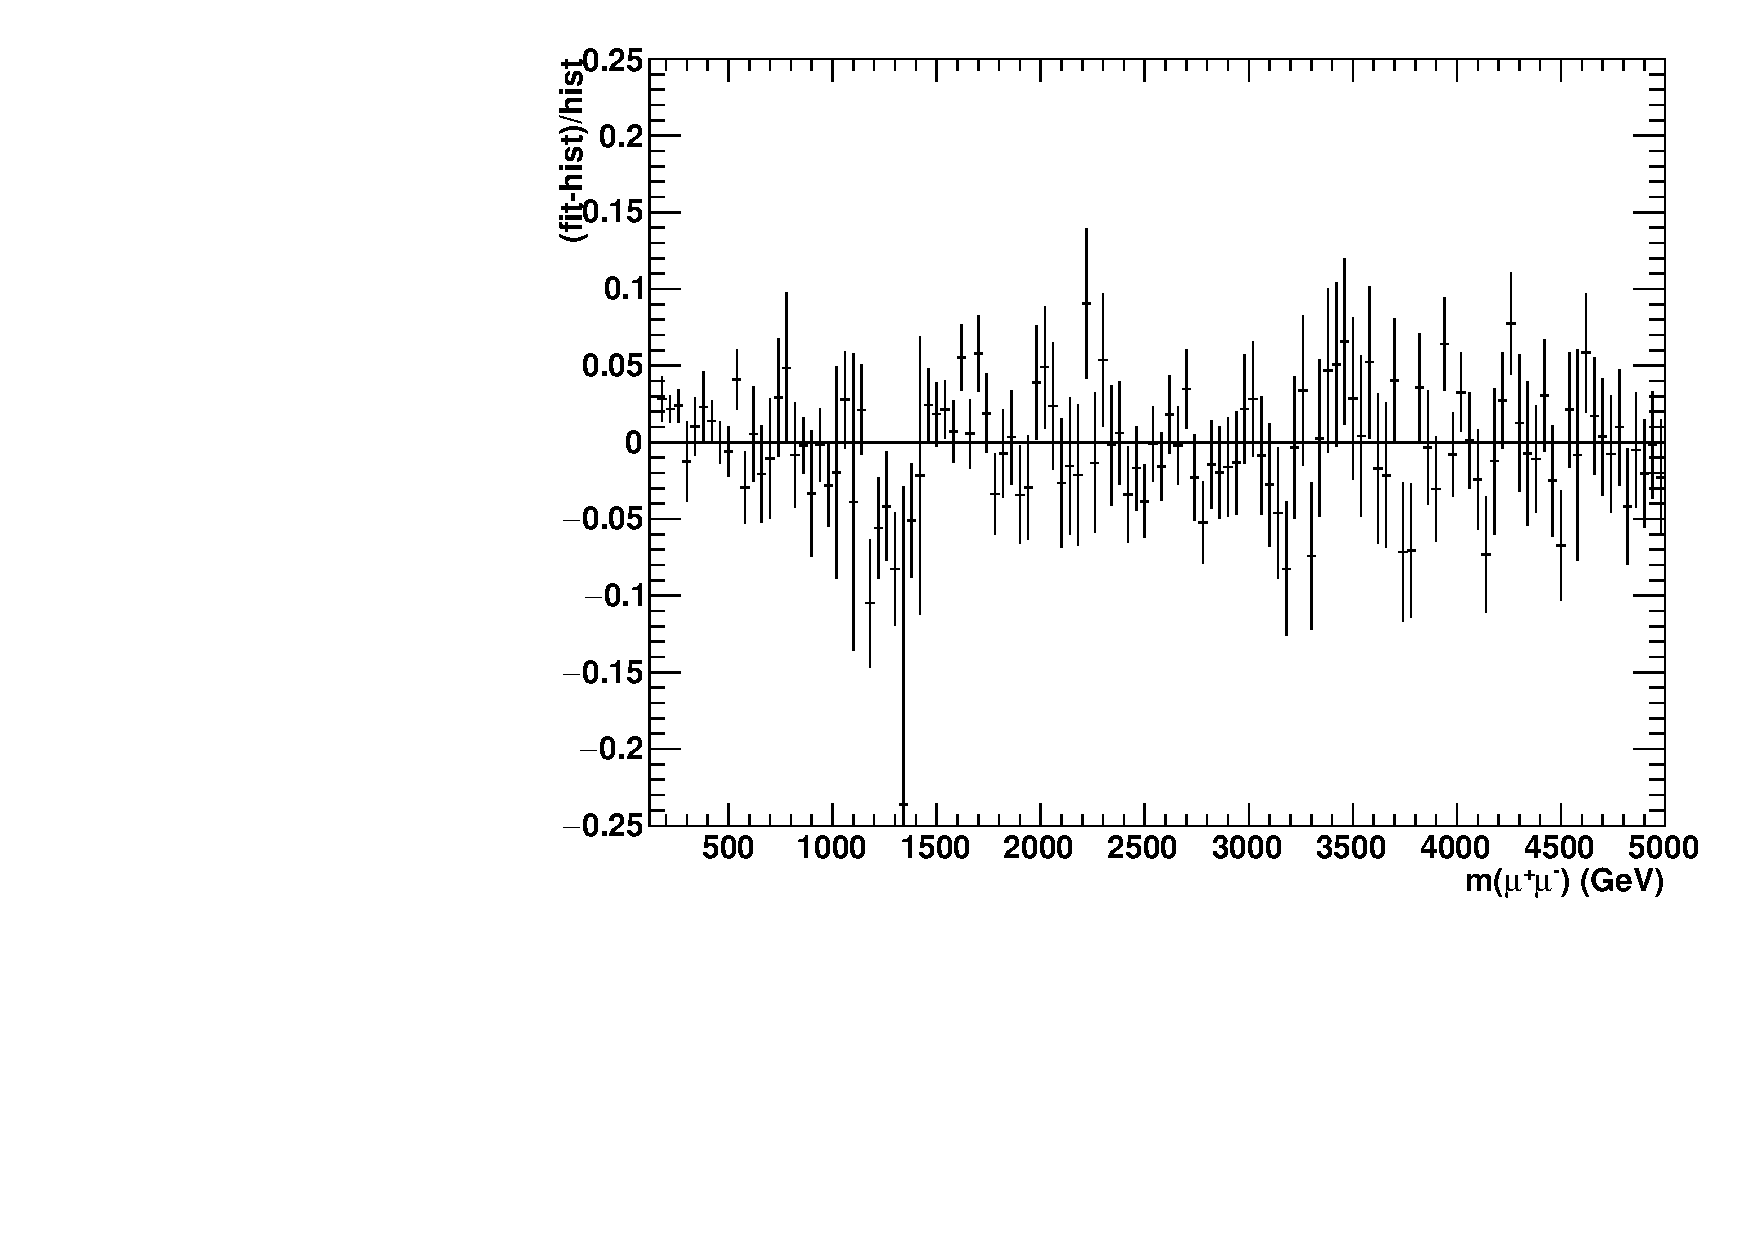
\includegraphics[width=0.1\textwidth]{Images/Cap5/res_150_5000_BB_9par.pdf}
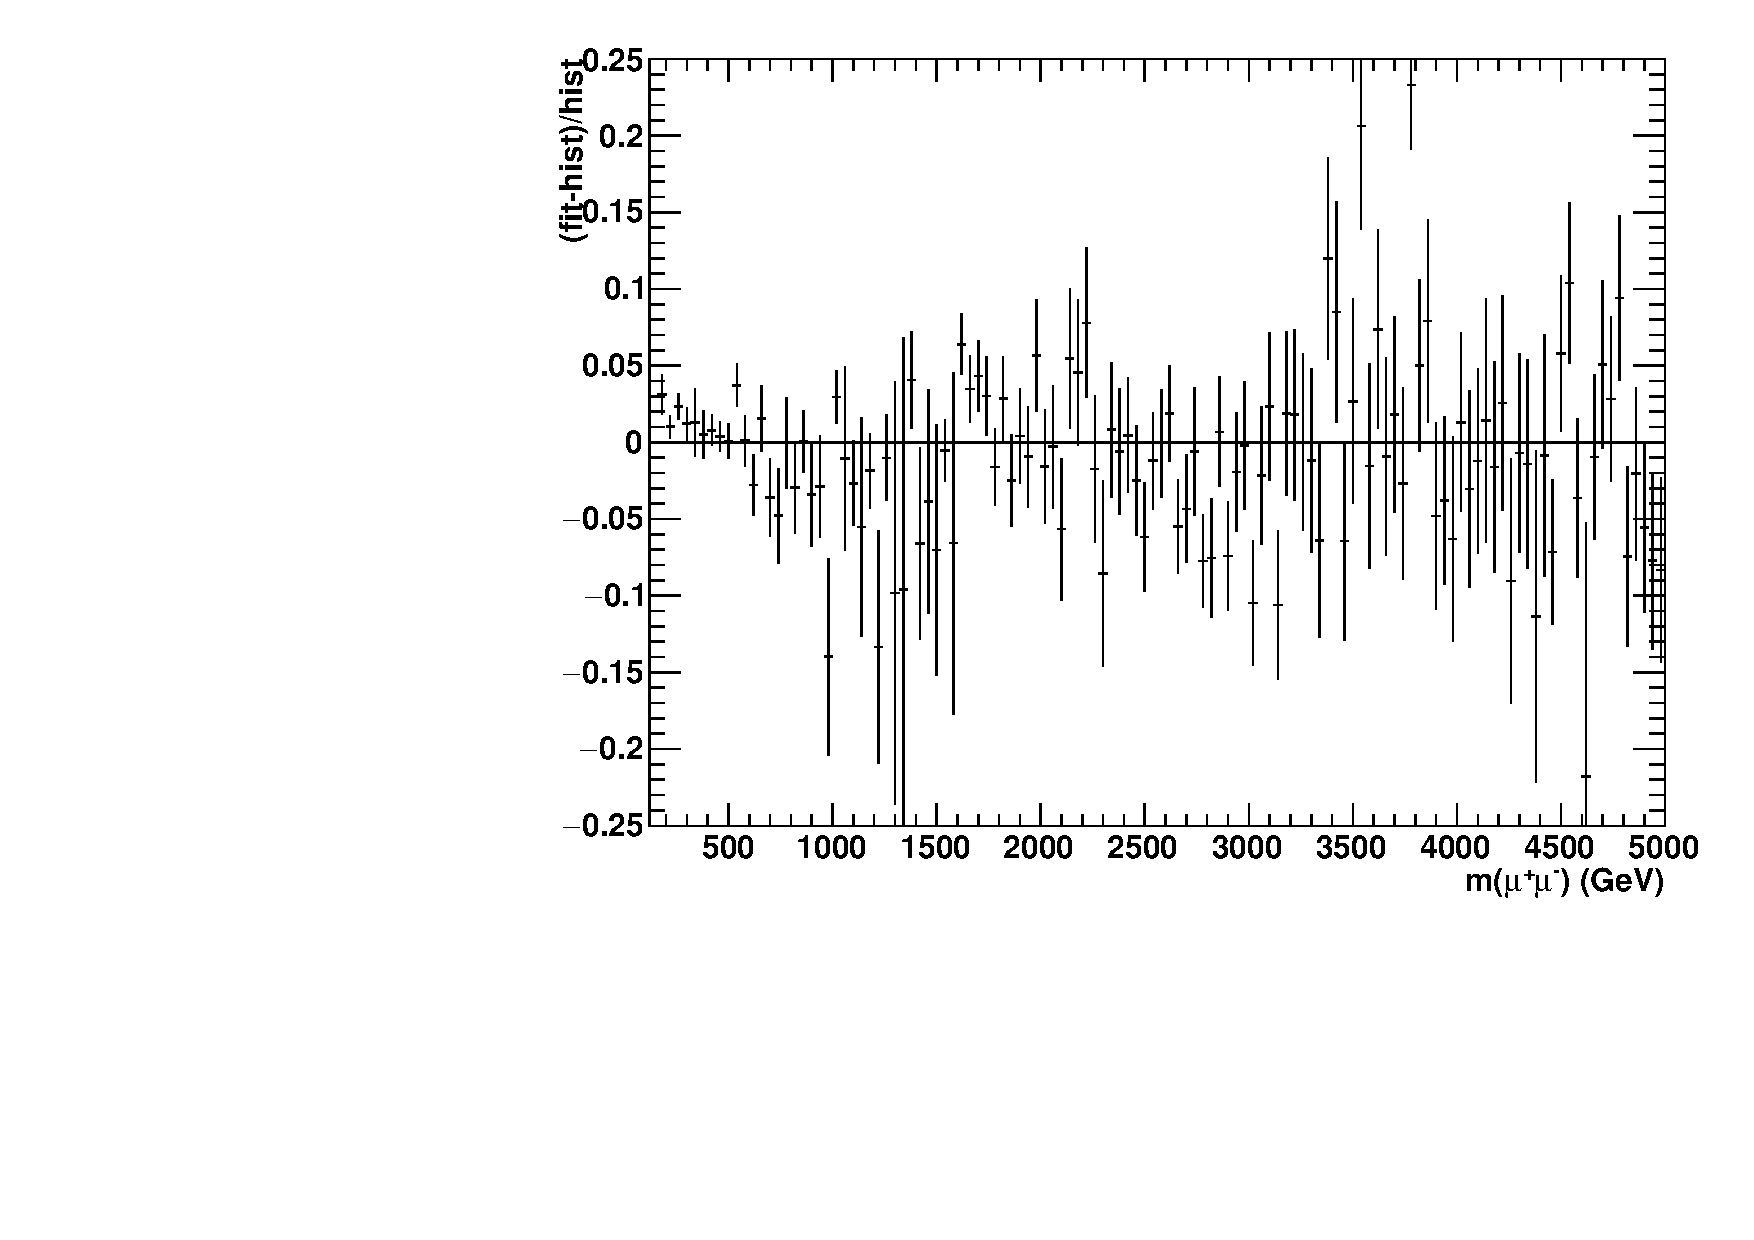
\includegraphics[width=0.1\textwidth]{Images/Cap5/res_150_5000_BE_9par.pdf}
\caption{The observed invariant mass spectra, together with the predicted SM backgrounds (on the right the cumulative one).}
\label{mass_plot} 
\end{figure}

\begin{figure}[htbp]
\centering
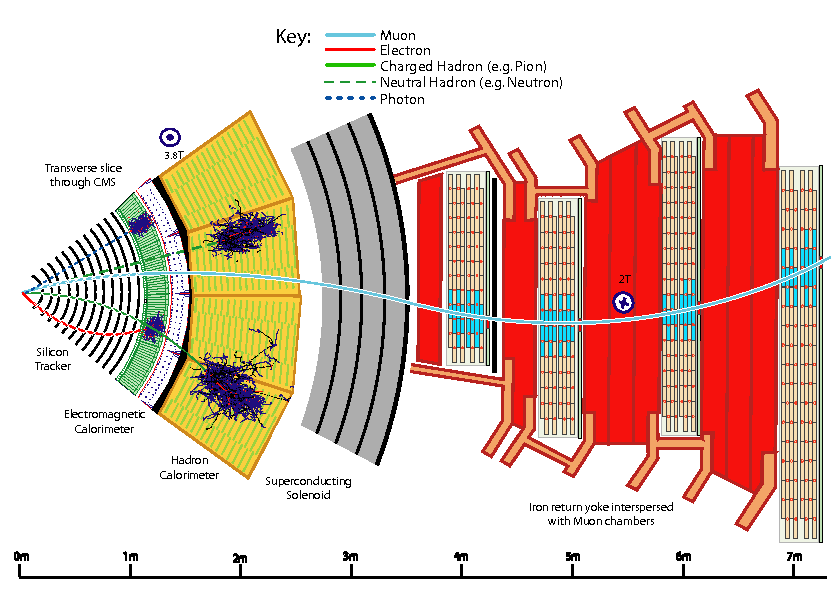
\includegraphics[width=0.1\textwidth]{Images/ParticleFlow}
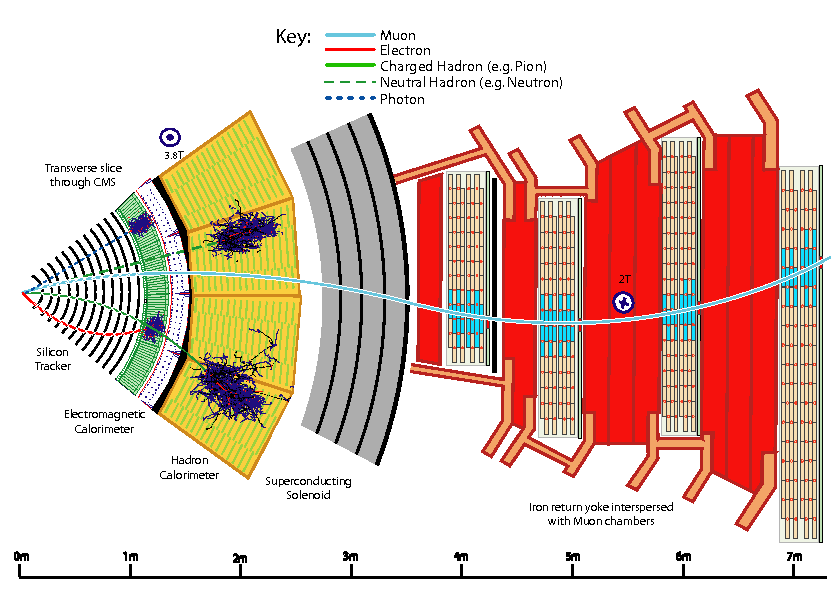
\includegraphics[width=0.1\textwidth]{Images/ParticleFlow}
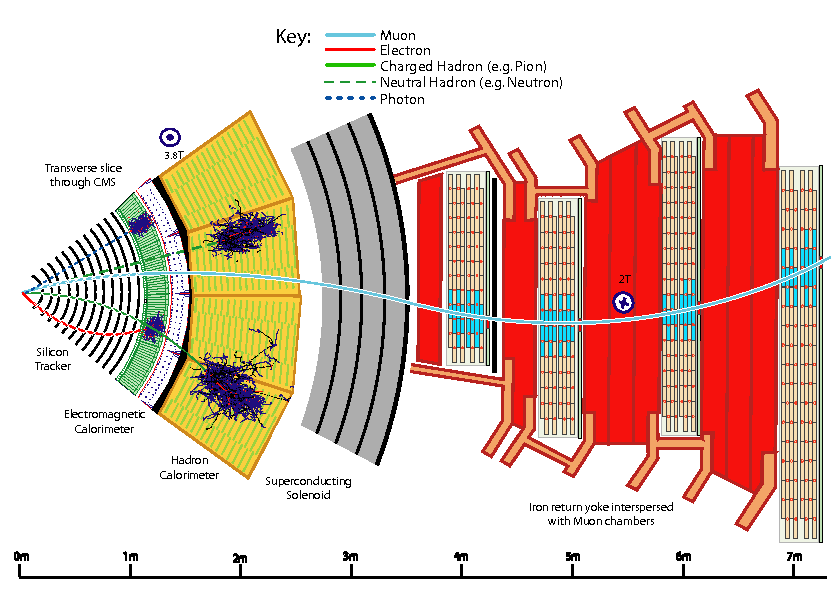
\includegraphics[width=0.1\textwidth]{Images/ParticleFlow}
\includegraphics[width=0.1\textwidth]{Images/ParticleFlow}
\caption{The observed invariant mass spectra, together with the predicted SM backgrounds: on top for BB category and on bottom for BE (on the right column, the cumulative ones).}
\label{mass_plot_cat}
\end{figure}

\begin{comment}
Above 700 GeV in the barrel-barrel $\eta$ category we observe a deficit in data compare to MC predictions that is currently investigated.

\figurename~\ref{fig:zprime_public_style} and \ref{fig:zprime_public_style_green} show the same distributions in a style prepared for the paper. 
They show also systematic uncertainties for the spectrum of dimuon invariant mass with the following sources summed quadratically:
\begin{itemize}
\item $A\times\varepsilon$ vs $M$ ~with reweighting MC events giving ~3.3\,\% for $M=4$~TeV (this uncertainty is considered only in the downward direction).
\item Contribution from mass resolution and scale used the function for fitting second-order polynomial:\\
$s = \left|-0.001792 + 2.484 \times 10^{-6} \,M -4.795\times 10^{-9} \,M^2\right|$\\  
which describes uncertainties from scale correction to inclusive mass spectrum,
giving estimate for this systematic uncertainty 6.9\,\% for $M=4$~TeV.
\item Normalization to Z peak: 1\,\% uncertainty is considered on the normalization factor estimated from Z peak.
\item Drell-Yan uncertainty is calculated from fit of points in Table 11 of AN-16-053 snapshot:\hspace*{-25mm}~\\
$\mbox{pdf} = 6.68537\cdot 10^{-3} + 2.54218\cdot 10^{-5} M - 1.09503\cdot 10^{-8}M^2 + 1.97141\cdot 10^{-12} M^3,$\\
where $M$ is dimuon mass in GeV.
\item 7\,\% uncertainty of the cross section of the Non-DY background estimated from MC for different processes.
\item 50\,\% uncertainty of fake rate jet estimate.
\item Trigger efficiency using systematic uncertainty from trigger efficiency 0.3\% in the BB and 0.7\% in the BE category (Section~\ref{sec:sys})
combined with fractions of BB and BE categories as functions of mass,
which gives result 0.46--0.57 \% depending on the mass.
\end{itemize}

\begin{figure}[!h]
  \begin{center}
    \includegraphics[width=0.70\textwidth]{AnalysisStrategy/fig/zprime_style_syst.pdf}
\\
    \includegraphics[width=0.70\textwidth]{AnalysisStrategy/fig/zprime_style_syst_cumul.pdf}
    \caption{ The observed opposite-sign dimuon invariant mass spectrum, overlaid on the background prediction from simulation,
       differential (top) and cumulative (bottom) plots, in a style prepared for the paper.
      % with the Di-jet and the W+jets contribution coming from data driven estimate.
      % ``Other prompt leptons'' and ``jets'' are as described in Fig.~\ref{fig:mass_plot}.
      }
    \label{fig:zprime_public_style}
  \end{center}
\end{figure}

\begin{figure}[!h]
  \begin{center}
    \includegraphics[width=0.70\textwidth]{AnalysisStrategy/fig/zprime_style_syst_green.pdf}
\\
    \includegraphics[width=0.70\textwidth]{AnalysisStrategy/fig/zprime_style_syst_cumul_green.pdf}
    \caption{ The observed opposite-sign dimuon invariant mass spectrum which differs from the previous figure by a different grouping of backgrounds
       which was used in CMS paper \cite{Khachatryan:2016zqb} and PAS \cite{CMS:2016abv}.
      }
    \label{fig:zprime_public_style_green}
  \end{center}
\end{figure}

\begin{figure}[htbp]
\centering
\includegraphics[width=0.1\textwidth]{Images/ParticleFlow}
\includegraphics[width=0.1\textwidth]{Images/ParticleFlow}
\includegraphics[width=0.1\textwidth]{Images/ParticleFlow}
\includegraphics[width=0.1\textwidth]{Images/ParticleFlow}
\caption{The observed opposite-sign dimuon invariant mass spectrum, overlaid on the background prediction from simulation, in log (left) and linear (right) scale. Top row is for dimuons from barrel-barrel category, and bottom one is for dimuons from barrel-endcap and endcap-endcap category.}
\label{fig:mass_plot_cat}
\end{figure}

\begin{figure}[htbp]
\centering
\includegraphics[width=0.1\textwidth]{Images/ParticleFlow}
\includegraphics[width=0.1\textwidth]{Images/ParticleFlow}
\includegraphics[width=0.1\textwidth]{Images/ParticleFlow}
\includegraphics[width=0.1\textwidth]{Images/ParticleFlow}
\caption{The observed opposite-sign cumulative dimuon invariant mass spectrum, overlaid on the background prediction from simulation, in log (left) and linear (right) scale. Top row is for dimuons from barrel-barrel category, and bottom one is for dimuons from barrel-endcap and endcap-endcap category.}
\label{fig:mass_plot_cat_cumul}
\end{figure}

\begin{figure}[!h]
  \begin{center}
    \includegraphics[width=0.49\textwidth]{AnalysisStrategy/fig/datamc_log_mass_cumul_period1.pdf}\put(-170,160){\bf\large (1)}
    \includegraphics[width=0.49\textwidth]{AnalysisStrategy/fig/datamc_log_mass_cumul_period2.pdf}\put(-170,160){\bf\large (2)}
\\
    \includegraphics[width=0.49\textwidth]{AnalysisStrategy/fig/datamc_log_mass_cumul_period3.pdf}\put(-170,160){\bf\large (3)}
    \includegraphics[width=0.49\textwidth]{AnalysisStrategy/fig/datamc_log_mass_cumul_period4.pdf}\put(-170,160){\bf\large (4)}
    \caption{Number of opposite-sign dimuons with invariant mass
      greater than the given value, overlaid on the background prediction
      from simulation, in log scale, for four periods of 2016 data taking defined in Table\,\ref{tab:periods}.}
    \label{fig:mass_plot_cumul_periods}
  \end{center}
\end{figure}
\end{comment}

The comparison between data and simulation for different variables is shown in \figurename~\ref{Variables_DataMC}.
\begin{figure}[htbp]
\centering
\includegraphics[width=0.1\textwidth]{Images/ParticleFlow}
\includegraphics[width=0.1\textwidth]{Images/ParticleFlow}
\includegraphics[width=0.1\textwidth]{Images/ParticleFlow}
\includegraphics[width=0.1\textwidth]{Images/ParticleFlow}
\caption{Data-MC comparison.}
\label{Variables_DataMC} 
\end{figure}


\section{Signal parametrization}
\subsection{Signal acceptance and efficiency}
Using DY samples from 50 to 6000 GeV, the combined reconstruction and selection efficiency, for dimuon passing the selection defined in section \ref{sec:selection}, as a function of dimuon mass itself, has been evaluated and reported in \figurename~\ref{EffAcc}. 
%the efficiency with respect to events in the acceptance (defined as both muons in $-2.4<\eta<2.4$ and \pt $ > 53$ GeV) is shown in red while the total acceptance times efficiency in blue. The acceptance as a function of the mass is shown in green. 
%The overall acceptance and efficiency is produced for two categories corresponding to the location of the two muons as defined in section~\ref{sec:etaCategory}.
%The fit of the acceptance times efficiency is used to parametrize the Z$`$ acceptance and efficiency.

\begin{figure}[htbp]
\centering
\includegraphics[width=0.47\textwidth]{Images/Cap5/AccEff_BB.pdf}
\includegraphics[width=0.47\textwidth]{Images/Cap5/AccEff_BE.pdf}
\includegraphics[width=0.47\textwidth]{Images/Cap5/AccEff_All.pdf}
\caption{The combined reconstruction and selection efficiency, as a function of the invariant mass, for dimuon passing the selection (section \ref{sec:selection}) with respect to all events in acceptance (red), the total acceptance times efficiency (blue), and the acceptance (green), as evaluated on simulated Drell-Yan events: on top left for BB category, on top right for BE and on the bottom for the inclusive $\eta$ range. Also shown are the fit functions to the acceptance times efficiency for the two categories and integrated in pseudo-rapidity.}
\label{EffAcc}
\end{figure}

These acceptance $\times$ efficiency values are valid for spin-1 resonances. For the interpretation of the analysis in spin-2 models, it is calculated using the RS Graviton signal samples. The muons from the decay of the resonance are more central, the efficiency is higher in the BB category and slightly lower in the BE category. The overall efficiency is higher compared to spin-1 resonances. The resulting efficiency curves are shown in \figurename~\ref{EffAccSpin2}.

\begin{figure}[htbp]
\centering
\includegraphics[width=0.4\textwidth]{Images/Cap5/AccEff_BB_RS.pdf}
\includegraphics[width=0.4\textwidth]{Images/Cap5/AccEff_BE_RS.pdf}
\caption{The combined reconstruction and selection efficiency, as a function of the invariant mass, for dimuons passing our selection for the case of spin-2 resonances. Shown is the total acceptance $\times$ efficiency with respect to all generated events. The efficiencies are fitted with the same functions as int the spin-1 case.}
\label{EffAccSpin2}
\end{figure}

\begin{comment}
MC efficiency predictions could overestimate the data efficiency in
particular when going at high masses. At low pT corrections to applied
on MC to match the data are derived using Z signal but they can't
be safely progagated to high pT without checking that the observed
data to MC difference is not getting worse with pT. Dedicated methods
have been developped to masured the single muon ID and Reco
efficiencies in data as a function of pT (or p) in sections 5.3 and
4.2, respectively. It appears that the standalone reconstruction and
the number of standalone/global valid hits become less efficient at
high pT (or p) in the forward part of the detector ($1.6<|\eta|<2.4$) and that MC is not able to reproduce the observed
trend (see figure \ref{fig_reco_f}, right plot). On the other hand the inefficiency measured in data for both the
Id and reconstruction with respect to simulation, is found to be
constant as a function of pT (or p) for $0<|\eta|<1.6$ (see figure \ref{fig_reco_f}, left plot). These data to
MC comparisons are only valid up to 2 TeV in p and a systematic needs
to be applied on the above mass parametrization that extend till 5
TeV.
\end{comment}

These results are corrected for the single muon ID and Reco efficiencies in data \ref{sec:IDefficiency}, applying a weight for each muon: the weight depends on the muon p and on the muon $\eta$. The new efficiencies $\times$ acceptance parametrisation obtained from DY simulation as a function of mass are displayed on figure \ref{Effsys}. The ratio between the nominal one (weight = 1, black curve) and the new parametrisation (red curve) is taken as systematic on the signal efficiency. 

\begin{figure}[htbp]
\centering
\includegraphics[width=0.45\textwidth]{Images/Cap5/BarrelEffSysFinal}
\includegraphics[width=0.45\textwidth]{Images/Cap5/EndcapEffSysFinal}
\caption{Shown is the acceptance $\times$ efficiency as a function of mass obtained after applying the weights on single muon (p, $\eta$) coming from the Id+Reco study in section 4.2.}
\label{Effsys}
\end{figure}

\subsection{Mass resolution}
Mass experimental resolution is determined from DY simulation as a function of the generated dimuon mass in each of the pseudorapidity categories (BB and BE). For each considered mass bin, the residual has been measured comparing the reconstructed mass with the generated one: each residual is then fit using Cruijff function, the experimental function describing the resolution. This function is the convolution of a Breit--Wigner (BW) function, describing the intrinsic signal shape, and a Gaussian with asymmetric exponential tails described in Eq.~\ref{eqn:cruijff}:

\begin{equation}
\label{eqn:cruijff} 
f(m) = N \times e^{\frac{-(m-\bar{m})^2}{2\sigma^2+\alpha(m-\bar{m})^2}} 
\end{equation}

The resolution is finally defined as the $\sigma$ of the aforementioned function. 
  
%Note that for a resonance mass of 2.5 TeV, the intrinsic widths of the $Z'_{SSM}$ and $Z'_{\psi}$ resonances are 80 and 14 GeV, respectively. 
%In the previous versions of the analysis, we used a Gaussian core only to model the detector resolution, however, the exponential tails provides a more realistic modeling as it describes properly bremsstrahlung effects.

The resolution parametrization obtained from MC is shown in \figurename~\ref{fig:Mcresolution} with an asymptotic alignment (the one present in all our simulations). 

\begin{figure}[htbp]
\centering
\includegraphics[width=0.1\textwidth]{Images/ParticleFlow}
%\includegraphics[width=0.1\textwidth]{Images/ParticleFlow}
\caption{Dimuon mass resolution parametrization as a function of the invariant mass, obtained from DY samples. The values of the fit function are also displayed. The errors of each point include both statistical and systematic uncertainties. %The left plots shows the pure MC resolution and the right one shows the smeared resolution to take into account the data resolution
}
\label{Mcresolution}
\end{figure}

For each of the rapidity categories, the resolution is parametrized using a fourth order polynomial: 

\begin{equation}\label{eqn:massres} 
	\sigma_{\mu^+\mu^-}(m) = A + B \cdot m + C \cdot m^2  + D \cdot m^3 + E \cdot m^4
\end{equation}

A systematic uncertainty, used in the limit setting tools, is derived for each point, by fitting the residual using a Crystal--Ball and take as uncertainty on the resolution the difference between the value obtained using Cruijff and the value obtained using the Crystal--Ball.  This uncertainty is displayed as a function of the mass in \figurename~\ref{fig:ResolutionSystematic}: as the dependence is almost flat, a 15\%  is  taken as uncertainty for both categories for all masses. 
 
\begin{figure}[htbp]
\centering
\includegraphics[width=0.45\textwidth]{Images/Cap5/ResSystVsMass_BB.pdf}
\includegraphics[width=0.45\textwidth]{Images/Cap5/ResSystVsMass_BE.pdf}
\caption{Systematic error of the dimuon mass resolution as a function of the invariant mass, obtained from Drell--Yan samples. Left shows the systematic error obtained for the BB category and right that of the BE category. }
\label{fig:ResolutionSystematic}
\end{figure}

Mass resolution also has been evaluated also as a function of muon \pt comparing data and simulation. In the BB category the simulated resolution is about 5\% better than the resolution from data, for the BE category, which is extremely limited by statistics, it is between 10\% and 20\% better than the one from data. Results are displayed in \figurename~\ref{fig:ResolutionAtZpeak}. 
%Based on these results, we decided to conservatively smear our MC resolution by 10\% in the barrel-barrel category and by 20\% otherwise, see \figurename~\ref{fig:Mcresolution} (right). 
%At lower momenta, these results are in agreement with the results from Rochester that show a data/MC difference in resolution of the order of 5-7\%. 

\begin{figure}[htbp]
\centering
\includegraphics[width=0.45\textwidth]{Images/Cap5/MassResolutionVsPt_BB.pdf}
\includegraphics[width=0.45\textwidth]{Images/Cap5/MassResolutionVsPt_BE.pdf}
\caption{Mass muon resolution parametrization as a function of the  muon \pt for BB (left) and BE (right) events. The measured difference between data and MC will be used to smear the MC resolution.}
\label{fig:ResolutionAtZpeak}
\end{figure}

\begin{comment}
The other parameters of the signal shape are also extrapolated as a function of mass, the results are displayed in \figurename~\ref{fig:SignalShapePars}. 

\begin{figure}[!h]
\centering
\includegraphics[width=0.31\textwidth]{AnalysisStrategy/fig/AlphaLVsMass_BB.pdf}
\includegraphics[width=0.31\textwidth]{AnalysisStrategy/fig/MeanVsMass_BB.pdf}
\includegraphics[width=0.31\textwidth]{AnalysisStrategy/fig/AlphaRVsMass_BB.pdf} \\
\includegraphics[width=0.31\textwidth]{AnalysisStrategy/fig/AlphaLVsMass_BE.pdf}
\includegraphics[width=0.31\textwidth]{AnalysisStrategy/fig/MeanVsMass_BE.pdf}
\includegraphics[width=0.31\textwidth]{AnalysisStrategy/fig/AlphaRVsMass_BE.pdf} \\
\caption{Parametrization as a function of mass of all of the parameters describing our signal shape. The top row corresponds to the barrel-barrel category while the bottom row corresponds to the barrel-endcap category described ins ection~\ref{sec:etaCategory}. The errors of each point show the error of that parameter in each of the residuals.} 
\label{fig:SignalShapePars}
\end{figure}

More details about each fit can be found in Appendix~\ref{sec:app:resFits}.  

Finally, when plugging the resolution parametrization in the limit tool we shall also consider its uncertainty, 
\end{comment}

\subsection{Mass scale} 
\label{sec:massScale}
The response of the detector to the dimuon mass may evolve as the mass increases due to the fact that at high \pt, muons are sensitive to the detector alignment. There are a number of effects originating from the intrinsic limits of the apparatus used for the measurement (a non perfect alignment or a systematic distortion of the muon system chambers), which can bias the measurement of the muon curvature and thus of its transverse momentum. In order to evaluate the uncertainty related to the measurement of the transverse curvature, generalized endpoint method is used: this method consists in injecting a bias in Drell-Yan simulated events and evaluate if, and eventually how, it modifies mass spectrum.
%in order to describe the \pt distribution found in data 
%A preliminary study performed on the full 2016 re-reco dataset with the Kalman method at low pt shows that  a significant bias in both endcaps is still expected. Muon \pt scale from Rochester still show a clear bias in the endcaps coming from the tracker.
%with $\pt>200$ GeV are reported 
This bias is estimated looking for the value must be applyed to simulated events in order to describe the q/\pt distribution found in data: these values are displayed in \figurename~\ref{fig:scale_matrix} and represent the bias that minimize the differences in bins of $\eta$ and $\phi$. These results are obtained for TuneP \pt assignment and for muon above 200 GeV in the region $|\eta|<$2.1 and above 100 GeV in the forward region $|\eta|>$2.1 (due to low statistics in the forward region above 200 GeV). 

%In the barrel ($|\eta|<$1.2), the amplitude of the bias is very small, not compatible with zero just in a single bin. The measured bias obtained integrating in the full $\phi$ region is consistent with zero and remains stable increasing the lower muon $\pt$ threshold up to 600 GeV.
%In the endcaps, the amplitudes look reasonable. These values have been checked in different pt ranges ($\pt>$200 GeV; 100$<\pt<$200 GeV; $\pt<$100 GeV) showing that they look stable within uncertainty as a function of \pt. In the forward region, at low \pt the measured bias looks a bit underestimated. A direct comparison with Rochester, performed considering the same fine $\phi$ binning used by Rochester group, shown that the statistics at low pt is not enough to have precise measurements in such fine bins. This is because of the $\pt>$53 GeV skim used for Zprime ntuples production.  The clear $\phi$ shown by Rochester is hard to cross-check, although values measured with the G.E. method are of the same order of magnitude. 

\begin{figure}[htbp]
\centering
\includegraphics[width=0.65\textwidth]{Images/Cap5/ScaleMap.pdf}
\caption{Scale bias as a function of $\eta$ and $\phi$ for muon with
  \pt $>$200 (100) GeV in the region $|\eta|<$2.1 ($|\eta|>$2.1), to apply in the MC in order to reproduce the 1/\pt  data distribution.}
\label{fig:scale_matrix}
\end{figure}

Once the bias has been evaluated, it is applied to each muon and as a function of its charge, $\eta$ and $\phi$ according to \figurename~\ref{fig:scale_matrix}. For each muon, the shift is done according to a Gaussian that takes as central value the central correction and as width the error assigned on the measurement. This correction has been performed only for the BE category, given the \pt bias consistent with zero in the barrel. \figurename~\ref{fig:MCScaleshift} shows the difference between the invariant mass resolutions obtained with the \pt corrected by the q/\pt bias and the nominal one for the BE category.  
%The observed difference is within 20 \% and is covered by the resolution extra smearing explained in section~\ref{sec:Resolution}.

\begin{figure}[htbp]
\centering
\includegraphics[width=0.6\textwidth]{Images/Cap5/BE_vs_Mass.pdf}
\caption{Observed difference between mass resolution as a function of the mass with and without the \pt
  scale propagated, for DY simulated events.
  }
\label{fig:MCScaleshift}
\end{figure}

To estimate the effect of the measured q/\pt bias to the dimuon mass reconstructed on data, the mass is measured after applying a shift to the muon \pt. The shift is applied to each muon and as a function of the charge, $\eta$ and $\phi$ according to figure \ref{fig:scale_matrix} only considering the central correction; no Gaussian smearing is considered.
This correction has been performed only for the BE events.

For different mass ranges, the relative residuals have been plotted comparing the reconstructed mass with the value obtained correcting the muon \pt in data ($(mass - mass_{corrected})/mass$). \figurename~\ref{fig:MeanScaleData} (left) shows the relative residual distribution in the region $800 < M < 2300$~GeV, figure~\ref{fig:MeanScaleData} (right)  shows the mean value of such distributions as a function of the mass. No shift is observed in the mass value correcting by the q/\pt bias. The maximum shift observed is within 0.2\% up to 800~GeV and within 1\% at higher masses. 

\begin{figure}[htbp]
\centering
\includegraphics[width=0.45\textwidth]{Images/Cap5/BE_Data_residuals_Scale_lastMassBin.pdf}
\includegraphics[width=0.45\textwidth]{Images/Cap5/Mean_vs_mass_global_BE.pdf}
\caption{Relative mass residuals (left) estimated comparing the reconstructed mass with and without the \pt bias correction in data, for events with  $800 < M < 2300$~GeV. Mean values of the relative mass residuals, as a function of the mass (right).}
\label{fig:MeanScaleData}
\end{figure}

\section{Results}
A shape analysis using an unbinned maximum likelihood fit of dimuon invariant mass values $m$ (the observable) to search for a resonant peak on-top of the smooth background distribution is used to test the existence of a new resonance. Data is fit with a sum of signal and background shapes, with the signal fraction as a free parameter.

\subsection{Systematic} 
The idea to extract limit on the ratio $R_{\sigma}$ of $\sigma \times Br$ for high-mass resonances with respect to the Z boson let to cancel out a lot of experimental and theoretical uncertainties, leaving only the ones depending on the mass (\eg PDF, muon reconstruction efficiency). The following sources of uncertainties have been studied for each of the two pseudorapidity categories and are considered in the limit setting tools:

 \begin{itemize}
 \item \textbf{Selection and reconstruction Efficiency} Based on the observed Data/MC disagreement/agreement, for a 4 TeV mass the systematic applied for BB events is -1.5 \% and -6.5 \% for BE events.
 \item \textbf{Trigger Efficiency} Based on the trigger efficiency measurements a systematic uncertainty of 0.3\% in the BB and 0.7\% in the BE category are assigned.
 \item \textbf{Momentum resolution} A systematic uncertainty of 15\% has been assigned based on differences in the measured resolution obtained with different parametrisations.
 \item \textbf{Momentum scale}  No significant shift in mass to higher or lower values has been observed within statistical uncertainties. A conservative uncertainty of 1\% for barrel and 3\% in endcap, based on the uncertainty in the highest mass bin in \figurename~\ref{fig:MeanScaleData}, is assigned to the mass scale and used in the statistical interpretation. 
 \end{itemize}

% \paragraph{Treatment of uncertainties on the background shape}\ \\
%Systematic uncertainties on the background shape are not explicitly considered. Instead, the statistical interpretation is designed to be robust against variations in the background by ensuring that the the statistical uncertainty inside the chosen mass window around the considered resonance mass is large enough to cover all observed systematic effects of the analysis. 

%\paragraph{Propagation of the systematic uncertainties to the signal}\ \\
%The uncertainties affecting the overall signal efficiency, i.e. the selection and trigger uncertainties, are combined into a single uncertainty by adding them in quadrature. For the mass scale and resolution uncertainties, the relevant parameters in the signal model are allowed to float, constrained by log-normal distributions with a width corresponding to the assigned uncertainties described above. 

\subsection{Likelihood} 
An extended unbinned likelihood function is used;  the signal-plus-background likelihood is defined as: 

\begin{equation}
\label{eq:ext_likelihood}
\mathcal{L}(\mathbf{m}|\boldsymbol{\theta},\boldsymbol{\nu}) =
  \frac{\mu^Ne^{-\mu}}{N!} \cdot
    \prod_{i=1}^{N}
      \left(
        \frac{\mu_{sig}(\boldsymbol{\theta},\boldsymbol{\nu})}{\mu}f_{sig}(m_i|\boldsymbol{\theta},\boldsymbol{\nu})
        + \frac{\mu_{bkg}(\boldsymbol{\theta},\boldsymbol{\nu})}{\mu}f_{bkg}(m_i|\boldsymbol{\theta},\boldsymbol{\nu})
      \right), 
\end{equation}%

where the product is taken over all $N$ events observed above 200 GeV (events in the dataset $\mathbf{m}$), $\boldsymbol{\theta}$ denotes the parameter of interest, $\boldsymbol{\nu}$ is the vector of the nuisance parameters and $\mu=\mu_{sig}+\mu_{bkg}$ the total number of events expected (sum of the signal and background event yields).

The expected signal yield $\mu_{sig}$ is a function of the signal cross section to that of the Z:

\begin{equation}
\label{eq:signalParam}
\mu_{sig} = R_\sigma \frac{\epsilon_{Z'}}{\epsilon_{Z}} N_{Z}.
\end{equation}

A number of known systematic uncertainties (e.g. the uncertainty on the integrated luminosity), as well as possible unknown systematic effects, cancel out in $R_\sigma$. The remaining uncertainties are parametrized with log-normal functions. These can be interpreted as Bayesian prior functions in case of the limit setting, or can be added to the likelihood to model the nuisance parameters in Frequentist calculations. \\
Only events in a window of $\pm$ 6 times the mass resolution around the probed signal mass are considered in the likelihood fit. At high masses, the edges of the window are symmetrical adjusted so that there is a minimum of 100 events in the window (corresponding to 10\,\% statistical uncertainty in the estimation of the local mean background $\mu_{bkg}$, chosen to dominate expected systematic uncertainties in the background shape at high mass).

 Tables~\ref{tab:input_limitsBB} and \ref{tab:input_limitsBE} summarise all the parameters used as input to the limit setting tool. 

 \begin{table}[htbp]
 	\begin{tabular}{|l|l|}
		\hline
 		Input  & Values  (BB category) \\\hline
 		$N_{Z}$ in 60--120 GeV $\times$ prescale factor  &  53134 $\times$ 167.73694\\
 		Z acc. $\times$ eff. in 60--120 GeV              &  0.1219 \\
 		$N_{\rm data}$ in $m > 150$ GeV                  &  58910\\
 		Technical background prior width                      &  40 \%\\
 		\multirow{2}*{$Z'$ acc. $\times$ eff.}                     & See \figurename~\ref{EffAcc} (top left) for spin-1 \\
											& and \figurename~\ref{EffAccSpin2} (left) for spin-2\\                   
 		Mass resolution                                  & See \figurename~\ref{Mcresolution} (left) \\
 		Background shape                                 &  See \figurename~\ref{bkg_fit} (left) \\
 		\hline
	\end{tabular}
 \caption{Summary of the input parameters to be used in the limit setting code. Masses, m, are in GeV.}
 	\label{tab:input_limitsBB}
 \end{table}

 \begin{table}[htbp]
 	\begin{tabular}{|l|l|}
 		\hline
 		Input  & Values (BE category) \\\hline
 		$N_{Z}$ in 60--120 GeV $\times$ prescale factor  &  73255 $\times$ 167.73694\\
 		Z acc. $\times$ eff. in 60--120 GeV              & 0.1715 \\
 		$N_{\rm data}$ in $m > 150$ GeV                  & 90231 \\
 		Technical background prior width                      &  40 \%\\
 		\multirow{2}*{$Z'$ acc. $\times$ eff.}                     & See \figurename~\ref{EffAcc} (top right) for spin-1 \\
											& and \figurename~\ref{EffAccSpin2} (right) for spin-2\\
 		Mass resolution                                  & See \figurename~\ref{Mcresolution} (right)  \\
 		Background shape                                 & See \figurename~\ref{bkg_fit} (right) \\
                 \hline
 	\end{tabular}
 	\caption{Summary of the input parameters to be used in the limit setting code. Masses, m, are in GeV.}
 	\label{tab:input_limitsBE}
 \end{table}
 
\subsection{Limits} 
Starting from Equation~\ref{eq:ext_likelihood}, confidence intervals are computed using Bayesian approach, multiplying $\mathcal{L}$ by prior pdfs for the parameters of the model, thus obtaining a posterior pdf in them.
A positive, flat prior is used for the signal cross section (which yields good frequentist coverage properties, since $\mu_{sig}$ is Poisson mean), and log-normal priors for the systematic uncertainties. The prior for $\mu_{bkg}$ is a broad 40\,\% log-normal (chosen slowly varying over the range where the likelihood function is not-negligible, several times wider than the statistical uncertainty on the measurement of $\mu_{bkg}$) that results in a posterior pdf for $\mu_{bkg}$ dominated by the likelihood.

To evaluate 95\%~C.L. upper limits on the cross section ratio $R_\sigma$ the Metropolis-Hastings algorithm, a Markov chain Monte Carlo (MCMC), is used as the primary method for the posterior pdf integration.

Limits are set combining the two categories in muon $\eta$. The limits for an assumed intrinsic width of 0.6\% are shown in \figurename~\ref{fig:limit}. There is good agreement between expected and observed limits, with all fluctuations staying within the two-sigma uncertainty band. The resulting mass limits are 4.3\,TeV for the $Z'_{\mathrm{SSM}}$ and 3.75\,TeV for the $Z'_{\Psi}$. 

\begin{figure}[htbp]
\centering
\includegraphics[width=0.55\textwidth]{Images/Cap5/Limit_mm}
\caption{Observed and expected limits combining both muon $\eta$ categories for spin-1 resonances \cite{PAS}.}
\label{fig:limit}
\end{figure}

In addition to the limits in the narrow widths approximation, wider resonances are considered in the limits shown in \figurename~\ref{fig:limitWidths}. Considered are widths of 3\%, 5\%, and 10\%, in addition to the 0.6\% already shown above. At high masses, where no events are observed, no difference between the widths assumptions is observed. Towards lower masses, the sensitivity decreases slightly for wider resonances, as they are less easily distinguished from the background.

\begin{figure}[htbp]
\centering
\includegraphics[width=0.55\textwidth]{Images/Cap5/Limit_mm_widths}
 %\vspace*{8pt}
% \vspace*{-3pt}
\caption{Observed and expected limits combining both muon $\eta$ categories for different width assumptions \cite{PAS}.}
\label{fig:limitWidths}
\end{figure}
 
In \figurename~\ref{fig:limitSpin2}, the limits for spin-2 resonances are shown. As the intrinsic width of the RS gravitons is very small, reaching only about 1.4\% at $k/\bar{M}_{\mathrm{pl}} = 0.1$, the narrow widths approximation is applicable and the limits are calculated with an assumed width of 0.6\%. Given the increased signal efficiency, the limits are slightly more stringent compared to ones for spin-1 resonances, especially at lower masses. The mass limit depends on $k/\bar{M}_{\mathrm{pl}}$ and ranges from 1.90\,TeV to 3.85\,TeV for the considered parameter space.

\begin{figure}[htbp]
\centering
\includegraphics[width=0.55\textwidth]{Images/Cap5/Limit_mm_RS}
 %\vspace*{8pt}
% \vspace*{-3pt}
\caption{Observed and expected limits combining both muon $\eta$ categories for different width assumptions for spin-2 resonances \cite{PAS}.}
\label{fig:limitSpin2}
\end{figure}
 
\subsection{Combination with the dielectron channel}
The search for a new massive resonance decaying into two muons has been performed in parallel with the search in the dielectron channel: these two channels are then combined to obtain final results. \\
The limits for a spin-1 resonance with an assumed intrinsic width of 0.6\% are shown in \figurename~\ref{fig:limitComb}. Again, there is good agreement between expected and observed limits, with all fluctuations staying within the two-sigma uncertainty band. The resulting mass limits are 4.55\,TeV for the $Z'_{\mathrm{SSM}}$ and 3.95\,TeV for the $Z'_{\Psi}$.

\begin{figure}[htbp]
\centering
\includegraphics[width=0.55\textwidth]{Images/Cap5/Limit_mmee}
 %\vspace*{8pt}
% \vspace*{-3pt}
\caption{Observed and expected limits for a spin-1 resonance combining dimuon and dielectron channel \cite{PAS}.}
\label{fig:limitComb}
\end{figure}
The limits for different widths are shown in \figurename~\ref{fig:limitWidthsComb}. Considered are widths of 3\%, 5\%, and 10\%, in addition to the 0.6\% already shown above. The observed effects are similar to those in the dimuon channel alone.

\begin{figure}[htbp]
\centering
\includegraphics[width=0.55\textwidth]{Images/Cap5/Limit_mmee_widths}
 %\vspace*{8pt}
% \vspace*{-3pt}
\caption{Observed and expected limits for a spin-1 resonance combining dielectron and dimuon channels for different width assumptions \cite{PAS}.}
\label{fig:limitWidthsComb}
\end{figure}
 
In \figurename~\ref{fig:limitSpin2Comb}, the limits for spin-2 resonances are shown. The combination with the electron channel increases the sensitivity of the analysis, increasing the mass limits to 2.05\,TeV to 4.15\,TeV, depending on $k/\bar{M}_{\mathrm{pl}}$.

\begin{figure}[htbp]
\centering
\includegraphics[width=0.55\textwidth]{Images/Cap5/Limit_mmee_RS}
 %\vspace*{8pt}
% \vspace*{-3pt}
\caption{Observed and expected limits for a spin-2 resonance combining dielectron and dimuon channels for different width assumptions \cite{PAS}.}
\label{fig:limitSpin2Comb}
\end{figure}
 
All limits are summarized in Table~\ref{tab:massLimitsSpin1} for spin-1 resonances and in Table~\ref{tab:massLimitsSpin2} for spin-2 resonances
 
\begin{table}[!hbt]
\begin{center} 
\caption{The observed and expected 95\% CL lower limits on the masses of spin-1 $Z_{SSM}$ and $Z_\psi$ bosons for the 13 TeV data, assuming a signal width of 0.6\% (3.0\%) of the resonance mass for $Z_\psi$ ($Z_{SSM}$).}
\begin{tabular}{ccccc} 
\multirow{2}{*}{Channel}  & \multicolumn{2}{c}{$Z'_{SSM}$} & \multicolumn{2}{c}{$Z'_\psi$}  \\
                          & Obs. (TeV) & Exp. (TeV)      & Obs. (TeV)  & Exp. (TeV)      \\\hline
ee                        &  4.00      & 4.00            & 3.45        & 3.45            \\ 
$\mu^+\mu^-$              &  4.30      & 4.30            & 3.75        & 3.75            \\
ee + $\mu^+\mu^-$         &  4.55      & 4.55            & 3.95        & 3.95            \\
\end{tabular}  
\label{tab:massLimitsSpin1}
\end{center} 
\end{table} 

 \begin{table}[!hbt]
\begin{center} 
\caption{The observed and expected 95\% CL lower limits on the masses of spin-2 RS gravitons for the 13 TeV data for different values of $k/\bar{M}_{\mathrm{pl}}$.}
\begin{tabular}{ccccccc} 
\multirow{2}{*}{Channel}  & \multicolumn{2}{c}{$k/\bar{M}_{\mathrm{pl}} = 0.01$} & \multicolumn{2}{c}{$k/\bar{M}_{\mathrm{pl}} = 0.05$}  & \multicolumn{2}{c}{$k/\bar{M}_{\mathrm{pl}} = 0.1$}\\
                          & Obs. (TeV) & Exp. (TeV)      & Obs. (TeV)  & Exp. (TeV)   & Obs. (TeV)  & Exp. (TeV)      \\\hline
ee                        &  1.80      & 1.70            & 3.05        & 3.00   & 3.65 & 3.60          \\ 
$\mu^+\mu^-$              &  1.90      & 1.80            & 3.25        & 3.20   &  3.85  &  3.85        \\
ee + $\mu^+\mu^-$         &  2.05      & 1.95            & 3.50        & 3.45    & 4.15  & 4.15        \\
\end{tabular}  
\label{tab:massLimitsSpin2}
\end{center} 
\end{table} 

\subsection{Significance}
The local statistical significance of a deviation from the background prediction at a given mass value is evaluated by obtaining the p-Value, i.e. the probability to observe a fluctuation of this size of larger from the background only hypothesis. For this the profile likelihood ratio is used as statistical test:
\begin{equation}
\label{eq:plr}
t = \frac{\mathcal{L}(x|R_\sigma, \hat{\nu}_R)}{\mathcal{L}(x|R_\sigma=0, \hat{\nu}_0)},
\end{equation}
where
$\hat{\nu}_R$ are the profiled nuisance parameter values, given the parameter of interest value $R_\sigma$, $\hat{\nu}_0$ are the profiled nuisance parameter values given the background-only hypothesis ($R_\sigma=0$).

The observed p-Values,evaluated using the asymptotic method, for different signal widths in the dimuon channel are shown in Figure~\ref{fig:pValues}. Local fluctuations reach significances of about 2\,$\sigma$ or slightly above, especially for very narrow resonances, while the features are more smoothed out in the case of wider signals. No significant excess is observed.

\begin{figure}[htbp]
\centering
\includegraphics[width=0.55\textwidth]{Images/Cap5/pValue_mm} 
 %\vspace*{-3pt}
\caption{Observed local p-Values for different signal width ranging from 0.6--10\% in the dimuon channel.}
\label{fig:pValues}
\end{figure}

The result of the combination with the dielectron channel is shown in Figure~\ref{fig:pValuesCombined}. The largest local significances are observed around 1.25\,TeV and reach 2.5\,$\sigma$.

\begin{figure}[htbp]
\centering
\includegraphics[width=0.55\textwidth]{Images/Cap5/pValue_mmee} 
 %\vspace*{-3pt}
\caption{Observed local p-Values combining electron and muon channels for different signal width ranging from 0.6--10\%.}
\label{fig:pValuesCombined}
\end{figure}

\subsection{Dark Matter interpretation}
The results of the analysis performed searching for a new massive resonance can be reinterpreted in the context of simplified models of DM particles that obtain sizeable interactions with fermions through an additional spin-1 high-mass particle mediating the SM-DM interaction. The simplified models contain a Dirac DM particle, and a mediator which can be a (pseudo-)scalar, vector, or axial-vector particle, which is produced in the s-channel. The Lagrangian for these models, here for the case of a vector mediator, is of the form
\begin{equation*}
\mathcal{L}_{\text{vector}} =- g_{\chi} {Z'}_{\mu}\overline{\chi}\gamma^{\mu}\chi  - g_{\Pq} \sum_{\Pq} {Z'}_{\mu} \overline{\Pq}\gamma^{\mu}\Pq,
\end{equation*} 
where $Z'$ denotes the mediator. The Lagrangian for the axial-vector case is identical expect for an additional $\gamma_5$ matrix. (Pseudo-)Scalar mediator are not relevant in the leptonic final state as the branching fraction into leptons would be very small because of their small Yukawa couplings.
The free parameters of the models are the masses of the DM particle and the mediator, $m_{\mathrm{DM}}$ and $m_{\mathrm{med}}$, and the couplings of the mediator to quarks and the DM particle, $g_{q}$ and $g_{\mathrm{DM}}$. For the new models relevant to this search, a non-zero couplings to lepton $g_{\ell}$ has been added. The two relevant models are 
\begin{itemize}
\item V2: Vector model with small couplings to leptons: $g_{\mathrm{DM}} = 1.0$, $g_{q} = 0.1$, $g_{\ell} = 0.01$.
\item A2: Axial-vector model with equal couplings to leptons and quarks: $g_{\mathrm{DM}} = 1.0$, $q_q = g_{\ell} = 0.01$. 
\end{itemize}

\begin{comment}
Limits on the two Dark Matter models A2 and V2  are derived from the same $Z'/Z$ cross section ratio limits shown above. However, a set of limits for width hypothesis between 0.5\% and 3.5\% in steps of 0.25\% are derived. Examples are shown in Figure~\ref{fig:DMLimit1D} for widths of 0.5\% and 3.0\%, together with signal cross section lines for scenarios that match the width assumption used in the limits. 
\begin{figure}[htbp]
\centering
\includegraphics[width=0.55\textwidth]{Images/} 
\caption{Limits on the $Z'/Z$ cross section ratio for a narrow resonance of widths 0.5\% (left) and 3.0\% (right). The shown signal cross sections correspond to the Dark Matter models A2 and V2 width DM masses chosen to give the mediator a decay width matching that assumed in the calculation of the limits.}
\label{fig:DMLimit1D}
\end{figure}
\end{comment}

From $Z'/Z$ cross section ratio limits already shown and once the width is set, 2D limits in the $M_{\mathrm{med}}-M_{\mathrm{DM}}$ plane can be derived: the resulting limits are shown in \figurename~\ref{fig:DMLimitV2} for V2 and A2 signal model. In the V2 model, the impact of the dilepton search is moderate, as expected from the small size of the couplings of the mediator to leptons in this case. In the A2 model, however, where the couplings to leptons are equal to those to quarks, the inclusion of the dimuon final state greatly improves the exclusion limit. In the first case, the limit on the mediator mass reaches up to 1.2\,TeV, depending on $M_{\mathrm{DM}}$, in the latter the limit reaches roughly 2.5-3.4\,TeV, again depending on the mass of the DM particle.
\begin{figure}[htbp]
\centering
\includegraphics[width=0.45\textwidth]{Images/Cap5/DM_vector} 
\includegraphics[width=0.45\textwidth]{Images/Cap5/DM_AxialVector} 
\caption{Exclusion limit in the $M_{\mathrm{med}}-M_{\mathrm{DM}}$ plane for the V2 model (on the left) and A2 model (on the right). The area shaded in green is excluded by this analysis. Limits derived from the (boosted) dijet analysis are shown for comparison. }
\label{fig:DMLimitV2}
\end{figure}